%% Compile pdflatex > biber > pdflatex > pdflatex, or: latexmk -pdf thesisv2
%% Set \workingdocfalse before final submission to hide 
\newif\ifworkingdoc
\workingdocfalse

\documentclass[11pt,a4paper]{article}

\usepackage[utf8]{inputenc}
\usepackage[T1]{fontenc}
\usepackage{textcomp}
\usepackage{lmodern}
\usepackage[british]{babel}

\usepackage[
  a4paper,
  top    = 2.5cm,
  bottom = 2.5cm,
  left   = 3.0cm,
  right  = 2.5cm,
]{geometry}

\usepackage{setspace}
\onehalfspacing
\setlength{\parindent}{0pt}
\setlength{\parskip}{6pt plus 2pt minus 1pt}

\usepackage{csquotes}
\usepackage[
  backend = biber,
  style   = apa,
  sorting = nyt,
  natbib  = true,
]{biblatex}
\DeclareLanguageMapping{british}{british-apa}
\addbibresource{bibliography.bib}

\usepackage{amsmath,amssymb}
\usepackage{bm}

\usepackage{booktabs}
\usepackage{longtable}
\usepackage{tabularx}
\usepackage{array}
\usepackage{multirow}
\usepackage{graphicx}
\usepackage{float}
\usepackage{rotating}
\usepackage{pdflscape}
\usepackage{enumitem}

\usepackage{tikz}
\usetikzlibrary{positioning, arrows, calc, shapes.geometric, shapes.misc,
  fit, backgrounds, decorations.pathmorphing, decorations.pathreplacing,
  shadows, chains, matrix}

\definecolor{thesisNavy}{HTML}{1F3A5F}
\definecolor{thesisTeal}{HTML}{2A7F8C}
\definecolor{thesisOrange}{HTML}{D97706}
\definecolor{thesisRed}{HTML}{C44536}
\definecolor{thesisGreen}{HTML}{4A7C59}
\definecolor{thesisGrey}{HTML}{6B7280}
\definecolor{thesisLight}{HTML}{F3F4F6}
\definecolor{thesisMid}{HTML}{D1D5DB}

\tikzset{
  thesis stage/.style={
    draw=thesisNavy, line width=0.8pt, rounded corners=3pt,
    fill=thesisLight, minimum width=2.7cm, minimum height=1.5cm,
    align=center, font=\small, drop shadow={shadow xshift=1pt,
    shadow yshift=-1pt, opacity=0.15}
  },
  thesis alloc/.style={
    draw=thesisTeal, line width=0.8pt, rounded corners=3pt,
    fill=thesisTeal!10, minimum width=2.2cm, minimum height=1.5cm,
    align=center, font=\small, drop shadow={shadow xshift=1pt,
    shadow yshift=-1pt, opacity=0.15}
  },
  thesis arrow/.style={-latex, draw=thesisNavy, line width=0.8pt},
  thesis dashedbox/.style={
    draw=thesisGrey, dashed, rounded corners=6pt, line width=0.6pt,
    inner sep=12pt
  },
  thesis factor/.style={
    draw=thesisOrange, line width=0.5pt, fill=thesisOrange!10,
    rounded corners=2pt, inner sep=2pt, font=\scriptsize,
    text=thesisOrange!70!black
  },
  fcell0/.style={fill=thesisLight, draw=thesisGrey!60, line width=0.25pt},
  fcell1/.style={fill=thesisOrange!70, draw=thesisGrey!60, line width=0.25pt},
}

\usepackage{adjustbox}
\newcolumntype{L}[1]{>{\raggedright\arraybackslash}p{#1}}
\newcolumntype{C}[1]{>{\centering\arraybackslash}p{#1}}

\usepackage[font=small, labelfont=bf, skip=4pt]{caption}

\usepackage{xcolor}

\usepackage[
  colorlinks        = true,
  linkcolor         = blue!60!black,
  citecolor         = blue!60!black,
  urlcolor          = blue!60!black,
  pdftitle          = {Decomposition of Global Minimum Tax Revenue Using CbCR Data},
  pdfauthor         = {Maurits de Haan},
  pdfsubject        = {MSc Economic Policy Thesis - Utrecht University},
  pdfkeywords       = {global minimum tax; Pillar Two; CbCR; revenue estimation; ETR; profit shifting; BEPS},
  pdfstartview      = FitH,
  bookmarksopen     = true,
  bookmarksnumbered = true,
]{hyperref}

\usepackage[colorinlistoftodos]{todonotes}

\usepackage{titlesec}
\titleformat{\section}{\large\bfseries}{\thesection}{1em}{}
\titleformat{\subsection}{\normalsize\bfseries}{\thesubsection}{1em}{}
\titleformat{\subsubsection}{\normalsize\itshape}{\thesubsubsection}{1em}{}

\makeatletter
\renewcommand{\l@section}{\@dottedtocline{1}{0em}{2.8em}}
\renewcommand{\l@subsection}{\@dottedtocline{2}{2.8em}{3.6em}}
\renewcommand{\l@subsubsection}{\@dottedtocline{3}{6.4em}{4.2em}}
\makeatother

\usepackage{fancyhdr}
\pagestyle{fancy}
\fancyhf{}
\fancyhead[L]{\small\itshape\leftmark}
\fancyhead[R]{\small\itshape de Haan (\the\year)}
\fancyfoot[C]{\small\thepage}
\renewcommand{\headrulewidth}{0.4pt}
\renewcommand{\footrulewidth}{0pt}

\fancypagestyle{plain}{%
  \fancyhf{}
  \fancyfoot[C]{\small\thepage}
  \renewcommand{\headrulewidth}{0pt}
}

%% Toggle: \workingdoctrue / \workingdocfalse (set at top of file)
%% When false, \workingnote{...} produces no output.
\usepackage{adjustbox}

\newcommand{\workingnote}[1]{\ifworkingdoc\textcolor{red}{\textit{[Working note: #1]}}\fi}

\newcommand{\GMT}{GMT}
\newcommand{\GloBE}{GloBE}
\newcommand{\ETR}{ETR}
\newcommand{\SBIE}{SBIE}
\newcommand{\IIR}{IIR}
\newcommand{\UTPR}{UTPR}
\newcommand{\STTR}{STTR}
\newcommand{\CbCR}{CbCR}
\newcommand{\MNE}{MNE}
\newcommand{\pp}{\text{pp}}
\newcommand{\EUR}{\texteuro}
\newcommand{\code}[1]{\texttt{#1}}
\newcommand{\assumption}[2]{\noindent\textbf{Assumption #1.} \textit{#2}\medskip}

\begin{document}


\begin{titlepage}
  \thispagestyle{empty}
  \begin{center}

    \vspace*{1.5em}
    {\large\bfseries Utrecht University School of Economics}\\[0.3em]

    \includegraphics[height=2.5cm]{UU_logo_2021_EN_RGB.png}\\[0.8em]

    \rule{\textwidth}{1pt}\\[1.2em]

    {\LARGE\bfseries
      Decomposition of Global Minimum Tax\\[0.3em]
      revenue using CbCR data:%
      \footnote{The copyright of this thesis rests with the author. The author is responsible for its contents and opinions expressed in the thesis. U.S.E.\ is only responsible for the academic coaching and supervision and cannot be held liable for the content. I am grateful to dr. Peter Gerbrands for valuable comments and discussions. \workingnote{check that this is compliant with UU rules}}}%
    \\[1.2em]

    \rule{\textwidth}{1pt}\\[2.5em]

    {\large Maurits de Haan}\\[0.3em]
    {\normalsize\href{mailto:m.c.p.dehaan@students.uu.nl}
      {m.c.p.dehaan@students.uu.nl}}\\
    {\normalsize\href{mailto:maurits.cpdehaan@gmail.com}
      {maurits.cpdehaan@gmail.com}}\\[2.5em]

    \begin{tabular}{@{}rl@{}}
      \textbf{Supervisor:} & dr.\ Peter Gerbrands \\[0.4em]
      \textbf{Second reader:} & dr.\ Adriaan Kalwij \\[0.4em]
      \textbf{Programme:} & MSc Economic Policy \\[0.4em]
      \textbf{University:} & Utrecht University \\[0.4em]
      \textbf{Academic year:} & 2025--2026 \\[0.4em]
      \textbf{Date last updated:} & \today \\
    \end{tabular}

    \vfill

    \begin{tabular}{@{}ll@{}}
      \textbf{JEL codes:} &
        H25, H26, F23, H87 \\[0.5em]
      \textbf{Keywords:} &
        \parbox[t]{0.75\textwidth}{global minimum tax, Pillar Two,
        country-by-country reporting,\\
        revenue estimation, effective tax rate, profit shifting, BEPS}
    \end{tabular}

  \end{center}
\end{titlepage}

\newpage
\thispagestyle{plain}
\setcounter{page}{1}

\phantomsection
\addcontentsline{toc}{section}{Abstract}
\begin{center}
  {\large\bfseries Abstract}
\end{center}

\noindent

This paper estimates how much revenue EU Member States could collect under the Global Minimum Tax and why existing revenue estimates differ. The central question is what profit-shifting semi-elasticities emerge from the 2017--2022 OECD Country-by-Country Reporting panel, and how sensitive EU revenue estimates are to ETR measurement, the substance-based income exclusion, the January 2026 Side-by-Side regime and behavioural responses. I construct a corrected parent--affiliate--year CbCR panel, measure low-taxed profit using both jurisdiction-average and within-jurisdiction distributional ETR approaches, estimate linear, quadratic and logarithmic Hines--Rice specifications with parent--affiliate and year fixed effects, and embed the preferred behavioural response in a $2^5$ factorial revenue model with QDMTT, IIR and UTPR allocation. The panel yields a statistically significant linear semi-elasticity of 1.51, but the BIC selects the linear specification over the nonlinear alternatives, so the evidence does not support the strongest expectation of a sharply rising lower-tail response. Across the 32 scenarios, cumulative EU revenue over 2017--2022 ranges from US\$125.8 billion to US\$553.9 billion. ETR measurement explains 62.2\% of pooled scenario variance and the Side-by-Side regime explains 25.4\%, while the behavioural response explains 3.4\% as a main effect. The main implication is that the fiscal uncertainty surrounding Pillar Two is not primarily a question of how strongly firms respond to the minimum tax, but of whether the public data identify the low-taxed profit base with sufficient precision and whether source-country QDMTTs preserve taxing rights when residual IIR and UTPR collection is curtailed.

\newpage

\tableofcontents

\newpage
\listoftables
\listoffigures

\newpage
\phantomsection
\addcontentsline{toc}{section}{List of Abbreviations}
\section*{List of Abbreviations}

\begin{tabular}{@{}ll@{}}
  \toprule
  \textbf{Abbreviation} & \textbf{Definition} \\
  \midrule
  BEA & Bureau of Economic Analysis (US) \\
  BEPS & Base Erosion and Profit Shifting \\
  BSPI & Bracket-Share Panel Imputation \\
  CbCR & Country-by-Country Reporting \\
  CFC & Controlled Foreign Corporation \\
  CIT & Corporate Income Tax \\
  CTS & Corporate Tax Statistics \\
  EATR & Effective Average Tax Rate \\
  EMTR & Effective Marginal Tax Rate \\
  ETR & Effective Tax Rate \\
  EU & European Union \\
  EUKLEMS & EU KLEMS \& INTANProd productivity and capital database \\
  FATS & Foreign Affiliates Statistics \\
  FDI & Foreign Direct Investment \\
  GloBE & Global Anti-Base Erosion (Rules) \\
  GMT & Global Minimum Tax \\
  IIR & Income Inclusion Rule \\
  IQM & Interquartile Mean \\
  IP & Intellectual Property \\
  MOFA & Majority-Owned Foreign Affiliate \\
  MNE & Multinational Enterprise \\
  NACE & Statistical Classification of Economic Activities (EU) \\
  OECD & Organisation for Economic Co-operation and Development \\
  PPE & Property, Plant and Equipment \\
  QDMTT & Qualified Domestic Minimum Top-up Tax \\
  QRTC & Qualified Refundable Tax Credit \\
  QTI & Qualifying Tax Incentive \\
  SBIE & Substance-Based Income Exclusion \\
  SbS & Side-by-Side (package) \\
  SBTI & Substance-Based Tax Incentive \\
  SESH & Simplified ETR Safe Harbour \\
  STTR & Subject-to-Tax Rule \\
  TCJA & Tax Cuts and Jobs Act (US, 2017) \\
  UPE & Ultimate Parent Entity \\
  UTPR & Undertaxed Profits Rule \\
  \bottomrule
\end{tabular}

\newpage

\section{Introduction}\label{sec:introduction}

The Global Minimum Tax (GMT) makes international corporate tax reform a measurable counterfactual: identify which profit is taxed below 15\%, subtract the legally protected substance base, allow firms to reallocate reported profit, and allocate the remaining top-up tax to a collecting jurisdiction. This thesis estimates that European Union (EU) revenue uncertainty under the GMT is driven mainly by measurement and legal allocation. In the full 32-scenario factorial design, effective tax rate (ETR) measurement explains 62.2\% of pooled scenario variance in EU revenue and the January 2026 Side-by-Side (SbS) regime explains 25.4\%. The behavioural response of reported profit explains 3.4\% as a main effect, while all interaction terms together explain 5.3\%. The results therefore shift the emphasis from finding one correct behavioural elasticity to understanding which low-taxed profit base is being measured and which country is allowed to collect the residual tax.

The GMT is the most consequential reform of international corporate taxation since the post-war tax treaty network. Agreed in October 2021 by 137 jurisdictions under the Organisation for Economic Co-operation and Development (OECD)/G20 Inclusive Framework, the GMT imposes a minimum ETR of 15\% on profits of multinational enterprises (MNEs) with consolidated revenues above \EUR750 million. Where an affiliate's ETR falls below 15\%, a \emph{top-up tax} closes the gap to the minimum. The reform responds to four decades of profit shifting estimated at \$300--850 billion annually \citep{torslov2023,garcia-bernardo2024,blouin2023,cobham2018}. The policy question is how much revenue the Global Minimum Tax will raise, where that revenue will accrue, and which modelling choices explain the disagreement across estimates.

Existing GMT revenue estimates differ because they answer different empirical questions with different data. \citet{barake2022} compute a global gain of \EUR179 billion on the 2017 Country-by-Country Reporting (CbCR) data, of which roughly \EUR55 billion would accrue to the EU. \citet{boukal2026} project a 4.3--5.3\% rise in Slovak corporate tax revenue, with roughly half from new top-up tax and half from reduced profit shifting. These studies establish that the reform can be fiscally material, but they do not decompose the sources of disagreement. A finance ministry that observes two revenue estimates cannot tell whether the difference comes from the measured low-taxed base, the substance carve-out, the behavioural parameter, or the legal collection channel.

The empirical problem has four moving parts. First, the top-up tax applies only to profit taxed below the 15\% floor, so the measured tax base depends on whether ETRs are averaged at the jurisdiction level or recovered from the within-jurisdiction distribution. \citet{hugger2026} show that 53.2\% of all low-taxed profit sits in jurisdictions whose average ETR exceeds 15\%, which means that jurisdiction averages can miss the relevant part of the base. Second, the Substance-Based Income Exclusion (SBIE) shields part of the low-taxed profit in proportion to payroll and tangible assets. It converts the headline 15\% floor into a lower effective floor, which \citet{devereux2023} estimate at 6.45\% in the first transition year for the average in-scope EU subsidiary. Third, the tax semi-elasticity of reported profits determines how much low-taxed profit remains after firms adjust their reporting. \citet{heckemeyer2017} estimate a cross-study consensus semi-elasticity of 0.8, while \citet{dowd2017} find much stronger responses at very low tax rates. Fourth, the legal collection regime decides which country receives the tax after the base has been measured.

The collection rules matter because they move revenue across countries without changing the underlying low-taxed profit. A Qualified Domestic Minimum Top-up Tax (QDMTT) lets the source country collect first. If no QDMTT applies, the Income Inclusion Rule (IIR) allocates the top-up to the jurisdiction of the ultimate parent entity (UPE). Any residual is collected through the Undertaxed Profits Rule (UTPR) by implementing jurisdictions with activity-based allocation weights. The January 2026 OECD Administrative Guidance changed this allocation problem. The SbS Safe Harbour removes MNE groups headquartered in jurisdictions with a qualifying regime, in practice the United States (US), from IIR and UTPR collection, while leaving QDMTTs operational. The Substance-Based Tax Incentive (SBTI) Safe Harbour allows qualifying tax incentives to increase the Global Anti-Base Erosion (GloBE) covered tax base up to a cap tied to payroll and tangible assets \citep{oecd2026}. The thesis quantifies both safe harbours within the same revenue model.

For an empirical reader, the GMT revenue calculation is best understood as a sequence of filters applied to an aggregated profit panel. The first filter measures the mass of profit below 15\%. The second filter removes the substance-protected part of that mass. The third filter removes the profit that MNEs are expected to reallocate once the tax floor rises. The fourth step allocates the remaining top-up tax through QDMTT, IIR and UTPR rules. Figure \ref{fig:gmt_mechanics_intro} shows the first three filters because they determine how much taxable mass survives into the legal allocation stage.

The thesis addresses the following research question:

\begin{quote}
\textit{What profit-shifting semi-elasticities emerge from the 2017--2022 CbCR panel under different functional forms, and how sensitive are the resulting Global Minimum Tax revenue estimates for EU Member States to the measurement of effective tax rates, the substance-based income exclusion, the implementation of the Side-by-Side package, and the specification of behavioural responses?}
\end{quote}

The question is answered in three steps. First, the 2017--2022 CbCR panel is used to estimate linear, quadratic and logarithmic Hines--Rice specifications with parent--affiliate fixed effects. Second, the preferred semi-elasticity enters a $2^5$ factorial design over ETR measurement, substance specification, SBIE rate schedule, SbS implementation and behavioural response. Third, the January 2026 SbS and SBTI safe harbours are evaluated across EU Member States and across QDMTT, IIR and UTPR collection channels.

\begin{figure}[H]
\centering
\resizebox{\textwidth}{!}{%
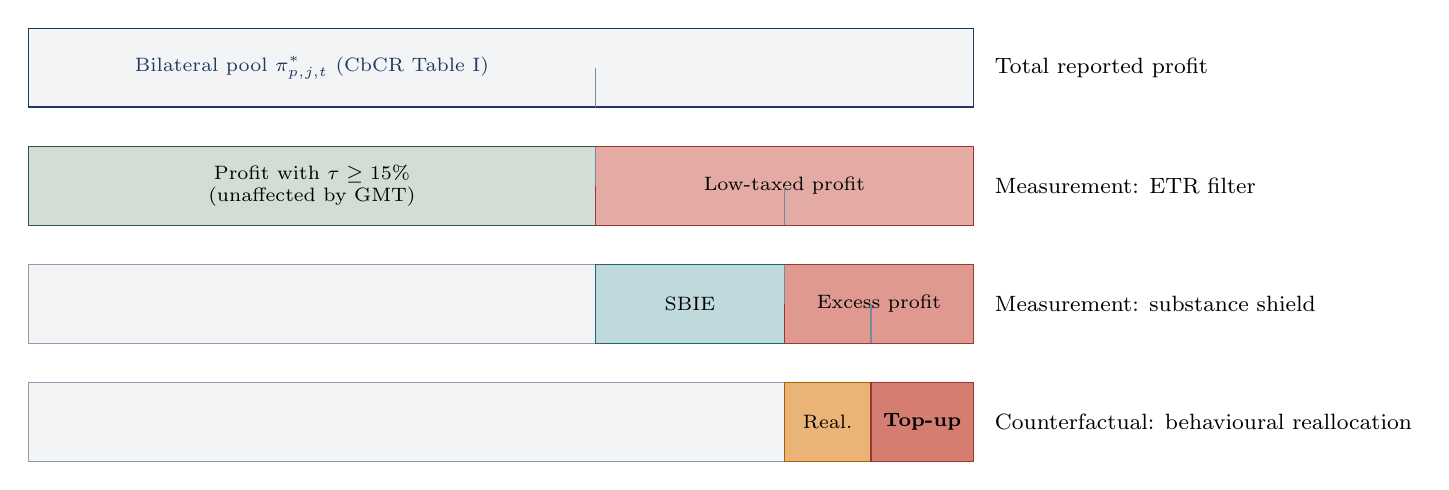
\begin{tikzpicture}[font=\small]
  % Total profit bar
  \def\tw{12}
  \def\th{1.0}

  % Layer 1: total profit
  \fill[thesisLight, draw=thesisNavy, line width=0.6pt] (0,4) rectangle (\tw, 4+\th);
  \node[font=\footnotesize, anchor=west] at (\tw+0.15, 4+\th/2) {Total reported profit};

  % Layer 2: split into above-15 (left) and below-15 (right)
  \fill[thesisGreen!25, draw=thesisGreen!70!black] (0,2.5) rectangle (7.2, 2.5+\th);
  \fill[thesisRed!45, draw=thesisRed!80!black] (7.2,2.5) rectangle (\tw, 2.5+\th);
  \node[font=\scriptsize, align=center] at (3.6, 2.5+\th/2) {Profit with $\tau \geq 15\%$\\(unaffected by GMT)};
  \node[font=\scriptsize, align=center] at (9.6, 2.5+\th/2) {Low-taxed profit};
  \node[font=\footnotesize, anchor=west] at (\tw+0.15, 2.5+\th/2) {Measurement: ETR filter};

  % Layer 3: SBIE shield on the low-taxed portion
  \fill[thesisLight, draw=thesisNavy!50] (0,1.0) rectangle (7.2, 1.0+\th);
  \fill[thesisTeal!30, draw=thesisTeal!80!black] (7.2,1.0) rectangle (9.6, 1.0+\th);
  \fill[thesisRed!55, draw=thesisRed!80!black] (9.6,1.0) rectangle (\tw, 1.0+\th);
  \node[font=\scriptsize] at (8.4, 1.0+\th/2) {SBIE};
  \node[font=\scriptsize, align=center] at (10.8, 1.0+\th/2) {Excess profit};
  \node[font=\footnotesize, anchor=west] at (\tw+0.15, 1.0+\th/2) {Measurement: substance shield};

  % Layer 4: behavioural response carves into the excess profit
  \fill[thesisLight, draw=thesisNavy!50] (0,-0.5) rectangle (9.6, -0.5+\th);
  \fill[thesisOrange!55, draw=thesisOrange!80!black] (9.6,-0.5) rectangle (10.7, -0.5+\th);
  \fill[thesisRed!70, draw=thesisRed!80!black] (10.7,-0.5) rectangle (\tw, -0.5+\th);
  \node[font=\scriptsize, align=center] at (10.15, -0.5+\th/2) {\rotatebox{0}{Real.}};
  \node[font=\scriptsize, align=center] at (11.35, -0.5+\th/2) {\textbf{Top-up}};
  \node[font=\footnotesize, anchor=west] at (\tw+0.15, -0.5+\th/2) {Counterfactual: behavioural reallocation};

  % Connecting brackets
  \draw[thesisNavy!60, line width=0.4pt] (7.2, 4) -- (7.2, 3.5+\th);
  \draw[thesisNavy!60, line width=0.4pt] (7.2, 2.5+\th) -- (7.2, 2.0+\th);
  \draw[thesisNavy!60, line width=0.4pt] (9.6, 2.5) -- (9.6, 2.0+\th);
  \draw[thesisNavy!60, line width=0.4pt] (9.6, 1.0+\th) -- (9.6, 0.5+\th);
  \draw[thesisNavy!60, line width=0.4pt] (10.7, 1.0) -- (10.7, 0.5+\th);

  % Annotations
  \node[font=\scriptsize, thesisNavy] at (3.6, 4+\th/2) {Bilateral pool $\pi^{*}_{p,j,t}$ (CbCR Table I)};
\end{tikzpicture}
}
\caption[GMT design features as successive filters.]{Three design features of the GMT, applied as successive filters to the bilateral profit pool. The ETR filter isolates the low-taxed mass (red), which the jurisdiction-average and within-jurisdiction-distributional approaches measure differently. The substance filter applies the substance-based income exclusion, shielding a fraction $\bar{\phi}_{p,j,t}$ of the low-taxed profit on the basis of payroll and tangible assets. The behavioural counterfactual removes the share that MNEs reallocate once the effective floor rises. Only the residual (dark red) yields a top-up tax. Each filter maps to one or more factors in the variance decomposition of Section \ref{sec:decomposition}.}
\label{fig:gmt_mechanics_intro}
\end{figure}

The results qualify the strongest ex-ante behavioural expectation. The 2017--2022 panel yields a statistically significant linear semi-elasticity of 1.51, with a two-way clustered $p$-value of $1.6 \times 10^{-6}$. This estimate exceeds the \citet{heckemeyer2017} consensus of 0.8, but it is far below the very steep low-rate response in \citet{dowd2017}. The Bayesian information criterion (BIC) selects the linear specification over the logarithmic alternative ($\Delta$BIC = 5.26) and the quadratic alternative ($\Delta$BIC = 7.56). The behavioural counterfactual is therefore economically relevant, reducing cumulative EU revenue by US\$47.1 billion on average across scenarios, but it does not dominate the decomposition.

The revenue results show a wider scenario range than a single headline estimate can communicate. Across the 32 scenarios, cumulative EU revenue over 2017--2022 ranges from US\$125.8 billion to US\$553.9 billion. Moving from jurisdiction-average to distributional ETR measurement raises average cumulative EU revenue from US\$195.1 billion to US\$400.7 billion. Moving from universal IIR and UTPR collection to the SbS regime reduces average cumulative EU revenue from US\$356.5 billion to US\$239.2 billion. In the preferred mechanical core scenario, the SbS regime reduces cumulative EU revenue from US\$531.6 billion to US\$362.1 billion. When the behavioural response is also applied, the corresponding figures are US\$453.0 billion and US\$309.6 billion. The SBTI analysis adds a sectoral result: the EU27 profit-weighted effective floor falls from 14.2\% before SBTI to 11.9\% after SBTI, with the largest reductions in more capital-intensive sector-country cells.


\subsection{Societal relevance}\label{sec:relevance}

The GMT already enters European public budgets, so the sensitivity of revenue estimates has practical fiscal value. The Dutch Ministry of Finance projected \EUR466 million in annual GMT revenue, with \EUR402 million, or 86\%, attributed to the behavioural response from reduced profit shifting \citep{36369_3}. The January 2026 SbS package then reduced the Dutch projection by \EUR122 million per year \citep{1028}. These revisions illustrate the policy problem studied here: a revenue forecast can move because the estimated behavioural response changes, because the measured low-taxed base changes, or because the legal allocation channel changes. The decomposition in this thesis tells these channels apart.

The distributional stakes extend beyond one national budget. Tax competition has compressed corporate tax bases across Europe \citep{cassee2019}, and low-income countries lose a disproportionate share of revenue to profit shifting \citep{cobham2018,garcia-bernardo2024}. Country-level estimates that trace projected revenue to a specific modelling choice are an input to implementation negotiations. The thesis provides those estimates for all 27 EU Member States, allowing finance ministries, the European Commission and the OECD to identify which assumption drives which number.

\subsection{Scientific contribution}\label{sec:contribution}

The thesis delivers four contributions to the GMT revenue literature. First, it provides a panel estimate of profit-shifting semi-elasticities on the post-transition OECD CbCR panel for 2017--2022 with bilateral parent--affiliate fixed effects. Earlier estimates rely on a single country \citep{dowd2017,boukal2026} or a single cross-section \citep{garcia-bernardo2024}. The panel structure absorbs time-invariant bilateral confounders, including treaty networks, legal-system similarity and persistent MNE group structure. Three functional forms are estimated on the same sample and ranked by BIC, producing directly comparable semi-elasticity schedules across the ETR distribution.

Second, the thesis embeds the estimated semi-elasticity in a $2^5$ full factorial design together with four further binary modelling choices. The 32 revenue scenarios are decomposed through an orthogonal structural variance identity that attributes variation exactly to five main effects and all their interactions. The economic interpretation follows the logic of decomposition methods: ETR measurement and substance factors change the measured endowment, while the behavioural factor changes the coefficient applied to that base \citep{oaxaca1973,blinder1973,shorrocks2013}. Existing studies vary assumptions one at a time \citep{barake2022,hugger2026} or decompose revenue by collection channel for a single country \citep{boukal2026}. The factorial design shows that interactions are present but modest in the current results, with 5.3\% of pooled variance.

Third, the thesis constructs sector-specific effective tax floors for 27 EU Member States by combining CbCR aggregate levels with EU host-country sectoral shares from post-2021 Eurostat Foreign Affiliates Statistics (FATS) and capital-stock information from EUKLEMS \& INTANProd. The datasets are complementary: CbCR has tax data but no sectoral breakdown, FATS has EU-wide foreign-control sector detail but no tax data, and EUKLEMS supplies capital-stock measures that are closer to the stock concept required by the SBIE than investment flows. The SBTI result is therefore a measured sectoral exposure estimate, not a claim that public data observe actual qualifying tax incentive claims.

Fourth, the thesis cross-validates the percentile-based distributional ETR fit from CbCR Table I against the direct subsidiary-level ETR brackets in CbCR Table IV\@. Table IV observes the profit mass below 15\% without distributional extrapolation. The validation shows where the early-year bracket-share panel imputation is stable and where it is fragile, which matters because the public CbCR panel contains detailed subsidiary-level ETR brackets only from 2019 onwards.

The remainder of the thesis is organised as follows. Section \ref{sec:litreview} reviews the profit-shifting literature, the GMT base mechanics, and theoretical models of tax competition under minimum taxation, and develops the five hypotheses. Section \ref{sec:data} introduces the data and measurement framework, showing how raw CbCR variables are transformed into the measured low-taxed profit base. Section \ref{sec:methodology} presents the econometric design, the counterfactual revenue model, and the factorial decomposition. Section \ref{sec:results} reports the empirical results. Section \ref{sec:discussion} concludes with the discussion, policy implications, and limitations.

\newpage
\section{Literature review}\label{sec:literature}\label{sec:litreview}

The literature on the GMT sits at the intersection of three older debates: how large profit shifting is, how changes in corporate income tax (CIT) interact with real economic activity, and how countries compete over corporate tax bases when there is a minimum taxation. This section walks through each debate and then pulls the three strands together into the framework that the methodology estimates. Section \ref{sec:beps} covers the empirical measurement of profit shifting, establishing the magnitudes that the GMT targets. Section \ref{sec:design} examines the GMT's design, revenue mechanics and the role of the substance-based income exclusion. Section \ref{sec:theory_lit} reviews theoretical models of tax competition under minimum taxation. Section \ref{sec:theoretical_framework} synthesises these strands into the causal chain that the methodology estimates. Throughout, the review identifies what each contribution delivers and where its limitations create the gaps that this thesis addresses.

\subsection{The empirical measurement of base erosion and profit shifting}\label{sec:beps}

The Global Minimum Tax was designed around the premise that MNEs shift substantial volumes of profit to low-tax jurisdictions, eroding the tax base of countries where real economic activity occurs. Quantifying the magnitude of this shifting has been a central concern of the literature for over three decades.

\subsubsection{Methodological foundations}

The foundational approach to estimating profit shifting is surveyed by \citet{heckemeyer2017}, who identify a consensus tax semi-elasticity of reported profits of approximately 0.8. This estimate, derived from a meta-regression of 27 studies, implies that a one percentage point reduction in the tax rate differential is associated with a 0.8\% increase in reported pre-tax profits. They also conclude that transfer pricing and strategic location of intellectual property account for approximately 82\% of observed BEPS, with debt shifting responsible for the remaining 18\%.\footnote{The 82\%/18\% split is the preferred estimate from \citet{heckemeyer2017}. An alternative calculation using the debt-ratio control yields 67\%/33\%. The range across all six specifications in their Table 5 places the non-financial share at a minimum of two thirds.} The meta-regression imposes a constant semi-elasticity across the tax rate distribution, which masks the nonlinearity that subsequent work reveals at low ETRs. \citet{dharmapala2014} surveys the empirical literature on BEPS and reaches the same consensus semi-elasticity of approximately 0.8, drawing on the \emph{Hines-Rice approach} that regresses the logarithm of reported profits on the tax rate, controlling for real economic activity through labour and capital inputs. \citet{huizinga2008} extend this framework to a multilateral setting using Amadeus data, estimating a semi-elasticity of 1.3. \citet{riedel2018} provides a subsequent review that largely confirms this consensus, noting that channel-specific studies (examining debt shifting and transfer pricing separately) tend to produce the most credible estimates.

\subsubsection{Nonlinear profit shifting}

An insight for the GMT is that profit-shifting behaviour is highly nonlinear across the tax rate distribution. \citet{dowd2017} demonstrate this using US Internal Revenue Service administrative tax return data on Controlled Foreign Corporations covering 2002--2012. Their quadratic specification reveals that the semi-elasticity at a 5\% statutory tax rate is approximately 4.7, compared to only 0.7 at a 30\% rate.\footnote{These semi-elasticities are evaluated at statutory rates, not effective tax rates. Using average (effective) tax rates, \citet{dowd2017} report a semi-elasticity of 3.1 at 5\% and $-0.5$ at 30\%. The distinction matters when applying these coefficients to CbCR effective tax rates, which average 6.9 percentage points below statutory rates \citep{hugger2026}.} This implies that a one percentage point reduction in the tax rate at the very bottom of the distribution induces nearly seven times more profit shifting than the same reduction at moderate rates. The practical consequence is sizeable: in a simulation that raises six haven jurisdictions (Bermuda, the Cayman Islands, Ireland, Luxembourg, the Netherlands and Switzerland) to a 29\% statutory rate, the quadratic model predicts a \$116 billion reduction in shifted profits, roughly double the \$55--76 billion predicted by the linear model. \citet{garcia-bernardo2024} formalise this insight by developing a \emph{logarithmic} specification for the relationship between reported profits and effective tax rates. Their methodology, applied to OECD CbCR data for 2017, yields an estimate of \$850 billion in shifted profits, higher than the \$616 billion estimated by \citet{torslov2023} for 2015, partly because the log specification better captures the concentration of shifting at very low rates. Furthermore, \citet{garcia-bernardo2024} find that lower-income countries lose a larger share of total tax revenue to profit shifting than high-income countries, a finding with direct implications for the distributional assessment of the GMT.

\subsubsection{Aggregate estimates of profit shifting}

The aggregate scale of profit shifting has been estimated through two broad approaches: micro-level firm data and macro-level national accounts. The most influential macro-level study is by \citet{torslov2023}, who use Foreign Affiliates Statistics to compare the profitability of foreign-owned and locally-owned firms within each jurisdiction. Their preferred estimate is that 36\% of multinational profits (approximately \$616 billion in 2015) were shifted to tax havens, with US multinationals shifting roughly twice as much as multinationals from other parent countries relative to the size of their foreign earnings. The European Union is the biggest loser of tax revenue, with corporate tax revenue reduced by an estimated 20\% for non-haven EU countries. Tax haven affiliates display profit-to-wage ratios that are an order of magnitude higher than those of local firms in the same jurisdiction. Their methodology relies on the assumption that locally-owned and foreign-owned firms in the same jurisdiction would earn the same return on labour absent profit shifting, an assumption that breaks down in jurisdictions where foreign firms are systematically selected into higher-productivity sectors.

\citet{garcia-bernardo2024} produce a complementary estimate using OECD CbCR data, finding that MNEs shifted over \$850 billion in 2017. Their logarithmic specification captures the extreme concentration of shifted profits at very low ETRs and identifies the Cayman Islands, Luxembourg, Singapore, the Netherlands, Switzerland, Hong Kong, Bermuda, Puerto Rico and Ireland as the primary destinations. The cross-sectional design cannot control for time-invariant bilateral confounders, and the 2017 CbCR vintage is affected by the double-counting issues that \citet{blouin2023} document. \citet{garcia-bernardo2022a} test whether the 2017 US Tax Cuts and Jobs Act (TCJA) reduced profit shifting by US MNEs. They find that the share of foreign profits booked in tax havens remained stable at approximately 50\% between 2015 and 2020, despite a 3--5 percentage-point decline in the share of profits booked abroad overall. The persistence of tax-haven profit shares after a major reform that narrowed the US--haven tax differential is indirect evidence that profit shifting responds nonlinearly to tax rate changes: the TCJA narrowed the differential at moderate rates but left the incentive at very low ETRs largely intact.

\subsubsection{The double-counting critique}

A challenge to these estimates comes from \citet{blouin2023}, who demonstrate that standard data sources (US Bureau of Economic Analysis data, US IRS Form 5471, and Orbis/Bureau Van Dijk) suffer from systematic double counting and misattribution of foreign affiliate income. The equity method of accounting causes the same dollar of profit to be counted multiple times when ownership is structured through intermediate holding companies, a practice that expanded dramatically after the 1997 US ``check-the-box'' regulations. When \citet{blouin2023} replicate the revenue loss estimate of \citet{clausing2016} using the corrected measure ``Net Income Excluding Equity Income'', the estimate falls from \$77--111 billion to approximately \$11 billion, a reduction of roughly 90\%. Their reanalysis of \citet{torslov2023} suggests that the bilateral imputation of \$306 billion in shifted profits contains substantial equity income, and that removing this component reduces the total estimate by approximately half.


\subsubsection{Firm-level evidence}

\citet{johansson2017} provide large-scale firm-level evidence using the Orbis database, with 1.2 million observations across multiple countries. They find that the largest MNEs reduce their effective tax rates by 4--8.5 percentage points through a combination of profit shifting and the exploitation of tax mismatches. The estimated global corporate income tax revenue loss ranges from 4\% to 10\%. \citet{bilicka2026} exploit variation in German municipal business tax rates across over 11{,}000 municipalities during 2008--2019, finding that subsidiaries of MNEs with affiliates in tax havens respond significantly more to local tax rate increases than other firms. After a rate increase, tax revenues decline in municipalities more exposed to these aggressive MNEs, while real activities (assets and employment) remain unchanged, consistent with profit reallocation rather than real relocation. The finding supports the nonlinear profit-shifting response: firms with existing low-tax structures shift more aggressively at the margin.

The representativeness of firm-level databases is itself a methodological concern. \citet{kalemli-ozcan2015} provide critical guidance on constructing nationally representative samples from Orbis. \citet{torslov2023} show that Orbis lacks data in low-tax jurisdictions where publishing financial statements is not mandatory. For the US, Ireland, and Switzerland, no income data are available. In 2012, only 17\% of global profits appeared in Orbis, and over 80\% of subsidiaries were unknown to the database.

\subsubsection{Effects of transparency on profit shifting}

\citet{tuinsma2025} exploit the EUR 750 million revenue threshold for CbCR filing in a regression discontinuity design using Orbis data on EU-headquartered MNEs. Private CbCR raised ETRs of affected MNEs by approximately 6 percentage points relative to firms just below the threshold. The effect is concentrated in moderately aggressive firms (low pre-CbCR ETRs but no tax-haven affiliates); the most aggressive MNEs with established haven structures showed only moderate responses. The finding implies that the CbCR panel used in this thesis captures a population whose tax behaviour was itself shifting during the sample period, a consideration for the panel estimation (Section \ref{sec:estimation}).

\subsection{GMT design, revenue mechanics and implementation}\label{sec:design}

\subsubsection{Revenue estimates}

\citet{barake2022} provide the first systematic estimate of GMT revenue effects under Pillar Two. Using a combination of CbCR and FATS data, they calculate that a 15\% minimum effective tax rate would generate approximately \EUR 179 billion globally\footnote{This figure assumes that all profit within a jurisdiction faces the jurisdiction-average ETR, either fully above or fully below 15\%. As \citet{hugger2026} demonstrate, 53.2\% of globally low-taxed profit lies in jurisdictions with above-15\% average ETRs, so the true GMT base is substantially larger than Barake's estimate implies. \citet{barake2022} acknowledge this limitation but lack the within-jurisdiction ETR data needed to correct it.} and \EUR 55 billion within the EU, under an IIR-first scenario. These are first-stage estimates that assume no behavioural response by MNEs. The actual revenue depends critically on whether the top-up tax is collected by the jurisdiction of the ultimate parent entity through the IIR, or by the source country through a QDMTT.

\citet{janeba2023} develop a strategic tax competition model that produces a more nuanced picture. Their finding is that the revenue effect of the GMT depends on whether governments use distortionary or lump-sum instruments to compete for real economic activity. When instruments are distortionary, the GMT reduces profit shifting but may intensify competition among non-haven countries for real investment, potentially offsetting a portion of the revenue gains.

\subsubsection{The substance-based income exclusion}

A feature of the GMT is the SBIE, which excludes from the top-up tax calculation an amount equal to a percentage of eligible payroll costs and tangible assets located in each jurisdiction. During the transition period (2024--2033), the carve-out starts at 10\% of payroll and 8\% of tangible assets, declining to 5\% of each. \citet{devereux2023} provide the first empirical assessment of the SBIE using Amadeus data on foreign-owned EU subsidiaries, finding that the average ratio of SBIE to pre-tax profit is 57\% (52\% median), declining to 41\% (28\% median) after the ten-year transition. This implies that the average minimum tax on GloBE income is only 6.45\% in the first transition year, rising to 8.85\% at long-run rates, well below the headline 15\%. Approximately 30\% of foreign-owned EU subsidiaries in scope have SBIE exceeding pre-tax profit, facing zero top-up tax regardless of their ETR.

\citet{schjelderup2024} analyse the economic implications of the SBIE within a formal model. They reach the conclusion that the SBIE functions as a \emph{de facto} production subsidy in low-tax jurisdictions. By tying the exclusion to tangible assets and payroll, the GMT inadvertently incentivises MNEs to increase their real economic presence in low-tax locations, thereby expanding the exclusion and reducing the top-up tax. This creates a capital demand distortion that partially offsets the reduction in transfer pricing distortions that the GMT otherwise achieves. Quantitatively, the effective reduction in the rental cost of capital (0.50--0.96\%) exceeds the reduction in the effective wage rate (up to 0.88\%), implying that the SBIE \emph{favours capital-intensive industries}.

\subsubsection{Within-jurisdiction heterogeneity}

\citet{hugger2026} provide what is the most important empirical finding for understanding the actual reach of the GMT. Using confidential ETR data at the MNE-jurisdiction level, they demonstrate that 53.2\% of all low-taxed profit (below 15\% ETR) is located in jurisdictions where the \textit{average} ETR exceeds 15\%. The within-jurisdiction dispersion in ETRs is often larger than the cross-jurisdiction dispersion. This finding implies that jurisdiction-level analyses (which use average ETRs) substantially underestimate the amount of low-taxed profit and, correspondingly, the potential revenue from the GMT.

\subsubsection{Tax incentives under Pillar Two}

\citet{ferreiraliotti2022} examine how existing tax incentives interact with the GMT. The impact varies dramatically by type: accelerated depreciation provisions have a low impact because they primarily affect timing rather than the level of taxation, whereas tax holidays and IP box regimes have a significant impact because they reduce the ETR below 15\%. The QDMTT serves as a safety valve that allows countries to retain the top-up tax domestically, but this also means that the incentive offered to the MNE is effectively nullified.

\subsection{Theoretical models of the GMT and tax competition}\label{sec:theory_lit}

\subsubsection{Welfare effects}

\citet{johannesen2022} develops the first formal model specifically designed to analyse the welfare effects of the GMT. The model features a large country (non-haven) and a small country (haven) that compete for mobile profits. The central result is that the welfare effect for the non-haven country is \textit{ambiguous}: it is positive when the profit-shifting response to taxation is strong and when the government places a low weight on the consumption of firm owners relative to public goods. The consensus semi-elasticity of 0.8 falls below even the lowest of the required thresholds (which range from roughly 1.8 to 4.2 depending on the marginal social value of public funds and the initial haven tax rate; Table 1 in \citealp{johannesen2022}), but the quadratic specification of \citet{dowd2017} exceeds them all at ETRs below roughly 9\%, precisely the range in which the GMT base is concentrated.

\citet{hebous2023} contribute to this debate by identifying conditions under which a minimum corporate tax can be Pareto-improving: all countries, including havens, can be made better off if the minimum tax is combined with appropriate transfers. \citet{vantriet2025} provide the first quantitative welfare assessment, simulating the GMT in the CORTAX macroeconomic model for the EU-27, the US, the UK, Japan, and a generic tax haven. Under their preferred closure (additional CIT revenue recycled as lower CIT rates), the GMT produces modestly positive global welfare, and the optimal minimum rate is 16\%. The simulation satisfies the Hicks--Kaldor compensation test, indicating a potential Pareto improvement. Their model does not incorporate the nonlinear semi-elasticities that \citet{dowd2017} document, however, and uses a representative-firm framework that cannot capture within-jurisdiction ETR heterogeneity.

\subsubsection{Tax competition under the GMT}

\citet{janeba2023} model the strategic interaction between countries after GMT implementation. Their model distinguishes between profit-shifting channels (which the GMT constrains) and real-activity channels (which it does not). The GMT eliminates the incentive for havens to set rates below 15\%, but it simultaneously increases the incentive for non-havens to compete for real economic activity through subsidies, infrastructure investment, and regulatory competition.

\citet{schjelderup2024} extend this analysis by incorporating the SBIE into a two-country model. They show that the SBIE transforms the GMT from a pure anti-avoidance instrument into a hybrid policy that simultaneously discourages profit shifting (through the minimum tax) and encourages real investment in low-tax jurisdictions (through the substance exclusion). The net effect on the allocation of capital is theoretically ambiguous and depends on the elasticity of transfer pricing relative to the elasticity of real capital demand.

\subsubsection{The enforcement dilemma}

\citet{jean2026} introduce a fundamentally different concern: the GMT may undermine the international cooperation that is necessary for effective tax enforcement. In their game-theory model, two countries (high-tax and low-tax) choose both tax rates and enforcement effort. The GMT reduces the incentive for the low-tax country to cooperate on enforcement, because the top-up tax is collected by the high-tax country. When the minimum rate exceeds a critical threshold, the low-tax country prefers to withdraw from enforcement cooperation entirely. This creates a paradox: the GMT reduces profit shifting in the short run but may increase it in the long run by destroying the cooperative enforcement equilibrium.

\subsection{Theoretical framework}\label{sec:theoretical_framework}

The three strands above converge on a mechanism. A minimum tax at rate $T$ raises the marginal rate on every euro of low-taxed profit from the pre-reform ETR $\tau_{j,t}$ to $T$, and reported profits in each affected jurisdiction contract in proportion to the curvature of the concealment cost. Revenue at the source is therefore the product of three filters: the profit mass below the floor, the share of that mass not shielded by the SBIE, and the share that survives behavioural relocation. This decomposition is the reduced form of the optimality condition in \citet{johannesen2022}: Lemma 2 establishes the $t_L \mapsto \max(t_L, T)$ substitution, and the Hines--Rice regression of \citet{hines1994} identifies the derivative of optimal shifted profit with respect to the applicable rate. Each filter maps to an estimable object, and the shape of the semi-elasticity governs two of them.

The literature has not settled that shape. \citet{heckemeyer2017} impose constancy at 0.8, \citet{dowd2017} fit a quadratic that rises to 4.7 at a 5\% rate, and \citet{garcia-bernardo2024} fit a logarithm that diverges as the rate approaches zero. The GMT base is concentrated precisely where the specifications disagree most, so committing to any single form before estimation is a prejudgement of the revenue answer. Estimating all three on the same sample and ranking them replaces that prejudgement with a model-selection decision. The 2017--2022 OECD CbCR panel makes the decision tractable: pair fixed effects absorb time-invariant bilateral confounders (treaty networks, legal-system similarity, persistent MNE group structure), and within-pair variation from domestic CIT reforms, the 2017 TCJA, and the pandemic-era profit compression identifies the tax coefficient. \citet{dowd2017} estimate on a US-only CFC panel with no cross-country variation; \citet{garcia-bernardo2024} estimate on a single 2017 CbCR cross-section. The combined cross-country, multi-year design here is original to this thesis.

Three further modelling choices sit on top of the semi-elasticity question, each pulling revenue in a different direction. The within-jurisdiction dispersion documented by \citet{hugger2026} means that jurisdiction-average and distributional ETR measures recover different low-taxed masses. The SBIE can be measured with the aggregate public-CbCR carve-out proxy or with an EU host-country sectoral bridge that imposes FATS sector shares and EUKLEMS capital-stock shares on the aggregate CbCR base. The latter is a sensitivity, not the preferred point estimate. The transitional and long-run carve-out rates bracket a plausible range. The January 2026 Side-by-Side Safe Harbour carves US-parented groups out of the IIR and UTPR channels while leaving QDMTTs operational. The pipeline is multiplicative, which guarantees that these choices interact: the behavioural response compounds the distributional base, the SBIE specification modulates the shield that sits between them, and the SbS carve-out redirects the surviving liability. One-at-a-time sensitivity, the standard in \citet{barake2022} and \citet{hugger2026}, cannot expose these interactions. A $2^5$ full factorial design over the five binary choices, decomposed through orthogonal structural variance contrasts, makes them visible and exactly attributable. The factorial framing is new to the GMT revenue literature.

\newpage

\section{Data}\label{data}\label{sec:data}\label{sec:descriptive}

This section first describes the collection of the data. The panel consitsts of a cleaned parent--affiliate--year dataset that turns public Country-by-Country Reporting (CbCR) aggregates into corrected profit, effective tax rate (ETR) support, low-taxed profit, substance-based carve-out inputs and legal allocation flags. The empirical analysis builds mainly on Country-by-Country Reporting (CbCR) data, because these data connect multinational profit, tax, turnover, employees, tangible assets and related-party activity to the jurisdictions where firms report them. The data do not observe every firm-level decision. They do, however, provide the closest available aggregate view of where multinational groups report income and economic substance.

\subsection{OECD CbCR data}\label{CbCR}

BEPS Action 13 requires large MNE groups with consolidated revenue exceeding \EUR750 million to file Country-by-Country Reports detailing their economic activity and tax payments in each jurisdiction where they operate.\footnote{The \EUR750 million threshold was chosen by the OECD to balance coverage against compliance burden. Since Pillar Two applies to the same threshold population, the CbCR scope aligns with the GMT's statutory scope. The threshold excludes smaller MNEs that may face systematically different ETRs. This is not a limitation for revenue estimation but matters for welfare analysis.} The OECD aggregates and anonymises these filings into jurisdiction-level statistics published in the Corporate Tax Statistics (CTS) database.\footnote{The data can be found via the OECD Data Explorer, Taxation, Corporate Tax. Under this view, as of April 2026, 19 datasets appear. The six CbCR tables can be filtered out of these. This \href{https://data-explorer.oecd.org/?fs\%5B0\%5D=Topic\%2C1\%7CTaxation\%23TAX\%23\%7CCorporate\%20tax\%23TAX_CPT\%23&pg=0&fc=Topic&bp=true&snb=19}{link} also references the data.}

The CbCR dataset is suited for GMT revenue estimation, since it captures tax-planning behaviour across virtually all jurisdictions, including low-tax locations that are absent from firm-level databases such as Orbis or Compustat.\footnote{Firm-level databases suffer from selection bias in low-tax jurisdictions because MNEs operating through shell entities in these locations often have no obligation to file public financial statements \citep{torslov2023}. CbCR data are filed with the parent jurisdiction's tax authority and reported to the OECD regardless of the affiliate jurisdiction's disclosure regime \citep{oecd2025a}.} Second, the bilateral parent--affiliate structure mirrors the GMT's own architecture: the top-up tax is computed jurisdiction by jurisdiction for each MNE group, allocated through the Income Inclusion Rule to the parent and, where no parent IIR applies, through the UTPR to implementing jurisdictions with observed group activity. 

The most recent public CbCR release covers fiscal year 2022, published in November 2025 \citep{oecd2025a}. The lag of approximately three years between fiscal year and public availability means that post-implementation CbCR outcomes are not yet observed. The estimation is therefore necessarily backward-looking: it applies the GMT rules to pre-implementation data and projects revenue prospectively. The main empirical sample starts in 2017. The OECD treats 2016 as a transition vintage because filing was still voluntary in part of the sample and the fiscal-year window differs from later releases, and \citet{hugger2026} likewise exclude 2016 from their baseline ETR construction. The resulting 2017--2022 panel still provides six pre-reform years of within-pair variation, which is sufficient for the identification strategy developed in Section \ref{sec:estimation}.

The CbCR database is organised into six tables, each constructed from the same underlying filings but aggregated along different dimensions. Table \ref{tab:crosssummary} summarises their structure. Coverage expanded substantially over the period as more jurisdictions enacted BEPS Action 13 legislation: 26 parent jurisdictions reported in 2016, rising to 54 by 2022, representing approximately 98\% of all CbCR filings globally \citep{oecd2025a}.

\begin{table}[H]
\centering
\caption{Cross-table summary of OECD CbCR Tables I--VI}
\label{tab:crosssummary}
\footnotesize
\begin{tabular}{@{}lrrrrrrr@{}}
\toprule
 & \textbf{Table I} & \textbf{Table II} & \textbf{Table III} & \textbf{Table IV} & \textbf{Table V} & \textbf{Table VI} \\
 & Agg.\ Totals & IQ Means & ETR (MNE) & ETR (Sub.) & Size Dist.\ & Size Agg.\ \\
\midrule
Rows (total) & 1,124,211 & 437,129 & 699,246 & 101,399 & 4,195 & 105,753 \\
Positive obs (\%) & 71.5 & 84.6 & 68.3 & 77.3 & 98.4 & 72.1 \\
Zero obs (\%) & 21.7 & 7.6 & 24.9 & 12.1 & 0.4 & 22.9 \\
NaN / missing (\%) & 3.0 & 1.9 & 3.6 & 6.5 & 1.1 & 2.4 \\
\addlinespace
Fiscal years covered & 2016--2022 & 2017--2022 & 2017--2022 & 2016--2022 & 2016--2022 & 2022 only \\
Parent jurisdictions & 58 & 46 & 46 & 49 & 40 & 39 \\
Affiliate jurisdictions & 240 & 238 & 238 & 154 & -- & 215 \\
Number of MEASURE codes & 28 & 14 & 27 & 27 & 3 & 26 \\
\addlinespace
Aggregation type & \code{TOTAL} & \code{TOTAL} & \code{TRMNE} & \code{TRSUB} & \code{TRMNE} & \code{MNESIZE} \\
ETR brackets & No & No & Yes (12) & Yes (11) & No & No \\
Profit panels & A-I, A-II & A-I, A-II & -- & -- & -- & -- \\
Statistical operations & Pct., Agg & IQmean & Agg & Agg & Pctiles & Agg \\
MNE size classes & No & No & No & No & No & Yes (6) \\
\bottomrule
\end{tabular}
\end{table}

Tables I and IV are mostly used in this paper. They complement each other: Table I supplies the aggregate financial levels together with summary percentiles of the within-jurisdiction ETR distribution, while Table IV partitions the same financial variables into 11 ETR brackets at the subsidiary level. Neither table dominates the other. Table I has broader coverage (58 vs.\ 49 parents and 240 vs.\ 154 affiliate jurisdictions) and is the only source of percentile moments ($P5, P25, P50, P75, P95$); Table IV has narrower coverage but observes directly the profit mass inside the GMT-critical $[0, 15\%)$ bracket. The measurement framework therefore uses Table I for distributional fitting and Table IV for direct observation, combining them in the hybrid measurement of Section \ref{sec:crossval}. The other four tables supply supporting information (Section \ref{sec:other_tables}).

Public CbCR profit data suffer from systematic double counting through intra-group dividends and ownership chains. When a German parent owns a Dutch holding company that in turn owns an Irish operating subsidiary, the Irish subsidiary's profits may appear in both the German CbCR filing, through the ultimate parent, and in the Dutch profits, through the intermediate holding company. \citet{blouin2023} identify the accounting mechanism: equity income is booked where ownership claims sit, so the same operating profit can appear again in a domestic UPE or holding-company location. \citet{garcia-bernardo2022a} show the aggregate importance for public CbCR data: reported profits are overstated by 48\% in 2017, 72\% in 2018 and 47\% in 2019, with domestic American profits responsible for much of the discrepancy. The correction therefore cannot be a uniform haircut on every foreign affiliate cell. It must be targeted to the cells where equity income can plausibly be reported.

\input{generated/results_tables/profit_correction_effects.tex}

Table \ref{tab:profit_correction_effects} reports the implemented profit-base correction. The correction reduces positive-profit CbCR profit by US\$12.0 trillion over 2017 to 2022, a reduction rate of 25.6\%. Almost all of that adjustment comes from domestic ultimate-parent locations, where double counting through equity income is most plausible. The observed \code{PROFIT\_ADJ} sample contains only 36 cells and is therefore used as diagnostic support rather than as a donor sample for a full-panel imputation.

The cleaned panel is reported in Tables \ref{tab:data_panel_coverage} and \ref{tab:data_summary_statistics}. It shows the number of parent-affiliate-year cells that survive the cleaning rules, the scale of the corrected profit base, the measured low-taxed profit mass and the moments of the variables that enter the measurement and econometric stages.

\input{generated/data_descriptive_tables.tex}

Three features of the data are important for the rest of the thesis. First, the main 2017 to 2022 panel contains 15{,}758 analytical pair-years, of which 11{,}872 have positive corrected profit and can therefore generate top-up tax. The reporting base expands from 38 parent jurisdictions in 2017 to 54 in 2022, so year fixed effects are necessary in the behavioural model. Second, the financial variables are extremely right-skewed: the mean corrected-profit cell is US\$2.9 billion, while the median is only US\$77.1 million. This is why the Hines-Rice specification works in logs and why country-influence diagnostics are required later. Third, the median bounded ETR is close to the 15\% threshold, but the median distributional low-taxed share is 39.8\%. This confirms that the relevant empirical question is not merely whether a jurisdiction-average ETR falls below 15\%, but how much profit inside the jurisdiction lies below the threshold.

The full correction pipeline is documented in Appendix \ref{app:measurement_framework}, while Appendix Sections \ref{app:data}, \ref{app:unit_obs} and \ref{app:sector} document the data units, CbCR construction and sectoral bridge. The next subsection explains how the sectoral bridge is layered on top of the cleaned bilateral base.

\subsection{Sectoral decomposition}\label{sec:sectoral_data}

CbCR reports no sectoral breakdown. The substance-based income exclusion depends on payroll and tangible assets, both of which vary dramatically across sectors: manufacturing has high payroll and capital intensity relative to profits, while holding and IP licensing have near-zero substance. Estimating sector-specific SBIE-to-profit ratios and effective tax floors (Section \ref{sec:sbie_decomp}) therefore requires a sectoral decomposition of economic activity that CbCR cannot provide. Eurostat inward FATS supplies the EU host-country sectoral exposure map, while EUKLEMS \& INTANProd supplies a stock-based tangible-capital allocation for the asset leg.

FATS covers all foreign-controlled enterprises operating inside European reporting economies, recording employment, turnover, value added, personnel costs and investment by NACE sector and controlling country.\footnote{``Foreign-controlled'' is defined by majority ownership (more than 50\% of voting rights) by an entity resident outside the reporting country. The definition is broader than the CbCR in-scope population: FATS includes all foreign-controlled firms regardless of size, whereas CbCR is restricted to MNE groups with consolidated revenue above \EUR750 million. The implementation uses the FATS \code{WRL\_REST} controlling-country total to isolate foreign-controlled activity and excludes overlapping aggregate NACE rows before computing shares. The FATS sectoral bridge is therefore a host-country exposure scenario, not the preferred point estimate for in-scope Pillar Two groups.} This breadth is a weakness for direct GMT measurement but a strength for sectoral relevance. Eurostat reports that foreign-controlled enterprises represented only 1\% of EU market producer enterprises in 2023, but accounted for 24.0\% of EU value added and 15.5\% of employment in business market producers \citep{eurostat2025fats}. The dataset is therefore relevant for MNE activity, while still being insufficient for GloBE ETR measurement.

Sectoral tangible assets are decomposed using EUKLEMS \& INTANProd capital-stock shares. The relevant EUKLEMS variable is the tangible capital stock, with intangible capital used only as a robustness and interpretation device because the SBIE excludes most intangible assets. Where EUKLEMS is available only at a broader NACE level than FATS, the broader stock share is retained and FATS is used only to distribute activity within that sectoral family. 

The CbCR $\times$ FATS $\times$ EUKLEMS combination restricts the sectoral analysis to the EU-27.\footnote{Three grounds justify this scope. First, all 27 EU Member States appear in both CbCR Table I and Table IV as affiliate jurisdictions. Second, FATS is an EU-specific dataset with no equivalent coverage for non-EU jurisdictions. Third, the EU implemented Pillar Two uniformly through the Minimum Tax Directive (Council Directive (EU) 2022/2523), so the institutional setting is homogeneous across the sample.}

The hierarchy is set out in Appendix \ref{app:measurement_framework}.

\subsection{Supplementary data sources}\label{sec:supplementary}

The panel estimation (Section \ref{sec:estimation}) and the revenue allocation stage (Section \ref{sec:sbs}) require several additional datasets. Statutory corporate income tax rates from the OECD Tax Database (144 jurisdictions, 2000--2025) serve two purposes: as a benchmark against which CbCR effective tax rates are compared, and as an instrument in robustness checks where the endogeneity of effective rates is a concern.

The public CbCR template does not report payroll, so the payroll leg of the substance carve-out has to be reconstructed from \code{EMPLOYEES} and an external wage benchmark. Wage data are collected from three sources to maximise country coverage. OECD average annual wages (41 countries, 1990--2024) provide the primary cross-country comparator in PPP-adjusted USD. ILO hourly and monthly earnings (105--140 countries, 1990--2025) extend coverage to non-OECD economies. Wage data enter the estimation framework as the direct input to the SBIE payroll base. The base panel uses a strict source hierarchy for the affiliate-year wage $\bar{w}_{j,t}$: OECD annual average wages in PPP USD first; where missing, ILO monthly earnings in PPP USD annualised by twelve; and only as a last resort ILO monthly earnings in USD annualised. Within each source the nearest available year for the same jurisdiction is used. The constructed base is $\hat{W}_{p,j,t} = N_{p,j,t} \cdot \bar{w}_{j,t}$ (Section \ref{sec:payroll_imputation}). The same wage series also enters the Hines--Rice regression as the logarithm of the payroll proxy, controlling for affiliate-jurisdiction labour market conditions.

World Bank macroeconomic controls (GDP per capita (current USD, 217 countries, 2015--2024) and population (217 countries, 2015--2024)) enter the Hines--Rice regression as affiliate-jurisdiction controls.\footnote{Appendix \ref{app:data}, Table \ref{tab:data_sources_units}, documents the units and role of these variables.} Log GDP per capita proxies for the level of economic development and market size. Log population controls for country scale.

OECD BEPS implementation indicators document the adoption of anti-avoidance measures across jurisdictions: CbCR filing requirements (Action 13, 119 countries), CFC rules (146 countries), interest limitation rules (Action 4, 146 countries), hybrid mismatch rules (Action 2, 145 countries), IP regimes (Action 5, 64 countries), and mandatory disclosure rules (Action 12, 145 countries).\footnote{Appendix \ref{app:data}, Table \ref{tab:data_sources_units}, documents the implementation-data unit and its role in the panel.} These indicators enter the factorial design as controls for the institutional environment: jurisdictions with more comprehensive BEPS implementation may exhibit different profit-shifting patterns.

Pillar Two implementation status is tracked through the PwC global Pillar Two tracker, which records the legislative status (enacted, consultation, or announced) of the IIR, UTPR, and QDMTT for each jurisdiction, together with effective start dates.\footnote{Appendix \ref{app:data}, Table \ref{tab:data_sources_units}, documents this source, which is cross-referenced against the OECD Central Record of Qualified Domestic Minimum Taxes.} The QDMTT indicator ($\mathbb{1}_j^{\text{Q}}$) and the SbS regime indicator ($\mathbb{1}_p^{\text{SbS}}$) used in the revenue allocation stage (Section \ref{sec:sbs}) are constructed from this tracker.

\subsection{Notation}\label{sec:notation}

Subscript $p$ denotes the parent jurisdiction (ultimate parent entity, UPE), $j$ denotes the affiliate jurisdiction, and $t$ denotes the fiscal year ($t \in \{2016, \ldots, 2022\}$). The $p,j$ convention follows \citet{barake2022}; $j$ is reserved exclusively for the affiliate jurisdiction throughout. All monetary values are in USD unless stated otherwise, consistent with CbCR reporting conventions.\footnote{CbCR data are reported in USD. No PPP adjustment is applied to the revenue calculations, since the GMT operates on nominal profit and tax liabilities denominated in the MNE group's reporting currency. PPP-adjusted wage data from the OECD and ILO are used only as the input to the wage-based payroll proxy $\hat{W}_{p,j,t}$ (Section \ref{sec:payroll_imputation}).} Table \ref{tab:notation} summarises the symbols used throughout.

\begin{table}[H]
\centering
\caption{Variable notation}
\label{tab:notation}
\small
\begin{tabular}{@{}ll@{}}
\toprule
Symbol & Definition \\
\midrule
$\pi_{p,j,t}$ & Reported profit before income tax (CbCR \code{PROFIT}) \\
$\pi_{p,j,t}^{*}$ & Corrected profit base (Section \ref{sec:doublecounting}) \\
$\theta_{p,j,t}$ & Income tax accrued (CbCR \code{TAX\_ACCRUED}) \\
$A_{p,j,t}$ & Tangible assets excl.\ cash and equivalents (CbCR \code{ASSETS}) \\
$\hat{W}_{p,j,t}$ & Wage-based payroll proxy for the SBIE, constructed as $N_{p,j,t} \cdot \bar{w}_{j,t}$ (Section \ref{sec:payroll_imputation}) \\
$N_{p,j,t}$ & Number of employees, FTE (CbCR \code{EMPLOYEES}) \\
$\bar{w}_{j,t}$ & Average annual wage in jurisdiction $j$ (OECD/ILO) \\
$\tau_{p,j,t}$ & Effective tax rate (ETR) $= \theta_{p,j,t} / \pi_{p,j,t}$ \\
$T$ & Global minimum tax rate $= 0.15$ \\
$\tau_{p,j,t}^{(k)}$ & $k$-th percentile of the ETR distribution (from Table I) \\
$s_{j,t}^{<T}$ & Share of profit with ETR below $T$ in jurisdiction $j$ \\
$\ell_{p,j,t}$ & Low-taxed profit volume $= s_{j,t}^{<T} \cdot \pi_{p,j,t}^{*}$ (Section \ref{sec:etr_measurement}) \\
$\bar{\delta}_{j,t}^{\text{top}}$ & Average top-up rate on the low-taxed portion (Section \ref{sec:etr_measurement}) \\
$\tau_{j,t}^{\text{low},e}$ & Implied ETR of the low-taxed slice under ETR measurement branch $e$, $T-\bar{\delta}_{j,t}^{\text{top},e}$ \\
$\sigma_W(t), \sigma_A(t)$ & SBIE payroll and tangible assets carve-out rates (Section \ref{sec:SBIE}) \\
$\phi_{p,j,t}$ & SBIE-to-profit ratio $= \text{SBIE}_{p,j,t} / \pi_{p,j,t}^{*}$ (Section \ref{sec:SBIE}) \\
$\text{SC}_{p,j,t}^{\text{M1}}$ & Substance Cap, Method 1 (Section \ref{sec:sbti}) \\
$\text{SC}_{p,j,t}^{\text{M2}}$ & Substance Cap, Method 2 (Section \ref{sec:sbti}) \\
$\kappa_{j,s,t}$ & Sectoral SBTI-capacity proxy (Section \ref{sec:sbti_amplification}) \\
$\beta_{j,t}^{e,m}$ & Fraction of low-taxed profit reallocated under ETR branch $e$ and semi-elasticity model $m$ \\
$\mathbb{1}_j^{\text{Q}}$ & Indicator: $=1$ if jurisdiction $j$ has implemented a QDMTT \\
$\mathbb{1}_p^{\text{IIR}}$ & Indicator: $=1$ if parent jurisdiction $p$ has implemented the IIR \\
$\mathbb{1}_s^{\text{UTPR}}$ & Indicator: $=1$ if collector jurisdiction $s$ has implemented the UTPR \\
$\mathbb{1}_p^{\text{SbS}}$ & Indicator: $=1$ if parent $p$ has a Qualified SbS Regime (currently US only) \\
$\omega_{s,p,t}^{\text{U}}$ & Parent-year substance weight used to allocate UTPR pools across collector jurisdictions \\
$a_{s,p,j,t}^{(r)}$ & Allocation weight under policy regime $r$ (Section \ref{sec:sbs}) \\
$\mathbf{x}$ & Factorial configuration vector $(x_1, \ldots, x_5) \in \{0,1\}^5$ (Section \ref{sec:decomposition}) \\
$\eta_i^2$ & Share of explained variance attributable to factor $i$ (Section \ref{sec:decomposition}) \\
$\Lambda_{j,t}$ & Ratio of scenario spread to estimation uncertainty (Section \ref{sec:two_uncertainties}) \\
\bottomrule
\end{tabular}
\end{table}

\section{Measurement framework}\label{sec:measurement_framework}

After that, the section explains how the thesis turns these data into an measurement framework. It first describes the country-by-country reporting data and the adjustments needed to make them consistent across jurisdictions. It then introduces the sectoral data used to capture differences in profit rates, asset intensity and economic substance across industries. Finally, it sets out the additional data used to complete the analysis, including statutory tax rates, macroeconomic controls and jurisdiction-level classifications. 

The measured low-taxed profit base is constructed in a sequence of transparent transformations. A raw CbCR profit observation is first corrected for identifiable double counting, then matched to an ETR measurement, converted into the share and volume of profit below the 15\% threshold, reduced by the measured SBIE shield, and finally linked to legal allocation indicators. 

\subsection{Measurement of effective tax rates and low-taxed profit}\label{sec:etr_measurement}

This measurement step identifies how much profit is reported at an ETR below the 15\% threshold of the GMT and by how much that ETR falls short of 15\%. Two scalars summarise this: the share of profit with ETR below 15\% ($s_{j,t}^{<T}$) and the profit-weighted average top-up rate on that low-taxed portion ($\bar{\delta}_{j,t}^{\text{top}}$). Their product is the per-unit-profit top-up liability before the SBIE and behavioural counterfactual are applied.

Three sources of information about the within-jurisdiction ETR are available in the CbCR. Each has a different granularity and coverage trade-off. First, the \emph{profit-weighted jurisdiction-average} ETR, obtained from Table I by summing \code{TAX\_ACCRUED} and \code{PROFIT} across parent jurisdictions (Section \ref{sec:etr_calc}). Second, the \emph{distribution} of ETRs inside a jurisdiction, summarised by five bilateral percentiles ($P5, P25, P50, P75, P95$) reported only in Table I (Section \ref{sec:distributional}). Third, the \emph{direct profit mass} inside the $[0, 15\%)$ bracket, reported at subsidiary level in Table IV's \code{RATE\_0-15} cell.

These three sources capture different layers of the same measurement problem. Source (1) is used for the full 2017--2022 main sample. Source (2) is populated only from 2021 onwards (Section \ref{sec:t1_main}). Source (3) is developed bilaterally from 2019 onwards (Section \ref{sec:t4_main}). The 2019--2022 EU slice therefore admits a direct Table IV measurement, the 2021--2022 global slice admits a percentile-fit distributional measurement, and the 2017--2018 EU slice has neither. Collapsing Factor 1 to its jurisdiction-average level across the four pre-2019 fiscal years would mechanically discard precisely the within-jurisdiction heterogeneity the reform targets, so this thesis uses a hierarchical selection rule: direct Table IV where available, otherwise the Table I constrained-Beta fit, then the BSPI anchor, and finally the jurisdiction-average fallback. All four measurement branches are reconciled through a single selector that picks the most informative source actually observed for each $(j,t)$ cell.

\subsubsection{Jurisdiction-average ETR calculation}\label{sec:etr_calc}

Under the \emph{jurisdiction-average approach}, the profit-weighted average ETR across all parent jurisdictions reporting affiliates in $j$ is computed as $\bar{\tau}_{j,t} = \sum_p \theta_{p,j,t} / \sum_p \pi_{p,j,t}$. If this aggregate ratio equals or exceeds 15\%, the entire profit base of jurisdiction $j$ is treated as above the GMT threshold and no top-up tax is charged. If it falls below 15\%, the full profit base is treated as low-taxed. The approach therefore ignores within-jurisdiction heterogeneity. The basic effective tax rate for each bilateral pair $(p, j, t)$ is computed using CbCR Table I, restricting to profit-making entities:\footnote{Tax accrued (\code{TAX\_ACCRUED}) is used as the ETR numerator. Accrued taxes reflect the current-year charge, unlike taxes paid (cash basis) which include timing differences. The GloBE ETR uses ``covered taxes,'' which differ from both accrued and paid taxes and require at least 22 adjustments from the financial accounting starting point \citep{hanlon2023}. Accrued taxes are the closest available proxy in CbCR data.}
\begin{equation}\label{eq:etr}
\tau_{p,j,t} = \frac{\theta_{p,j,t}}{\pi_{p,j,t}}, \quad \text{where } \pi_{p,j,t} > 0
\end{equation}

\subsubsection{Within-jurisdiction ETR calculation}\label{sec:distributional}

The key object is the within-jurisdiction ETR distribution, because the GMT applies to the low-taxed mass inside a jurisdiction even when its average rate is above 15\%.

Averaging the ETR across all profit in a jurisdiction hides the story the reform cares about. The reform taxes each euro of low-taxed profit, not the average rate on the aggregate. A jurisdiction whose average ETR sits comfortably above 15\% can still host a substantial mass of profit paying less than that, and the GMT targets exactly that mass. Accounting for within-jurisdiction heterogeneity replaces the single-number jurisdiction-average with an estimated full distribution of ETRs faced by profit inside that jurisdiction. The motivation follows from \citet{hugger2026}, which show that 53.2\% of all profit taxed below 15\% are reported in jurisdictions whose profit-weighted average ETR exceeds 15\%.\footnote{The policy implication \citet{hugger2026} draw is that an analysis restricting attention to low-average-ETR jurisdictions (such as \citet{barake2022}'s headline specification) mechanically omits more than half of the global GMT base. A distributional approach is therefore needed to recover low-taxed profit hidden inside otherwise high-ETR jurisdictions.} 

An A-I $\rightarrow$ \code{\_T} cascade increases global coverage from 370 to 410 affiliate-year cells, but it is not used for the EU baseline.\footnote{The cascade is a measurement-coverage trade-off. Loss-makers enter the \code{\_T} percentile with a negative \code{PROFIT} denominator in the raw ETR calculation, which can inflate dispersion. This trade-off is irrelevant for the EU affiliate-year sample in 2021--2022, because Panel A-I is already complete at that level. It matters only in the non-EU extension.} Cells with \code{profit\_panelai}=0 are excluded from ETR construction because the denominator of \eqref{eq:etr} is undefined. This removes 82 bilateral cells. Seventy-four are $0/0$ observations, and eight report zero profit with positive tax, which implies an infinite cell-level ETR. These cells remain available for the substance-based income exclusion (SBIE) calculation. Zero accounting profit does not imply zero payroll, zero assets, or zero employees.

The raw Panel A-I ETR series contains values that require treatment before they enter the low-taxed-profit measurement. The base panel contains 703 cells with a negative raw ETR, usually due to tax refunds or loss-offset mechanics on a positive profit denominator. It also contains 117 cells with a raw ETR above 100 per cent, usually because a small profit denominator amplifies a moderate tax charge. These observations are economically difficult, but they are not mechanically invalid. They are therefore bounded at construction rather than removed wholesale.

Negative ETRs are split by their distance from zero. Negative ETRs with absolute value below the loss-offset margin $\zeta=0.05$ are treated as rounding noise and recoded to zero. This affects 300 cells over 2017--2022. Negative ETRs with absolute value above $\zeta$ are excluded from the low-taxed-profit measurement because they reflect loss-carryforward artefacts rather than current-period tax positions. This affects 403 cells. The corresponding pair-year remains in the panel, so its profit volume continues to enter the SBIE and behavioural steps. Where no higher-information branch is available, the hybrid selector in \eqref{eq:hybrid} assigns these observations to the average-only fallback.

The percentiles in each bilateral cell are already computed over the subgroup-level ETR distribution by the reporting tax authority. A subgroup-count weight preserves the ``one observation per subgroup'' interpretation when pooling across parents.
\begin{equation}\label{eq:jurisdiction_percentile}
\tau_{j,t}^{(k)} = \frac{\sum_p n_{p,j,t} \cdot \tau_{p,j,t}^{(k)}}{\sum_p n_{p,j,t}}, \quad k \in \{5, 25, 50, 75, 95\}, \quad n_{p,j,t} \equiv \code{SUBGROUPS\_COUNT}_{p,j,t}
\end{equation}

This aggregation assumes that the ETR distribution in affiliate $j$ does not vary systematically by parent nationality. The assumption is violated when bilateral tax treaties create parent-specific withholding rates, but withholding taxes on dividends are largely excluded from the GloBE covered-tax numerator, so effect of the violation is limited.\footnote{\citet{riet2025} show that treaty shopping reduces the worldwide average tax on repatriated dividends by approximately 5.6 percentage points. Under GloBE, these withholding taxes affect the parent's covered taxes, not the affiliate's, so they do not enter the affiliate-level ETR that determines the top-up base.}

The percentile branch fits a mean-constrained Beta distribution on the bounded ETR support. Let $\bar{\tau}_{j,t}$ denote the jurisdiction-average ETR used as the mean anchor and let $\mathcal{K}=\{5,25,50,75,95\}$. The fitted shape parameters solve:
\begin{equation}\label{eq:beta_fit}
(\hat{a}_{j,t},\hat{b}_{j,t})
= \arg\min_{a,b>0}
\sum_{k \in \mathcal{K}}
\left[
B^{-1}\!\left(\frac{k}{100};a,b\right) - \tau_{j,t}^{(k)}
\right]^2
\quad
\text{s.t.}\quad
\frac{a}{a+b}=\bar{\tau}_{j,t},
\end{equation}
where $B^{-1}(\cdot\,;a,b)$ is the Beta quantile function. The code implements this constrained problem by estimating the precision $a+b$ after fixing the mean. The resulting fitted CDF is:
\begin{equation}\label{eq:beta_cdf}
\tilde{F}_{j,t}(x)=I_x(\hat{a}_{j,t},\hat{b}_{j,t}), \quad x\in[0,1],
\end{equation}
where $I_x(\cdot)$ is the regularised incomplete Beta function. The Table I low-taxed share is therefore:
\begin{equation}\label{eq:lowtax_share}
s_{j,t}^{<T,\text{I}}=\tilde{F}_{j,t}(T).
\end{equation}
Boundary cases with a mean anchor at zero or one are treated as degenerate point masses, which keeps the fitted object on the economically admissible $[0,1]$ support. This is a disciplined parametric fallback, not a claim that true affiliate-year ETR distributions are literally Beta distributed.

\subsubsection{Hybrid measurement, bracket-share panel imputation, and cross-validation against Table IV}\label{sec:crossval}

The distributional fit \eqref{eq:lowtax_share} and the direct Table IV observation are complementary data objects with asymmetric temporal coverage. Table IV reports the actual profit mass inside the $[0, 15\%)$ bracket at subsidiary level but only from 2019 onwards: the pre-2019 Table IV vintages aggregate at the \code{WXD} level and carry no bilateral EU affiliate information (Section \ref{sec:t4_main}). Table I covers 58 parent and 240 affiliate jurisdictions over the full panel but reports the five within-jurisdiction ETR percentiles only from 2021 onwards (Section \ref{sec:t1_main}). In practice the raw 2021--2022 percentile overlap yields a complete percentile set for 54 EU27 affiliate-year cells (all from Panel A-I) and 356 non-EU affiliate-year cells (316 from Panel A-I and 40 from the \code{\_T} fallback), for 410 raw affiliate-year percentile cells. After the Stage 1 support filters, the constrained-Beta branch is fitted for 375 affiliate-years. The 2017--2018 EU cells have neither source available, and a jurisdiction-average collapse over those four fiscal years would discard precisely the heterogeneity Factor 1 is designed to vary. Section \ref{sec:bspi} fills this gap with a Bracket-Share Panel Imputation (BSPI) that back-casts the 2019--2020 Table IV low-taxed share into 2017--2018 conditional on a passed shape-stability test. For every $(j, t)$ cell, the hybrid measurement then selects the most informative source actually observed (or, for 2017--2018, imputable) in the vintage:
\begin{equation}\label{eq:hybrid}
s_{j,t}^{<T,\text{hyb}} = \begin{cases}
\dfrac{\pi_{j,t}^{<T,\text{IV}}}{\pi_{j,t}^{\text{all,IV}}} & \text{direct Table IV (2019--2022, bilateral $(j,t)$ observed)}, \\[8pt]
\tilde{F}_{j,t}(T) \text{ from \eqref{eq:lowtax_share}} & \text{Beta percentile fit (2021--2022, Table I percentiles complete)}, \\[4pt]
\bar{s}_{j}^{<T,\text{BSPI}} \text{ from \eqref{eq:bspi}} & \text{shape-transport (2017--2018, $j$ has a 2019--2020 Table IV anchor)}, \\[4pt]
\mathbb{1}\!\{\bar{\tau}_{j,t} < T\} & \text{jurisdiction-average fallback (all remaining cells)}.
\end{cases}
\end{equation}
Profit volumes inside Table IV brackets use the corrected profit base $\pi^{*}$ from Section \ref{sec:doublecounting}. The realised frequencies of the branches on the 2017--2022 bilateral panel are 9{,}395 direct Table IV cells, 820 percentile-fit cells, 3{,}899 BSPI shape-transport cells, and 1{,}459 jurisdiction-average fallback cells, with a residual 185 pair-year cells lacking any usable Stage 1 source. The percentile count is lower than the fitted affiliate-year count because the selector gives priority to direct Table IV where both sources exist. Within the EU27 affiliate slice, BSPI delivers within-jurisdiction ETR heterogeneity for all 1{,}016 pre-2019 EU pair-year cells (444 in 2017 and 572 in 2018): every EU affiliate observed before 2019 has a positive-profit Table IV record in the 2019--2020 anchor window. The practical consequence is that Factor 1's alternative level contributes to every year of the panel once BSPI is in place; without BSPI the distributional approach would contribute only to the 2021--2022 slice and the 2017--2020 slice would collapse to the jurisdiction-average approach regardless of the factorial configuration. The bilateral low-taxed profit volume used by the rest of the pipeline is:
\begin{equation}\label{eq:lowtax_profit}
\ell_{p,j,t} = s_{j,t}^{<T,\text{hyb}} \cdot \pi_{p,j,t}^{*}.
\end{equation}
Table IV also reports business-activity counts inside the \code{RATE\_0-15} bracket (\code{ACT\_HOLDING}, \code{ACT\_IP}, \code{ACT\_MAN}). These do not enter \eqref{eq:hybrid} directly but diagnose whether the low-taxed profit in a given cell is dominated by conduit or operating entities, which is the input Section \ref{sec:sbie_decomp} needs to decide whether the aggregate SBIE ratio overstates or understates shielding.

\input{generated/results_tables/stage1_source_coverage.tex}

Table \ref{tab:stage1_source_updated} reports the data source composition of the Stage 1 panel. The panel contains 15{,}758 analysis pair-years, of which 11{,}872 have positive corrected profit and can generate top-up tax. The preferred direct Table IV source contributes 9{,}395 cells, all in 2019--2022, where subsidiary-level ETR bracket observations are available. The 2017--2018 base necessarily relies on the Bracket-Share Panel Imputation (BSPI) for 3{,}899 cells, because bilateral Table IV coverage does not extend to those fiscal years. A further 820 cells use the percentile-based constrained-Beta fit (available only in 2021--2022, when Table I percentiles are populated), and 1{,}459 cells fall back to the jurisdiction-average rule. Only 185 cells have no usable Stage 1 source.

The post-2019 estimates rest primarily on direct subsidiary-level ETR bracket information, which makes them the strongest measurement anchor in the panel. The 2017--2018 estimates are backcast through the shape of later observed distributions and therefore carry greater measurement uncertainty. The aggregate revenue tables use the full 2017--2022 window because the research question concerns the full public CbCR panel, but the factorial sensitivity to ETR measurement is identified most cleanly in the 2019--2022 subsample. The constrained-Beta percentile fit is cross-validated against the direct Table IV observation in the 2021--2022 overlap sample. The results are reported in Appendix Table \ref{tab:app_stage1_crossval}. The calibration slope is 0.67 with an $R^2$ of 0.181 and a Spearman rank correlation of 0.458, confirming that the percentile fit is informative but systematically overstates the low-taxed share (Wilcoxon $p = 7.3 \times 10^{-12}$). This overshoot is the reason why the hybrid selector in equation \eqref{eq:hybrid} gives priority to direct Table IV data wherever both sources are available.

\subsection{Measurement of the substance-based income exclusion}\label{sec:SBIE}

The second measurement object is the fraction of low-taxed profit that remains after the Substance-Based Income Exclusion (SBIE). The SBIE shields a proportion of profit by excluding returns to tangible assets and payroll. \citet{devereux2023} find an average SBIE-to-profit ratio of 57\% at initial carve-out rates, so only 43\% of GloBE income constitutes excess profit subject to the top-up tax.

\subsubsection{The effective tax floor under Pillar Two}\label{sec:floor}

Because the SBIE removes part of the base before the top-up is applied, the floor that firms actually face is not 15\%. It is lower, and the gap widens as physical substance in the jurisdiction rises. The following two equations make this explicit. The total tax on an MNE subsidiary in a low-tax jurisdiction ($\tau_{p,j} < T$) with positive excess profit is:
\begin{equation}\label{eq:total_tax}
\text{Tax} = \underbrace{\tau_{p,j} \cdot \pi_{p,j}}_{\text{local CIT}} + \underbrace{(T - \tau_{p,j}) \cdot (\pi_{p,j} - \text{SBIE}_{p,j})}_{\text{top-up tax}}
\end{equation}

The effective tax rate under the Global Minimum Tax is: 
\begin{equation}\label{eq:etr_pillar2}
\tau_{p,j}^{\text{P2}} = T - (T - \tau_{p,j}) \cdot \frac{\text{SBIE}_{p,j}}{\pi_{p,j}} = T - \delta_{p,j}^{\text{top}} \cdot \phi_{p,j}
\end{equation}
\begin{figure}[H]
\centering
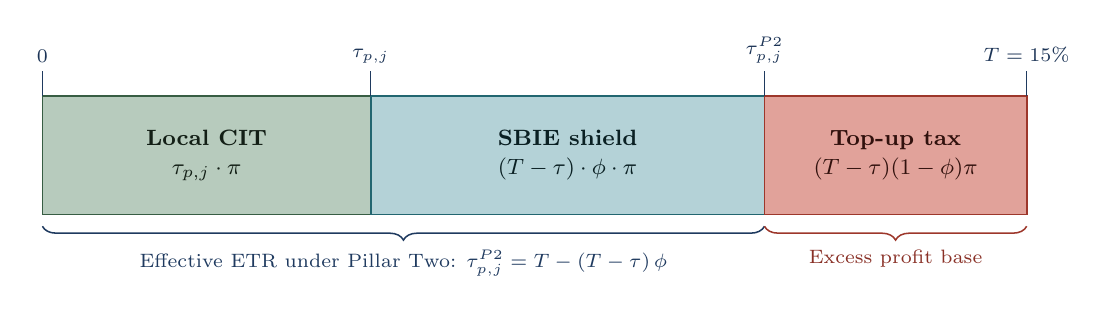
\begin{tikzpicture}[font=\small]
  % Bar dimensions
  \def\W{12.5}
  \def\H{1.5}
  % Sub-widths (proportional to a scenario with tau = 5% of profit-base, T = 15%, phi = 0.6)
  % local CIT = tau/T part of total potential tax = 5/15 = 1/3 of bar
  % gap = (T-tau) = 10/15 = 2/3 of bar; of which phi=0.6 → SBIE shielded; (1-phi)=0.4 → top-up
  % Use proportional widths: local CIT = 4.17 cm, SBIE = 5.0 cm, top-up = 3.33 cm  (sums to 12.5)
  \def\xa{4.17}
  \def\xb{9.17}

  % Background
  \fill[thesisLight] (0,0) rectangle (\W,\H);

  % Local CIT
  \fill[thesisGreen!40, draw=thesisGreen!75!black, line width=0.6pt] (0,0) rectangle (\xa, \H);
  \node[font=\footnotesize, align=center, thesisGreen!25!black]
    at (\xa/2, \H/2) {\textbf{Local CIT}\\[1pt]$\tau_{p,j}\cdot\pi$};

  % SBIE shield
  \fill[thesisTeal!35, draw=thesisTeal!80!black, line width=0.6pt] (\xa,0) rectangle (\xb, \H);
  \node[font=\footnotesize, align=center, thesisTeal!25!black]
    at ({(\xa+\xb)/2}, \H/2) {\textbf{SBIE shield}\\[1pt]$(T-\tau)\cdot\phi\cdot\pi$};

  % Top-up tax
  \fill[thesisRed!50, draw=thesisRed!80!black, line width=0.6pt] (\xb,0) rectangle (\W, \H);
  \node[font=\footnotesize, align=center, thesisRed!25!black]
    at ({(\xb+\W)/2}, \H/2) {\textbf{Top-up tax}\\[1pt]$(T-\tau)(1-\phi)\pi$};

  % Top axis with markers
  \draw[thesisNavy, line width=0.5pt] (0, \H) -- (0, \H+0.32);
  \draw[thesisNavy, line width=0.5pt] (\xa, \H) -- (\xa, \H+0.32);
  \draw[thesisNavy, line width=0.5pt] (\xb, \H) -- (\xb, \H+0.32);
  \draw[thesisNavy, line width=0.5pt] (\W, \H) -- (\W, \H+0.32);
  \node[above, font=\scriptsize, thesisNavy!90!black] at (0, \H+0.30) {$0$};
  \node[above, font=\scriptsize, thesisNavy!90!black] at (\xa, \H+0.30) {$\tau_{p,j}$};
  \node[above, font=\scriptsize, thesisNavy!90!black] at (\xb, \H+0.30) {$\tau^{P2}_{p,j}$};
  \node[above, font=\scriptsize, thesisNavy!90!black] at (\W, \H+0.30) {$T = 15\%$};

  % Effective P2 brace
  \draw[decorate, decoration={brace, mirror, amplitude=5pt}, thesisNavy, line width=0.55pt]
    (0,-0.15) -- node[below=5pt, font=\scriptsize]
    {Effective ETR under Pillar Two: $\tau^{P2}_{p,j} = T - (T-\tau)\,\phi$} (\xb,-0.15);

  % Top-up brace
  \draw[decorate, decoration={brace, mirror, amplitude=5pt}, thesisRed!80!black, line width=0.55pt]
    (\xb,-0.15) -- node[below=5pt, font=\scriptsize, thesisRed!70!black] {Excess profit base} (\W,-0.15);
\end{tikzpicture}
\caption[Effective Pillar Two tax floor.]{Decomposition of taxable profit at the 15\% threshold for a low-tax MNE affiliate. Local corporate income tax (green) collects $\tau_{p,j}\cdot\pi$. The SBIE (teal) shields a fraction $\phi=\text{SBIE}/\pi$ of the gap to the headline rate, leaving only the residual (red) as the excess profit base on which the top-up tax of $(T-\tau)(1-\phi)\pi$ is levied. The Pillar Two effective tax rate $\tau^{P2}_{p,j}$ therefore lies strictly below the headline 15\% whenever physical substance is positive, with the gap widening for capital- and labour-intensive sectors.}
\label{fig:effective_floor}
\end{figure}

where $\phi_{p,j} \equiv \text{SBIE}_{p,j} / \pi_{p,j}$ is the SBIE-to-profit ratio.\footnote{The $\phi$ notation for the SBIE-to-profit ratio is introduced in this thesis. \citet{devereux2023} compute the ratio but do not assign it a symbol; \citet{schjelderup2024} work with absolute SBIE values. The ratio formulation makes the effective floor directly comparable across jurisdictions with different profit levels. The symbol $\phi$ is chosen to avoid confusion with $\rho$, which conventionally denotes a correlation coefficient in econometric reporting.} The effective tax rate under Pillar Two falls \emph{strictly below} the headline rate $T = 15\%$ whenever the SBIE is positive. The gap is larger when the pre-reform ETR is further below 15\% (larger $\delta^{\text{top}}$) and the SBIE-to-profit ratio is larger (larger $\phi$).

The SBIE for each bilateral pair is:
\begin{equation}\label{eq:sbie}
\text{SBIE}_{p,j,t} = \sigma_W(t) \cdot \hat{W}_{p,j,t} + \sigma_A(t) \cdot A_{p,j,t}
\end{equation}
The carve-out rates decline linearly over a ten-year transition period (2024--2033). The payroll carve-out $\sigma_W$ starts at 10\% in 2024 and falls by 0.5 percentage points per year to reach 5\% from 2033 onward. The tangible asset carve-out $\sigma_A$ starts at 8\% in 2024 and falls by approximately 0.3 percentage points per year to reach 5\% from 2033 onward. The factorial design estimates revenue at both endpoints of this transition. Factor 3 switches between initial carve-out rates ($\sigma_W = 0.10$, $\sigma_A = 0.08$) and long-run rates ($\sigma_W = \sigma_A = 0.05$).

The payroll component $\hat{W}_{p,j,t}$ is a wage-based proxy rather than an observed CbCR quantity.\label{sec:payroll_imputation} Public CbCR does not report payroll: the only monetary labour-cost-like variable is \code{EARNINGS}, and OECD documentation of the CbCR template defines this measure as accumulated retained earnings rather than current-period compensation \citep{oecd2025a}. Treating \code{EARNINGS} as payroll would therefore introduce a measurement error at the level of the variable definition, not at the level of reporting quality. The base panel resolves this by constructing the SBIE payroll input directly as $\hat{W}_{p,j,t} = N_{p,j,t} \cdot \bar{w}_{j,t}$, the product of the CbCR Panel A-II (with Panel A-I and the panel-agnostic aggregate as sequential fall-backs) employee count and the affiliate-year wage benchmark described in Section \ref{sec:supplementary}. For Panel A-II coverage this procedure is almost complete in 2017--2022: a wage benchmark is matched for 14{,}685 of 16{,}915 pair-year cells, and the final wage-based payroll proxy is available for 14{,}610 cells. Missing payroll cells concentrate in small jurisdictions with neither CbCR employee coverage nor an OECD/ILO wage observation.

\subsubsection{SBTI Safe Harbour amplification}\label{sec:sbti_amplification}\label{sec:sbti}

The January 2026 OECD Administrative Guidance introduced the Substance-Based Tax Incentive (SBTI) Safe Harbour, which creates a second channel through which physical substance reduces the GMT burden \citep{oecd2026}. Under the original GloBE rules, local tax credits mechanically reduced covered taxes, driving the ETR below 15\% and triggering a top-up tax. The SBTI reverses this: MNEs may treat ``Qualifying Tax Incentives'' (QTIs; expenditure-based R\&D credits, volume-based production incentives) as an addition to covered taxes rather than a reduction. By inflating the ETR numerator, the safe harbour prevents the ETR from being artificially depressed.\footnote{The original GloBE design intended covered taxes to reflect the actual tax burden. Tax credits, even those designed to incentivise real economic activity, mechanically reduced covered taxes below the amount the jurisdiction intended the MNE to pay. The SBTI corrects this misalignment by treating qualifying incentives as additions to rather than reductions of covered taxes, preserving the incentive the source country offered.}

The benefit is bounded by a Substance Cap, for which two methods are available \citep{oecd2026}. Under Method 1 (the default, permanent option), the cap equals 5.5\% of the greater of eligible payroll costs or depreciation and depletion of eligible tangible assets:
\begin{equation}\label{eq:substance_cap}
\text{SC}_{p,j,t}^{\text{M1}} = 0.055 \times \max\!\left(\hat{W}_{p,j,t},\; \text{Depr}(A_{p,j,t})\right)
\end{equation}
where $\text{Depr}(A)$ denotes depreciation and depletion of eligible tangible assets. Under Method 2 (an elective alternative available for a five-year period), the cap equals 1\% of the carrying value of eligible tangible assets:
\begin{equation}\label{eq:substance_cap_m2}
\text{SC}_{p,j,t}^{\text{M2}} = 0.01 \times A_{p,j,t}
\end{equation}
MNEs elect whichever method yields the larger cap. Method 2 is designed for incentives linked to initial capital expenditure, where the carrying value provides greater relief in early years of asset life than depreciation.\footnote{If an MNE revokes a Method 2 election, assets previously included under Method 2 must be excluded from the depreciation calculation under Method 1, preventing double benefit. See \citet{oecd2026}, Chapter 1, Section 4.}

The SBTI and the SBIE rely on the \emph{same} macroeconomic variables: payroll and tangible assets. The SBIE reduces the denominator of the excess profit base; the SBTI inflates the numerator of the ETR. Capital-intensive sectors benefit doubly: larger SBIE carve-outs \emph{and} higher Substance Caps, allowing them to retain local tax incentives without triggering top-up taxes. Asset-light holding companies in conduit jurisdictions cannot utilise the SBTI because their payroll and tangible assets approach zero, driving the Substance Cap to zero.\footnote{The SBTI also has implications for tax competition. As \citet{janeba2023} predict, competition shifts from headline statutory rates toward opaque subsidies and qualified refundable tax credits. The SBTI explicitly protects expenditure-based incentives up to the Substance Cap, restricting effective tax competition to jurisdictions with heavy industrial footprints.}

Under the SBTI, the effective ETR becomes:
\begin{equation}\label{eq:etr_sbti}
\tau_{p,j}^{\text{SBTI}} = \frac{\theta_{p,j} + \min\!\left(\text{QTI}_{p,j},\; \max\!\left(\text{SC}_{p,j}^{\text{M1}},\; \text{SC}_{p,j}^{\text{M2}}\right)\right)}{\pi_{p,j}}
\end{equation}
where the MNE elects the method that yields the larger cap.

Public CbCR does not observe actual QTI claims. The measurement framework therefore cannot measure the SBTI benefit directly but can measure how much \emph{room} a jurisdiction--sector cell has to protect local tax incentives under the safe harbour. The Substance Cap sets the upper bound on the SBTI benefit; the SBTI-capacity proxy normalises this cap by profit to obtain a ratio comparable across jurisdictions and sectors:
\begin{equation}\label{eq:sbti_capacity}
\kappa_{j,s,t} = \frac{\max\!\left(0.055\,W_{j,s,t},\; 0.01\,A_{j,s,t}\right)}{\pi_{j,s,t}}
\end{equation}
The numerator approximates the maximum Substance Cap an MNE could claim from the two components that public data can construct. Under Method 1, the cap is $0.055 \times \max(W, \text{Depr}(A))$. CbCR reports neither eligible payroll nor depreciation. The Method 1 payroll arm is therefore reconstructed using the wage-based proxy $\hat{W}_{j,s,t}$ introduced in Section \ref{sec:payroll_imputation}, and the Method 1 asset arm cannot be computed from public data. The index takes the maximum of the Method 1 payroll arm ($0.055 \times \hat{W}$, reconstructed) and the Method 2 carrying-value cap ($0.01 \times A$, observed in CbCR \code{ASSETS}). It is an exposure measure. A high $\kappa$ indicates that a sector has substantial physical substance relative to profits and could therefore protect a large share of local tax incentives through the SBTI; a low $\kappa$ (characteristic of asset-light holding and IP licensing sectors) means the Substance Cap approaches zero and the SBTI provides little relief. The index enters the factorial design as part of the substance overlay in Factor 2 (Section \ref{sec:factors}).


\subsubsection{Sectoral decomposition}\label{sec:sbie_decomp}

A country-level SBIE ratio hides the fact that the carve-out is generous for manufacturing and almost nothing for a holding company. Because the GMT applies affiliate by affiliate, a country average for the substance shield can systematically over- or under-state protection depending on which sectors host the low-taxed profit. The sectoral decomposition of this subsection corrects for that mismatch by breaking the country-level substance shield down into sector-by-sector components. The aggregate SBIE-to-profit ratio $\phi$ masks substantial sectoral heterogeneity. Manufacturing subsidiaries have high payroll and tangible asset intensity relative to profits, generating SBIE ratios that can exceed 100\% of pre-tax profit; holding and IP licensing entities have near-zero substance, driving the SBIE toward zero \citep{devereux2023}. Since the GMT applies the top-up tax at the entity level, the aggregate $\phi$ overstates shielding for jurisdictions where low-taxed profit is concentrated in asset-light entities. The sectoral decomposition combines CbCR aggregate levels with the Eurostat FATS sectoral shares introduced in Section \ref{sec:sectoral_data}.

The SBIE-to-profit ratio $\phi$ depends on the composition of economic activity. Decomposing affiliates in jurisdiction $j$ into sectors $s \in \{1, \ldots, S\}$:

\begin{equation}\label{eq:rho_sectoral}
\phi_j = \sum_s \omega_{j,s} \cdot \phi_{j,s}, \quad \text{where } \omega_{j,s} = \frac{\pi_{j,s}}{\pi_j}
\end{equation}

and the sector-specific SBIE-to-profit ratio is:
\begin{equation}\label{eq:rho_sector}
\phi_{j,s} = \sigma_W \cdot \frac{W_{j,s}}{\pi_{j,s}} + \sigma_A \cdot \frac{A_{j,s}}{\pi_{j,s}}
\end{equation}

The effective tax floor for sector $s$ in jurisdiction $j$ is:
\begin{equation}\label{eq:floor_sector}
\tau_{j,s}^{\text{floor}} = T - (T - \tau_j) \cdot \phi_{j,s}
\end{equation}

CbCR does not report by sector. The sectoral decomposition combines CbCR aggregate levels with Eurostat FATS sectoral shares:
\begin{equation}\label{eq:sbie_sectoral}
\widehat{\text{SBIE}}_{j,s} = \sigma_W \cdot \left(\frac{\text{PersC}_{j,s}^{\text{FATS}}}{\sum_{s'} \text{PersC}_{j,s'}^{\text{FATS}}}\right) \cdot W_j^{\text{CbCR}} + \sigma_A \cdot \left(\frac{\hat{K}_{j,s}}{\sum_{s'} \hat{K}_{j,s'}}\right) \cdot A_j^{\text{CbCR}}
\end{equation}
\begin{figure}[H]
\centering
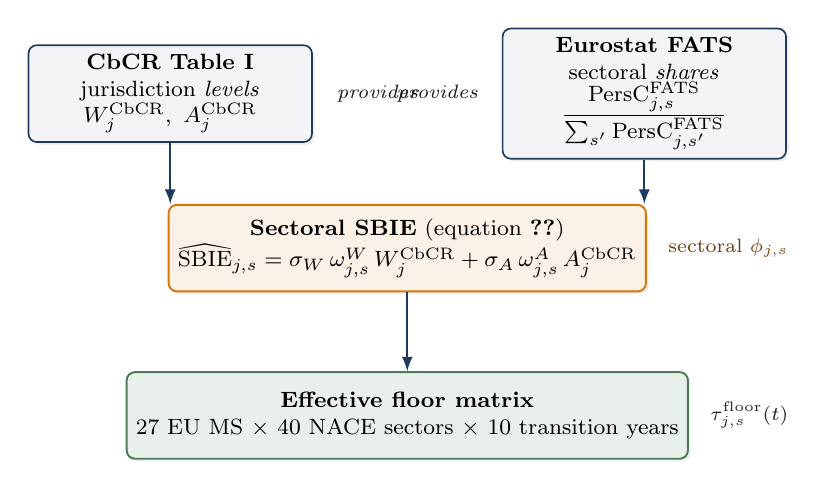
\begin{tikzpicture}[font=\small,
   src/.style={draw=thesisNavy, line width=0.6pt, rounded corners=3pt, fill=thesisLight,
               minimum width=3.6cm, minimum height=1.0cm, align=center, font=\footnotesize,
               drop shadow={shadow xshift=1pt, shadow yshift=-1pt, opacity=0.12}},
   prod/.style={draw=thesisOrange, line width=0.7pt, rounded corners=3pt,
                fill=thesisOrange!10, minimum width=4.6cm, minimum height=1.1cm,
                align=center, font=\footnotesize,
                drop shadow={shadow xshift=1pt, shadow yshift=-1pt, opacity=0.12}}]

  % Top row: sources
  \node[src] (cbcr) {\textbf{CbCR Table I}\\jurisdiction \emph{levels}\\$W^{\text{CbCR}}_j,\ A^{\text{CbCR}}_j$};
  \node[src, right=2.4cm of cbcr] (fats) {\textbf{Eurostat FATS}\\sectoral \emph{shares}\\$\dfrac{\text{PersC}^{\text{FATS}}_{j,s}}{\sum_{s'}\text{PersC}^{\text{FATS}}_{j,s'}}$};

  % Middle: combine box
  \node[prod, below=1.4cm of $(cbcr)!0.5!(fats)$] (combine)
    {\textbf{Sectoral SBIE} (equation \ref{eq:sbie_sectoral})\\
     $\widehat{\text{SBIE}}_{j,s}
        = \sigma_W\,\omega^{W}_{j,s}\,W^{\text{CbCR}}_j
        + \sigma_A\,\omega^{A}_{j,s}\,A^{\text{CbCR}}_j$};

  % Bottom: matrix output
  \node[prod, below=1.0cm of combine, fill=thesisGreen!12, draw=thesisGreen] (out)
    {\textbf{Effective floor matrix}\\
     27 EU MS\ \(\times\)\ 40 NACE sectors\ \(\times\)\ 10 transition years};

  % Arrows
  \draw[thesis arrow] (cbcr.south) -- ($(combine.north -| cbcr.south)$);
  \draw[thesis arrow] (fats.south) -- ($(combine.north -| fats.south)$);
  \draw[thesis arrow] (combine) -- (out);

  % Side annotations
  \node[font=\scriptsize\itshape, thesisGrey!20!black, anchor=west] at ($(cbcr.east) + (0.18,0)$) {provides};
  \node[font=\scriptsize\itshape, thesisGrey!20!black, anchor=east] at ($(fats.west) + (-0.18,0)$) {provides};
  \node[font=\scriptsize, thesisOrange!50!black, anchor=west] at ($(combine.east) + (0.15,0)$)
    {sectoral $\phi_{j,s}$};
  \node[font=\scriptsize, thesisGreen!30!black, anchor=west] at ($(out.east) + (0.15,0)$)
    {$\tau^{\text{floor}}_{j,s}(t)$};

\end{tikzpicture}
\caption[CbCR$\,\times\,$FATS and EUKLEMS construction of sectoral SBIE.]{Construction of the sectoral SBIE and the effective tax floor matrix. CbCR Table I provides the in-scope MNE \emph{levels} of payroll and tangible assets for each affiliate jurisdiction; Eurostat FATS provides the foreign-control cross-sectoral payroll and profit-proxy shares; EUKLEMS \& INTANProd provides the stock-based tangible-capital allocation where sectoral coverage is adequate. Their combination yields a sector-specific SBIE estimate $\widehat{\text{SBIE}}_{j,s}$ (equation \ref{eq:sbie_sectoral}), from which the effective tax floor $\tau^{\text{floor}}_{j,s}(t)$ is computed for each year of the SBIE transition.}
\label{fig:cbcr_fats_combo}
\end{figure}

where $\text{PersC}_{j,s}^{\text{FATS}}$ is personnel costs for sector $s$ in FATS and $\hat{K}_{j,s}$ is the selected tangible-capital allocator from the hierarchy in Table \ref{tab:sectoral_bridge_hierarchy}. FATS and EUKLEMS provide the \emph{sectoral shares}; CbCR provides the \emph{aggregate levels}. This is a transparent reweighting assumption, not direct sectoral GloBE measurement. The CbCR in-scope population (\EUR750 million+ MNEs) is a subset of the FATS population (all foreign-controlled enterprises), and the sectoral bridge is therefore a sensitivity layer whose validity depends on whether foreign-controlled sector shares approximate in-scope MNE sector shares inside each EU host country.\footnote{FATS does not report tangible assets directly. The revised implementation uses EUKLEMS \code{K\_Tang} stock shares where country-sector coverage is adequate. If EUKLEMS covers at least 75\% of the FATS turnover in a country-year, missing stock cells are gap-filled with FATS investment scaled by the observed stock-to-investment ratio in that country-year. If coverage is weaker, the whole country-year falls back to FATS gross investment. The sectoral profit proxy uses positive FATS gross operating surplus where available, then value added, and turnover only as a last fallback.}

The Eurostat inward FATS underwent a structural break in 2021: the pre-2021 series (\code{fats\_g1b\_08}) uses a single broad aggregate and 23 indicators, while the post-2021 series (\code{fats\_activ}) uses 48 NACE-based activity categories and 19 \code{indic\_sbs} codes. The sectoral estimation therefore uses post-2021 \code{fats\_activ} data only.

The effective tax floor evolves over the SBIE transition period (2024--2033):
\begin{equation}\label{eq:floor_transition}
\tau_{j,s}^{\text{floor}}(t) = T - (T - \tau_j) \cdot \left[\sigma_W(t) \cdot \frac{W_{j,s}}{\pi_{j,s}} + \sigma_A(t) \cdot \frac{A_{j,s}}{\pi_{j,s}}\right]
\end{equation}
The output is a matrix of effective tax floors: 27 EU Member States $\times$ 40 non-overlapping NACE sectors $\times$ 10 transition years.

For jurisdictions where the ETR distribution straddles $T$, the aggregate $\phi_j$ overstates the effective shielding of the GMT base if high-ETR entities are disproportionately capital-intensive. The SBIE reduces the top-up tax only on the low-taxed portion, not on entities already above $T$. Table IV's activity composition variables (\code{ACT\_HOLDING}, \code{ACT\_IP}, \code{ACT\_MAN}) for the \code{RATE\_0-15} bracket reveal whether low-taxed profit is concentrated in holding/IP activities (low $\phi$, suggesting proportional SBIE allocation \emph{overstates} shielding) or in manufacturing (high $\phi$, suggesting it \emph{understates} shielding). The sensitivity analysis tests both extremes.

This subsection delivers the SBIE filter $(1 - \bar{\phi}_{p,j,t})$: the fraction of low-taxed profit that constitutes excess profit and is subject to the top-up tax. The factorial design varies this filter through two factors: Factor 2 switches between the aggregate CbCR-based $\phi$ and the sectoral FATS-based $\phi$ with SBTI-capacity overlay, and Factor 3 switches between initial and long-run carve-out rates.

\newpage

\section{Methodology}\label{sec:methodology}

The methodology starts from the measured objects constructed in Section \ref{sec:data}: corrected profit $\pi^{*}_{p,j,t}$, low-taxed profit $\ell_{p,j,t}$, the average top-up rate $\bar{\delta}_{j,t}^{\text{top}}$, the SBIE shield $\bar{\phi}_{p,j,t}$, and legal allocation indicators. It estimates the behavioural semi-elasticity of reported profits, maps that estimate into a counterfactual reallocation factor, allocates the resulting liability under the QDMTT/IIR/UTPR rule order, and decomposes the revenue spread across the remaining modelling choices.

The baseline econometric model is a Hines--Rice panel regression with parent--affiliate fixed effects and year fixed effects. The robustness layer is deliberately separated by purpose. Alternative samples test whether the estimated tax response is sensitive to panel expansion, stale wage inputs or pandemic-year profit compression. The tax-code IV diagnostics evaluate whether current CbCR ETRs contain endogenous profit-shifting variation by comparing an OECD simulated effective-rate instrument with a lagged statutory-rate benchmark. The lower-tail support diagnostic asks whether the low-ETR region that drives the behavioural counterfactual is empirically supported, and the jurisdiction-influence exercise asks whether the final revenue decomposition depends on one dominant parent or affiliate jurisdiction.

\subsection{Panel estimation of profit-shifting semi-elasticities}\label{sec:estimation}

Before modelling how firms react to the reform, the thesis needs a number for how sensitive reported profits are to tax rates. That number is the tax semi-elasticity of reported profits. This section estimates it directly from the 2017--2022 CbCR panel, so that the behavioural counterfactual inherits the standard errors and the functional-form uncertainty of its own estimation step. Published semi-elasticities are estimated either from US-only data \citep{dowd2017} or from a single cross-section of OECD CbCR \citep{garcia-bernardo2024}. The panel structure of this thesis provides two identification advantages: within-pair variation across six fiscal years, which absorbs time-invariant bilateral confounders, and sufficient degrees of freedom to compare functional forms with formal specification tests rather than visual inspection.

\subsubsection{Estimation framework}\label{sec:hines_rice}

The estimation follows the Hines--Rice framework \citep{hines1994}, as extended by \citet{garcia-bernardo2024}. Reported pre-tax profit in affiliate jurisdiction $j$ of parent $p$ in year $t$ is modelled as a function of real economic activity and the tax incentive to shift profits:
\begin{equation}\label{eq:panel_linear}
\log \pi_{p,j,t}^{*} = \beta_0 + \beta_1 \log A_{p,j,t} + \beta_2 \log \hat{W}_{p,j,t} + \beta_3 \, \tau_{p,j,t} + \mathbf{\beta}_x \mathbf{X}_{p,j,t} + \alpha_{pj} + \gamma_t + \varepsilon_{p,j,t}
\end{equation}
where $\pi^{*}$ is corrected profit (Section \ref{sec:doublecounting}), $A$ is tangible assets, $\hat{W}$ is the wage-based payroll proxy (Section \ref{sec:payroll_imputation}), $\tau$ is the effective tax rate, $\alpha_{pj}$ is a parent--affiliate pair fixed effect, and $\gamma_t$ is a year fixed effect. The vector $\mathbf{X}$ contains log GDP per capita and log population of the affiliate jurisdiction.\footnote{Tangible assets $A$ are themselves affected by profit shifting: US MNEs in Luxembourg report the second-highest value of tangible assets in Europe \citep{garcia-bernardo2024}. Using tangible assets as a control therefore produces conservative semi-elasticity estimates, since part of the profit-shifting effect is absorbed by the capital stock. The endogeneity of $\tau$ is addressed separately through the tax-code IV diagnostics below.} The coefficient $\beta_3$ is the linear semi-elasticity: the percentage change in reported profits for a one percentage-point change in the ETR.\footnote{The bilateral pair fixed effects $\alpha_{pj}$ absorb all time-invariant determinants of bilateral profit allocation: treaty networks, geographic and linguistic proximity, legal system similarity, and persistent features of MNE group structure. Identification of $\beta_3$ therefore comes from \emph{within-pair} variation in ETRs over 2017--2022, driven partly by tax reforms and partly by changes in reporting composition and profit bases. Year fixed effects absorb global shocks (the 2017 TCJA, the 2020 COVID contraction, and the post-2020 recovery).}

Following \citet{dowd2017} the quadratic specification is estimated:
\begin{equation}\label{eq:panel_quadratic}
\log \pi_{p,j,t}^{*} = \beta_0 + \beta_1 \log A_{p,j,t} + \beta_2 \log \hat{W}_{p,j,t} + \beta_3 \, \tau_{p,j,t} + \beta_4 \, \tau_{p,j,t}^2 + \mathbf{\beta}_x \mathbf{X}_{p,j,t} + \alpha_{pj} + \gamma_t + \varepsilon_{p,j,t}
\end{equation}
The implied semi-elasticity varies with the ETR: $\varepsilon(\tau) = \beta_3 + 2\beta_4 \tau$.

Following \citet{garcia-bernardo2024} also the logarithmic specification is estimated:
\begin{equation}\label{eq:panel_log}
\log \pi_{p,j,t}^{*} = \beta_0 + \beta_1 \log A_{p,j,t} + \beta_2 \log \hat{W}_{p,j,t} + \beta_3 \, \tau_{p,j,t} + \beta_4 \log(t_0 + \tau_{p,j,t}) + \mathbf{\beta}_x \mathbf{X}_{p,j,t} + \alpha_{pj} + \gamma_t + \varepsilon_{p,j,t}
\end{equation}
where $t_0$ is a small offset parameter selected by minimising the BIC over the grid $t_0 \in [0.001, 0.200]$.\footnote{The offset $t_0$ prevents the logarithm from diverging at $\tau = 0$ and governs how steeply the semi-elasticity rises at very low ETRs. \citet{garcia-bernardo2024} report $t_0 = 0.0023$ based on the 2017 CbCR panel. The panel estimate may differ because the time dimension introduces additional variation at the tails.} The implied semi-elasticity is $\varepsilon(\tau) = \beta_3 + \beta_4 / (t_0 + \tau)$, which rises sharply as $\tau \to 0$. This is the key feature that captures extreme profit shifting at near-zero ETRs.\footnote{The logarithmic specification implies that the semi-elasticity becomes unbounded as $\tau \to 0$. In the revenue simulation, this is bounded by the data: the lowest observed ETR percentile (P5) provides a natural floor. Counterfactual profit changes are winsorised at the 99th percentile of the estimated $\hat{\beta}_{j,t}$ distribution to prevent a small number of cells with near-zero P5 from dominating the aggregate.}

\begin{figure}[H]
\centering
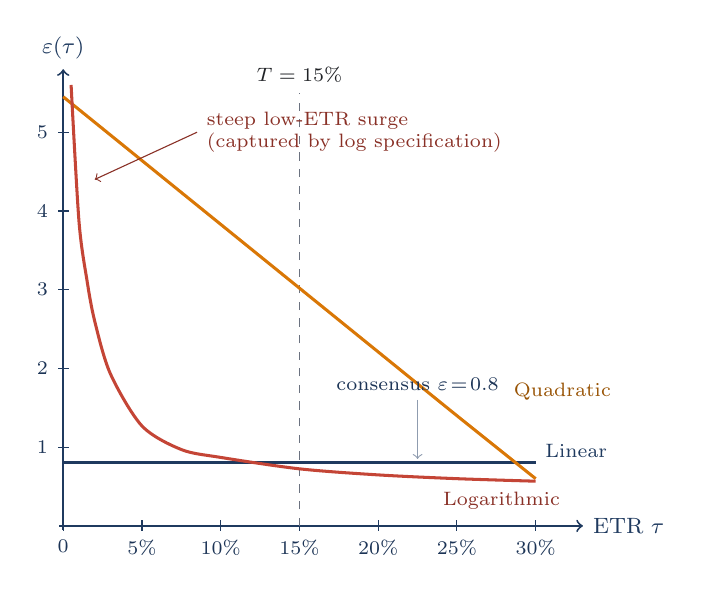
\begin{tikzpicture}[font=\small]
  % Coordinate system: x = tau in [0,30%]; we map x*20cm so 0.30 -> 6cm
  % y = semi-elasticity in [0, 5.5]; we map y*1cm
  \def\xmax{6.6}
  \def\ymax{5.8}

  % Axes
  \draw[->, thesisNavy, line width=0.7pt] (-0.05,0) -- (\xmax,0) node[right, font=\footnotesize] {ETR $\tau$};
  \draw[->, thesisNavy, line width=0.7pt] (0,-0.05) -- (0,\ymax) node[above, font=\footnotesize] {$\varepsilon(\tau)$};

  % x ticks (5% intervals)
  \foreach \xv/\lbl in {0/0, 1/{5\%}, 2/{10\%}, 3/{15\%}, 4/{20\%}, 5/{25\%}, 6/{30\%}} {
    \draw[thesisNavy] (\xv, 0.07) -- (\xv, -0.07);
    \node[below, font=\scriptsize, thesisNavy!90!black] at (\xv, -0.05) {\lbl};
  }
  % y ticks
  \foreach \yv in {1,2,3,4,5} {
    \draw[thesisNavy] (0.07, \yv) -- (-0.07, \yv);
    \node[left, font=\scriptsize, thesisNavy!90!black] at (-0.07, \yv) {\yv};
  }

  % T = 15% reference line
  \draw[dashed, thesisGrey, line width=0.6pt] (3, 0) -- (3, 5.5);
  \node[font=\scriptsize, thesisGrey!30!black, anchor=south] at (3, 5.5) {$T = 15\%$};

  % Linear: epsilon = 0.8
  \draw[thesisNavy, line width=1.1pt] (0, 0.8) -- (6, 0.8);
  \node[font=\scriptsize, thesisNavy, anchor=west] at (6.0, 0.95) {Linear};

  % Quadratic Dowd: epsilon(tau) = -10.73 + 16.178*(1 - tau)
  \draw[thesisOrange, line width=1.1pt]
    plot[smooth] coordinates {(0,5.45) (1,4.64) (2,3.83) (3,3.02) (4,2.21) (5,1.40) (6,0.60)};
  \node[font=\scriptsize, thesisOrange!70!black, anchor=west] at (5.6, 1.7) {Quadratic};

  % Logarithmic: epsilon(tau) = b3 + b4 / (t0 + tau), illustrative parameters
  \draw[thesisRed, line width=1.1pt]
    plot[smooth] coordinates {(0.1,5.6) (0.2,3.87) (0.3,3.13) (0.4,2.6) (0.6,1.93)
      (1,1.27) (1.5,0.97) (2,0.87) (3,0.725) (4,0.648) (5,0.6) (6,0.568)};
  \node[font=\scriptsize, thesisRed!70!black, anchor=west] at (4.7, 0.32) {Logarithmic};

  % Annotation: meta-regression consensus
  \draw[thesisNavy!50, ->, line width=0.4pt] (4.5, 1.6) -- (4.5, 0.85);
  \node[font=\scriptsize, thesisNavy!90!black, anchor=south] at (4.5, 1.6) {consensus $\varepsilon\!=\!0.8$};

  % Annotation: nonlinear surge at low ETRs
  \draw[thesisRed!70!black, ->, line width=0.4pt] (1.7, 5) -- (0.4, 4.4);
  \node[font=\scriptsize, thesisRed!70!black, anchor=west, align=left] at (1.7, 5)
    {steep low-ETR surge\\(captured by log specification)};
\end{tikzpicture}
\caption[Implied semi-elasticity under three functional forms.]{Implied profit-shifting semi-elasticity $\varepsilon(\tau)$ under the three functional forms compared in Section \ref{sec:hines_rice}: the linear specification, equivalent to the meta-regression consensus of \citet{heckemeyer2017}; the quadratic specification of \citet{dowd2017} estimated on US administrative tax-return data; and the logarithmic specification of \citet{garcia-bernardo2024} estimated on a 2017 OECD CbCR cross-section. Coefficient values are illustrative; the panel-estimated values are reported in Section \ref{sec:se_results}. The vertical dashed line marks the GMT threshold $T=15\%$. The logarithmic specification accommodates an unbounded surge in profit responsiveness as the ETR approaches zero, the regime in which the GMT base is concentrated.}
\label{fig:semi_elasticity_forms}
\end{figure}

\subsubsection{Identification}\label{sec:identification}

The pair fixed effects $\alpha_{pj}$ absorb all time-invariant bilateral determinants of profit allocation. Identification of the semi-elasticity coefficients ($\beta_3$, and $\beta_4$ where applicable) relies on within-pair changes in the effective tax rate over 2017--2022. Some of this variation is plausibly policy-driven: several EU Member States reduced their headline CIT rates during this period (e.g.\ France from 33.3\% to 25\%, Belgium from 33.99\% to 25\%), and the 2017 US Tax Cuts and Jobs Act reduced the US federal CIT rate from 35\% to 21\% while introducing GILTI. But the CbCR ETR is not a statutory variable. It is tax accrued divided by reported profit, so it also moves when the composition of reporting entities changes, when loss carry-forward mechanics alter the tax numerator, or when MNEs shift profit into the denominator. The fixed-effect model therefore improves on the cross-section but does not by itself solve tax endogeneity. The IV diagnostics below are included to quantify how much of the tax variation is traceable to external tax-code changes.

The sufficiency of within-pair ETR variation is an empirical question. Section \ref{sec:descriptive} reports the within-pair standard deviation of ETR. If the median within-pair standard deviation falls below 2 percentage points, the fixed-effects estimator may lack power relative to a specification that also uses between-pair variation. In that event, correlated random effects specification is estimated as an alternative: it augments the pooled regression with the pair-level mean of each time-varying regressor, so the coefficient on the demeaned regressor identifies the within-pair effect while the coefficient on the mean captures the between-pair effect.

\subsubsection{Instrumental-variable robustness}\label{sec:iv_strategy}

There is an endogeneity concern. The CbCR ETR is computed as tax accrued divided by profit before tax. If an MNE shifts profit into an affiliate jurisdiction, the denominator of $\tau_{p,j,t}$ changes at the same time as the dependent variable $\log \pi^{*}_{p,j,t}$. OLS can therefore mix the tax response with reverse causality from the accounting identity itself. To isolate tax variation that is not mechanically created by current-year reported profit, the preferred IV diagnostic uses the OECD forward-looking effective average tax rate for a fixed composite investment project in affiliate jurisdiction $j$ and year $t$, denoted $z_{j,t}^{\text{sim}}$. This simulated EATR holds the investment project fixed and varies the tax-code environment: statutory rates, allowances and other rules embedded in the OECD forward-looking tax model. It is therefore closer to the simulated-instrument logic than the raw statutory rate. The one-year lagged statutory CIT rate, $z_{j,t-1}^{\text{CIT}}$, is retained as a benchmark because it is predetermined but less closely tied to the effective tax base.

The first stage is:
\begin{equation}\label{eq:iv_first_stage}
\tau_{p,j,t} = \pi_0 + \pi_1 z_{j,t}^{\text{IV}} + \pi_2 \log A_{p,j,t} + \pi_3 \log \hat{W}_{p,j,t} + \mathbf{\pi}_x \mathbf{X}_{j,t} + \alpha_{pj} + \gamma_t + \nu_{p,j,t},
\end{equation}
where $z_{j,t}^{\text{IV}}$ is estimated separately as $z_{j,t}^{\text{sim}}$ and $z_{j,t-1}^{\text{CIT}}$.
The second stage replaces the potentially endogenous CbCR ETR in the linear Hines--Rice equation with the first-stage fitted value:
\begin{equation}\label{eq:iv_second_stage}
\log \pi_{p,j,t}^{*} = \beta_0^{\text{IV}} + \beta_1^{\text{IV}} \log A_{p,j,t} + \beta_2^{\text{IV}} \log \hat{W}_{p,j,t} + \beta_3^{\text{IV}} \widehat{\tau}_{p,j,t} + \mathbf{\beta}_x^{\text{IV}} \mathbf{X}_{j,t} + \alpha_{pj} + \gamma_t + \varepsilon_{p,j,t}^{\text{IV}}.
\end{equation}
The reduced form is estimated in parallel by replacing $\tau_{p,j,t}$ in \eqref{eq:iv_second_stage} with each excluded instrument. This is informative because a strong first stage without a same-signed reduced form would not support a strong causal interpretation of the IV coefficient.

The identifying assumption remains a concern. The simulated EATR is external to the CbCR denominator and is based on a fixed investment project, but tax-code reforms may still respond to unobserved fiscal pressures or avoidance activity that also affect reported profits. The statutory benchmark is predetermined with respect to current-year accounting choices, but it ignores allowances and credits that move effective rates. The IV estimates are therefore treated as robustness diagnostics for the linear tax coefficient, not as the preferred estimator for the nonlinear counterfactual. Extending the IV design to the quadratic or logarithmic specifications would require separate excluded instruments for the nonlinear tax terms and a multivariate weak-instrument assessment, which the public CbCR panel cannot support credibly.

\subsubsection{Inference}\label{sec:inference}

The main regression table reports parent-and-affiliate two-way clustered standard errors, because residual correlation can run through the parent side of the CbCR reporting system as well as through common host-country tax shocks. Affiliate-clustered standard errors are retained as a one-way diagnostic, since all MNEs operating in Ireland, Luxembourg or the Netherlands face correlated affiliate-level tax and reporting shocks.\footnote{\citet{garcia-bernardo2024} use heteroscedasticity-robust standard errors on their cross-section; the panel structure here requires cluster-robust inference. Two-way clustering is the preferred presentation because the data are bilateral and both dimensions can generate dependence. The affiliate-clustered variant is reported to make the comparison with host-country tax shocks transparent.} Model selection proceeds in two stages. First, the BIC ranks the three functional forms. The BIC penalises model complexity more heavily than the AIC and is highly effective for comparing non-nested models with different numbers of parameters on the same sample. Second, because the quadratic and logarithmic specifications are non-nested (neither is a restricted case of the other), a \citet{vuong1989} test compares their observation-level log-likelihoods to determine whether one fits the data systematically better.

\subsubsection{Behavioural counterfactual response}\label{sec:counterfactual}

The estimated coefficients $(\hat{\beta}_3, \hat{\beta}_4)$ and the implied semi-elasticity curve $\hat{\varepsilon}(\tau)$ feed into the behavioural counterfactual, where they are mapped to an affiliate-year reallocation factor through the closed-form counterfactual ratios in equations \eqref{eq:cf_linear}--\eqref{eq:cf_log} and the Stage 1 low-taxed-slice ETR in \eqref{eq:beta_aggregated}.\footnote{The counterfactual holds tangible assets $A$ and payroll $\hat{W}$ at their pre-reform values. This is consistent with the evidence that real investment responds more slowly than profit allocation \citep{suarezserrato2018} and with the short- to medium-run horizon over which the semi-elasticity is identified. The second-round effect (SBIE shrinkage through reduced substance) is discussed in Section \ref{sec:limitations} but not modelled in the baseline.} Estimation uncertainty in $(\hat{\beta}_3, \hat{\beta}_4)$ is reported through the Stage 3 standard errors and would enter the revenue estimates through a coefficient-propagation exercise; it should not be conflated with the factorial behavioural scenario. Equation \eqref{eq:counterfactual_profit} records the generic ratio notation, while Section \ref{sec:reallocation_mapping} gives the implemented branch-specific mapping.

\begin{equation}\label{eq:counterfactual_profit}
\hat{\pi}^{\text{GMT}}(\tau) \;=\; \pi^{*} \cdot G_m(\tau) \quad \text{with } G_m(\tau) \text{ given by \eqref{eq:cf_linear}--\eqref{eq:cf_log}.}
\end{equation}

\subsubsection{Robustness}\label{sec:estimation_robustness}
Robustness is tested on two levels. The first level assesses the estimated semi-elasticity. The model comparison is repeated on a balanced six-year pair panel, after excluding affiliate-year wage proxies based on stale wage observations, and after excluding the 2020--2021 fiscal years. Standard errors are reported under affiliate clustering and parent-and-affiliate clustering, and the FE-2SLS diagnostics in equations \eqref{eq:iv_first_stage}--\eqref{eq:iv_second_stage} instrument the current CbCR ETR with the OECD simulated fixed-project EATR and, as a benchmark, the one-year lagged statutory CIT rate of the affiliate jurisdiction. These checks ask whether the behavioural parameter is sensitive to expanding CbCR coverage, wage-proxy quality, pandemic-year profit compression, cluster definition or mechanical ETR endogeneity.

A separate lower-tail support diagnostic assesses whether the nonlinear terms are credibly identified below an ETR of 5 per cent. Inverse probability weighting is not used as a primary estimator. In its standard treatment-effect use, IPW targets a population estimand by weighting observations with the inverse of an estimated propensity score \citep{hirano2003}. In the present CbCR setting, a below-5 per cent ETR is not an externally assigned treatment or a known sampling event. It is part of the tax-avoidance outcome whose behavioural response is being estimated. The pipeline therefore reports support counts, profit shares, within-pair switching support and an illustrative tail-balanced design. This answers the identification question without changing the estimand or relabelling arbitrary tail weights as IPW.

The second level assesses jurisdictional influence. Public CbCR is concentrated in a small number of parent and affiliate jurisdictions, so the pipeline now drops one jurisdiction at a time as parent and as affiliate. The named set is the United States, the Netherlands, Ireland, Luxembourg, Germany, France, Switzerland and Singapore; the suite also adds the largest high-profit jurisdictions in each dimension. For each omission, the code refits the Stage 3 semi-elasticity model, recomputes the profit-weighted Stage 1 liability rate, and rebuilds the final Stage 4.5--4.6 EU revenue decomposition. This is an influence diagnostic rather than an alternative point estimate: large jurisdictions are real parts of the tax base, so the full-sample estimate remains preferred, but a publishable estimate must disclose whether the conclusion depends on one jurisdiction.

\subsection{Behavioural counterfactual response}\label{sec:behavioural}

Once the minimum tax binds, the rate differential that drew profit into low-tax affiliates shrinks, and firms that shifted profit in the first place will shift less of it. The behavioural counterfactual enters the revenue equation \eqref{eq:pipeline} through the liability filter $m_{j,t}^{\text{beh}}$. Below the SESH bandwidth this filter equals $(1-\beta_{j,t})$, where $\beta_{j,t}$ is the cross-border reallocation share after measurement branch, legal-exposure and unit-interval restrictions. If the estimated $\beta_{j,t}$ is 0.3, then thirty per cent of the mechanically computed top-up base leaves the jurisdiction once firms adjust. Inside the SESH bandwidth the mechanism is different: profit remains in place, but the top-up liability is deemed zero if the simplified ETR reaches the threshold.

Two margins enter the filter. The first is the gradual shrinkage of reported profit in each low-tax affiliate once the marginal rate on the measured low-taxed slice rises to $T$; its size is governed by the semi-elasticity curve estimated in Section~\ref{sec:estimation} and by the Stage 1 top-up rate in \eqref{eq:tau_low_segment}. The second is a sharp bunching response at fifteen per cent created by the Simplified ETR Safe Harbour (SESH) introduced in the January 2026 Administrative Guidance. The two margins are disjoint by construction: bunching applies inside the narrow band just below the floor, semi-elasticity reallocation applies below that band.

The remaining subsections anchor the filter in the optimal-shifting model of \citet{johannesen2022}, integrate the estimated semi-elasticity curve into a jurisdiction--year reallocation factor, overlay the safe-harbour response, and locate the reallocated profit against the distribution of real activity.

The implementation separates the size of the behavioural response from the diagnostic description of where profit might be re-reported. The revenue matrix uses only the estimated semi-elasticity response in \eqref{eq:cf_linear}--\eqref{eq:cf_log}, the legal collection exposure under the universal or SbS regime, and the SESH notch in \eqref{eq:regime}. It does not multiply the estimated response by channel-specific planning scores, and it does not impose a discretionary cap below the logical unit-interval bound. This matters for publication: public CbCR can identify a reduced-form profit response to tax rates, but it does not observe whether the marginal euro moved through transfer pricing, licensing, debt finance or real activity relocation. Channel labels are therefore kept as diagnostic outputs only, anchored in the \citet{heckemeyer2017} distinction between transfer-pricing/licensing and financial-planning channels. Real substance relocation is excluded from the short-run behavioural filter because payroll and tangible assets are held fixed in the SBIE calculation.


\subsubsection{From semi-elasticity estimates to the reallocation factor}\label{sec:reallocation_mapping}

The reallocation factor $\hat{\beta}_{j,t}^{e,m}$ is the predicted share of measured low-taxed profit that leaves jurisdiction $j$ once the marginal rate on that low-taxed slice is raised to $T$. The superscript $e$ indexes the ETR measurement branch, average or distributional, and $m$ indexes the selected semi-elasticity model. This affiliate-year construction follows the implemented Stage 1 object: the pipeline measures the ETR of the profit slice that enters the GMT base at the affiliate-year level, then applies that response to bilateral parent--affiliate rows with positive post-SBIE top-up exposure.

Throughout this section $\hat{\beta}_3$ and $\hat{\beta}_4$ are the coefficients of \eqref{eq:panel_linear}--\eqref{eq:panel_log} with their natural regression signs: $\hat{\beta}_3<0$ in every specification; $\hat{\beta}_4>0$ in the quadratic specification and $\hat{\beta}_4<0$ in the logarithmic one. The semi-elasticity viewed as a positive magnitude is $\hat{\varepsilon}(\tau) \equiv -\partial \log \pi / \partial \tau > 0$.

Holding real activity fixed, define $G_m(\tau)$ as the counterfactual profit ratio implied by model $m$ when the relevant ETR rises from $\tau$ to the minimum rate $T$. For a generic ETR argument $\tau<T$, the fundamental theorem of calculus gives
\begin{equation}\label{eq:cf_integral}
\log G_m(\tau) \;=\; \int_{\tau}^{T} \frac{\partial \log \pi}{\partial s}\, \mathrm{d}s \;=\; -\int_{\tau}^{T} \hat{\varepsilon}_m(s)\,\mathrm{d}s.
\end{equation}
The integrand is positive, so the counterfactual ratio is strictly below one whenever $\tau<T$. Evaluating the integral under each functional form yields the closed-form ratios used directly in the simulation:
\begin{align}
\text{Linear:} \qquad & G_{\text{lin}}(\tau) \;=\; \exp\!\left[\hat{\beta}_3\,(T - \tau)\right], \label{eq:cf_linear}\\
\text{Quadratic:} \qquad & G_{\text{quad}}(\tau) \;=\; \exp\!\left[\hat{\beta}_3\,(T - \tau) + \hat{\beta}_4\,(T^2 - \tau^2)\right], \label{eq:cf_quad}\\
\text{Logarithmic:} \qquad & G_{\text{log}}(\tau) \;=\; \exp\!\left[\hat{\beta}_3\,(T - \tau) + \hat{\beta}_4\bigl(\log(t_0 + T) - \log(t_0 + \tau)\bigr)\right]. \label{eq:cf_log}
\end{align}
The logarithmic expression uses $\int \hat{\beta}_4 / (t_0 + s)\,\mathrm{d}s = \hat{\beta}_4 \log(t_0 + s)$ up to a constant. Equations \eqref{eq:cf_linear}--\eqref{eq:cf_log} supersede \eqref{eq:counterfactual_profit} and share its sign convention.\footnote{With $\hat{\beta}_3 < 0$ and $T > \tau$, the linear exponent is negative. In the logarithmic case $\hat{\beta}_4 < 0$ and $\log(t_0 + T) > \log(t_0 + \tau)$, so the second exponent term is also negative. In the quadratic case $\hat{\beta}_4 > 0$ and $T^2 - \tau^2 > 0$, so the second term is positive and partially offsets the first, producing the flatter response at higher $\tau$ that motivates the quadratic form.}

The implemented argument of $G_m(\cdot)$ is not the jurisdiction-average ETR itself. For each ETR measurement branch, Stage 1 supplies the profit-weighted average top-up rate on the low-taxed slice, $\bar{\delta}_{j,t}^{\text{top},e}$. The implied ETR of the profit that actually enters the GMT base is:
\begin{equation}\label{eq:tau_low_segment}
\tau_{j,t}^{\text{low},e} = T - \bar{\delta}_{j,t}^{\text{top},e}.
\end{equation}
Reallocation is active only when the branch identifies a positive low-taxed share and a positive top-up rate. The raw affiliate-year response is therefore:
\begin{equation}\label{eq:beta_aggregated}
\hat{\beta}_{j,t}^{e,m}
\;=\;
\mathbf{1}\{s_{j,t}^{<T,e}>0,\ \bar{\delta}_{j,t}^{\text{top},e}>0\}
\cdot \left[1-G_m\!\left(\tau_{j,t}^{\text{low},e}\right)\right],
\end{equation}
with the result bounded to the unit interval. In the final revenue matrix this static response is applied only to bilateral rows with positive post-SBIE low-taxed profit and legal collection exposure. QDMTT exposure leaves the behavioural response active, while an SbS-exempt parent in a source jurisdiction without a QDMTT sets the collection-exposure multiplier to zero. Inside the SESH bandwidth the response is not \eqref{eq:beta_aggregated}; the liability filter in \eqref{eq:regime} sets top-up tax to zero with no cross-border reallocation.

\subsubsection{Safe-harbour regime and bunching under the Simplified ETR Safe Harbour}\label{sec:bunching}\label{sec:sesh}

The Simplified ETR Safe Harbour (SESH) in the January 2026 Administrative Guidance creates a permanent simplified ETR route that generally applies for fiscal years commencing on or after 31 December 2026, with earlier availability from 31 December 2025 only in specified cases \citep{oecd2026}. The same package extends the Transitional CbCR Safe Harbour by one year to ease the move into the permanent SESH. An affiliate jurisdiction whose simplified ETR meets or exceeds fifteen per cent has its top-up tax deemed zero and avoids the full GloBE computation for that jurisdiction. The SESH therefore creates a behavioural margin distinct from cross-border reallocation: the target of the response is the simplified ETR itself, not the location of the underlying profit.

The SESH is structurally a \emph{notch}. Conditional on no other safe harbour applying, a simplified ETR just below fifteen per cent leaves the group in the full GloBE computation for that tested jurisdiction, while reaching fifteen per cent deems the top-up tax to be zero. The bunching literature on kinked and notched tax schedules predicts that taxpayers whose unconstrained ETR falls just below such a threshold will manage their way onto the favourable side of it. \citet{saez2010} derives the benchmark response at kinks, \citet{kleven2013} show how notches can identify both optimisation frictions and structural elasticities when post-notch density data are available, and \citet{kleven2016} summarises the broader bunching design. Figure~\ref{fig:sesh_bunching} sketches the expected density: a missing mass in the band just below fifteen per cent and a compensating spike at the threshold.

This is also where the public-data limit bites. A structural notch-bunching estimator needs an observed post-policy density, because the key empirical objects are excess mass at the threshold and missing mass in the strictly dominated region below it. The present CbCR panel ends in 2022, before the SESH can affect reported simplified ETRs. This thesis therefore implements only a pre-reform density diagnostic: it bins jurisdiction-year average ETRs, fits a polynomial counterfactual outside the excluded region around fifteen per cent, and reports placebo excess and missing mass. This is useful for showing how much pre-reform profit sits close to the threshold and for designing a later structural estimator, but it is not evidence that firms have already bunched.

\begin{figure}[H]
\centering
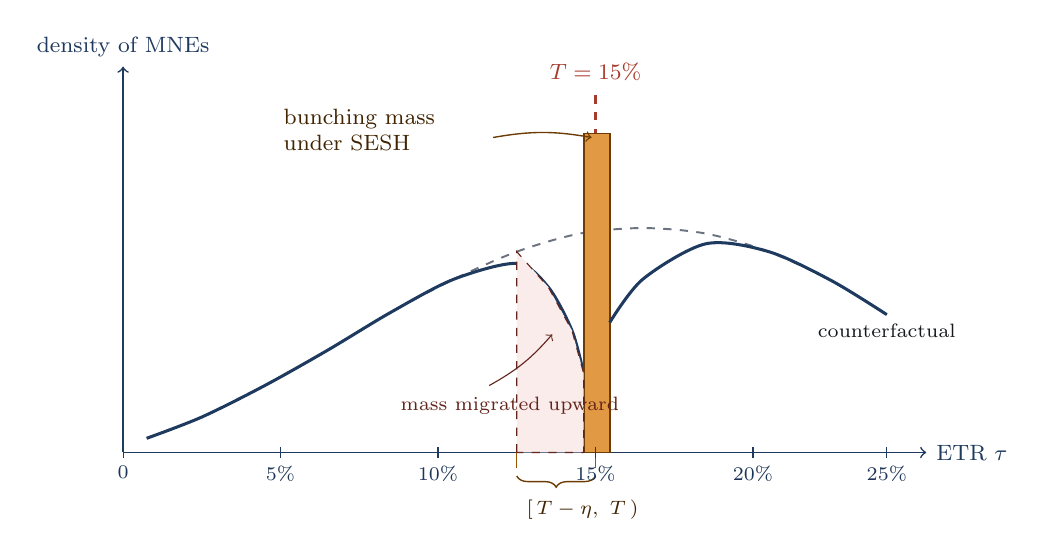
\begin{tikzpicture}[font=\small]
  % Coordinate system
  \def\xmax{10.0}
  \def\ymax{4.6}

  % Axes
  \draw[->, thesisNavy, line width=0.6pt] (0,0) -- (\xmax+0.2, 0) node[right, font=\footnotesize] {ETR $\tau$};
  \draw[->, thesisNavy, line width=0.6pt] (0,0) -- (0, \ymax+0.3) node[above, font=\footnotesize] {density of MNEs};

  % x-tick: 15%
  \def\Tx{6.0}
  \draw[thesisRed!85!black, dashed, line width=0.9pt] (\Tx,0) -- (\Tx,\ymax);
  \node[font=\footnotesize, thesisRed!85!black, anchor=south] at (\Tx,\ymax) {$T = 15\%$};

  % Counterfactual smooth density (no policy)
  % Bell-ish, peaked around tau=18
  \draw[thesisGrey, dashed, line width=0.7pt]
    plot[smooth] coordinates {
      (0.3,0.18) (1.0,0.45) (1.8,0.85) (2.6,1.30) (3.4,1.78)
      (4.2,2.20) (5.0,2.55) (5.8,2.78) (6.6,2.85) (7.4,2.78)
      (8.2,2.55) (9.0,2.18) (9.7,1.75)};
  \node[font=\scriptsize, thesisGrey!20!black, anchor=west] at (8.7, 1.55) {counterfactual};

  % Post-policy density: dip just before T, spike at T
  \draw[thesisNavy, line width=1.1pt]
    plot[smooth] coordinates {
      (0.3,0.18) (1.0,0.45) (1.8,0.85) (2.6,1.30) (3.4,1.78)
      (4.2,2.20) (5.0,2.40) (5.4,2.10) (5.7,1.55) (5.85,1.0)};

  % Spike (bunching mass) at 15%
  \fill[thesisOrange!75, draw=thesisOrange!50!black, line width=0.6pt]
    (5.85,0) rectangle (6.18, 4.05);
  \draw[thesisOrange!50!black, ->, line width=0.5pt] (4.7, 4.0) to[bend left=10] (5.95, 4.0);
  \node[font=\footnotesize, thesisOrange!30!black, align=left] at (3.0, 4.1)
    {bunching mass\\under SESH};

  % Resume after T
  \draw[thesisNavy, line width=1.1pt]
    plot[smooth] coordinates {
      (6.18,1.65) (6.6,2.20) (7.4,2.65) (8.2,2.55) (9.0,2.18) (9.7,1.75)};

  % Bunching window [T-eta, T)
  \def\TminEta{5.0} % Left boundary aligned with dashed reference line
  \draw[thesisOrange!70!black, line width=0.5pt] (\TminEta,0.05) -- (\TminEta,-0.20);
  \draw[thesisOrange!70!black, line width=0.5pt] (\Tx,0.05) -- (\Tx,-0.20);
  \draw[decorate, decoration={brace, mirror, amplitude=4pt}, thesisOrange!50!black, line width=0.5pt]
    (\TminEta,-0.30) -- (\Tx,-0.30);
  \node[font=\scriptsize, thesisOrange!30!black, anchor=north west]
    at (\TminEta, -0.48) {$[\,T-\eta,\ T\,)$};

  % x ticks
  \foreach \xv/\lbl in {0/0, 2/{5\%}, 4/{10\%}, 6/{15\%}, 8/{20\%}, 9.7/{25\%}}{
    \draw[thesisNavy] (\xv, 0.07) -- (\xv, -0.07);
    \node[below, font=\scriptsize, thesisNavy!90!black] at (\xv, -0.05) {\lbl};
  }

  % Mass missing region (hatched)
  \fill[thesisRed!10, draw=thesisRed!50!black, dashed, line width=0.4pt]
    (5.0, 0) -- (5.0, 2.55) -- (5.4,2.10) -- (5.7,1.55) -- (5.85,1.0) -- (5.85,0) -- cycle;
  \node[font=\scriptsize, thesisRed!50!black, anchor=west] at (3.4, 0.6) {mass migrated upward};
  \draw[thesisRed!50!black, ->, line width=0.4pt] (4.65, 0.85) to[bend right=10] (5.45, 1.5);
\end{tikzpicture}
\caption[Bunching at the 15\% threshold under the Simplified ETR Safe Harbour.]{Density of jurisdiction-level ETRs before and after the introduction of the Simplified ETR Safe Harbour. The dashed grey curve represents the counterfactual density absent any policy response, the solid navy curve represents the post-policy density. MNEs whose pre-policy ETR lies in the band $[T-\eta,\ T)$ migrate upward, producing the orange spike at the 15\% threshold. This is the \emph{notch} response that the SESH creates: the cost of falling just below 15\% is disproportionate to the saving, since the alternative is the full GloBE computation. The revenue pipeline treats this band as an upper-bound behavioural sensitivity with no cross-border reallocation and a zero top-up liability filter.}
\label{fig:sesh_bunching}
\end{figure}

The pipeline incorporates this response through a liability filter $m_{j,t}^{\text{beh}}$. The reallocation share $\hat{\beta}_{j,t}$ remains a cross-border profit-relocation object; the safe-harbour notch is not relocation, but movement of the simplified ETR onto the favourable side of the threshold:
\begin{equation}\label{eq:regime}
m_{j,t}^{\text{beh},e,m} = \begin{cases}
0 & \text{if } \tau_{j,t}^{\text{low},e} \in [T - \eta,\; T), \\[2pt]
1-\hat{\beta}_{j,t}^{e,m} & \text{if } \tau_{j,t}^{\text{low},e} < T - \eta, \\[2pt]
1 & \text{otherwise.}
\end{cases}
\end{equation}
where $T = 0.15$ and the baseline bandwidth is $\eta = 0.02$. Inside the bunching band $[T-\eta, T)$, jurisdictions reach the safe harbour through covered-tax and income management alone; the top-up tax is set to zero and pre-tax profit stays in place. In the code this means $\hat{\beta}_{j,t}^{e,m}=0$ but $m_{j,t}^{\text{beh},e,m}=0$. Below the band, the gap cannot be closed through accounting adjustments and the semi-elasticity response of \eqref{eq:beta_aggregated} applies. The bandwidth $\eta$ is a sensitivity parameter: $\eta \in \{0.01, 0.03\}$ bracket conservative and expansive variants, with the $\eta = 0.02$ baseline anchored on the dispersion evidence of \citet{hugger2026} and on the plausible cumulative scope of documented GloBE accounting adjustments. The notation should therefore be read as an upper-bound counterfactual, not as a structural bunching estimate. The structural route for a later paper is to replace the binary band with an estimated response probability once post-SESH microdata can identify the excess mass at fifteen per cent and the residual mass left in the dominated region.\footnote{The current rule assumes that \emph{every} jurisdiction inside $[T-\eta,T)$ reaches the safe harbour, whereas in reality the bunching mass depends on the distribution of ETRs within the band and on the within-jurisdiction elasticity of the simplified ETR with respect to covered-tax choices. Later the counterfactual density from pre-reform public CbCR is estimated, but that object remains a placebo and exposure diagnostic until post-reform observations exist.}

\subsubsection{Redistribution of reallocated profit}\label{sec:reallocation}

When a firm stops shifting profit to a haven, that profit shows up somewhere else. The thesis therefore adopts the formulary reallocation of \citet{garcia-bernardo2024}:
\begin{equation}\label{eq:reallocation}
R_i = \tfrac{1}{4}\frac{N_i}{\sum_{k} N_k} + \tfrac{1}{4}\frac{W_i}{\sum_{k} W_k} + \tfrac{1}{2}\frac{\text{UPR}_i}{\sum_{k} \text{UPR}_k},
\end{equation}
with $N_i$ employment, $W_i$ payroll, and $\text{UPR}_i$ unrelated-party revenue of MNE activity in destination $i$. Summation is restricted to destinations with $\tau_{i,t} \geq T$ so that reallocated profit is not mechanically re-deposited in a second haven.

Redistribution does not itself generate EU revenue. An additional euro sent to a jurisdiction with $\tau_{i,t}\ge T$ enters its GloBE base above the floor and contributes zero to the top-up. EU revenue from the GMT is determined entirely by the low-taxed source, not by the high-tax destination. The step is therefore diagnostic: \eqref{eq:reallocation} verifies profit conservation across counterfactuals and checks whether the implied re-reporting pattern aligns with the distribution of real activity. The SBIE is evaluated on \emph{pre-response} payroll and tangible assets throughout, holding the substance shield fixed across counterfactual simulations. Allowing substance to move in the same period would conflate two conceptually distinct margins: the short-run profit-allocation response identified by the semi-elasticity, and the long-run real-activity response documented in \citet{bilicka2022} and \citet{suarezserrato2018} and discussed in Section \ref{sec:limitations}.

Additional uncertainty is quantified in Appendix \ref{sec:beta_uncertainty}, which separates coefficient uncertainty from scenario spread and explains why the factorial behavioural contrast should not be read as a confidence interval.

\subsection{Revenue allocation and the Side-by-Side Safe Harbour}\label{sec:sbs}\label{sec:jan2026}

By this point the thesis has computed how much top-up tax exists. It has not yet said who collects it. The allocation rule is the piece that turns an aggregate liability into a country-by-country revenue line, and it is also the piece that the January 2026 Side-by-Side Safe Harbour reshapes. Under the standard GloBE rule order, the source jurisdiction collects the top-up tax via a QDMTT. If no QDMTT is in place, the parent jurisdiction collects via the IIR. If the parent has not implemented the IIR either, third-country jurisdictions collect via the UTPR.

The January 2026 Side-by-Side (SbS) Safe Harbour disrupts this rule order \citep{oecd2026}. MNE groups headquartered in jurisdictions with a ``Qualified SbS Regime'' may elect a deemed top-up tax of zero under both the IIR and the UTPR for all their operations. The United States is currently the only jurisdiction with a qualified regime.\footnote{The SbS Safe Harbour requires both an eligible domestic tax regime \emph{and} an eligible worldwide tax regime. The US qualifies through its combination of the corporate income tax (domestic) and the GILTI regime (worldwide). See \citet{oecd2026}, Chapter 1, Section 4.} US-parented MNEs are therefore exempt from IIR and UTPR enforcement.

QDMTTs remain entirely unaffected by the SbS Safe Harbour. Jurisdictions that implement a QDMTT retain the right to tax US-owned affiliates operating within their borders, regardless of the SbS election. The SbS package therefore creates a sharp discontinuity: for US-parented MNEs, the IIR and UTPR channels are switched off, but the QDMTT channel remains operational. 


Let $L_{p,j,t}$ denote the post-behaviour, pre-allocation top-up liability from equation \eqref{eq:pipeline}. The implemented source-level waterfall assigns this liability to four mutually exclusive pools:
\begin{align}
L_{p,j,t}^{\text{Q}} &= \mathbb{1}_j^{\text{Q}} L_{p,j,t}, \label{eq:qdmtt_sbs} \\
L_{p,j,t}^{\text{I}} &= (1-\mathbb{1}_j^{\text{Q}})\mathbb{1}_p^{\text{IIR}}(1-\mathbb{1}_p^{\text{SbS}})L_{p,j,t}, \label{eq:iir_sbs} \\
L_{p,j,t}^{\text{U}} &= (1-\mathbb{1}_j^{\text{Q}})(1-\mathbb{1}_p^{\text{IIR}})(1-\mathbb{1}_p^{\text{SbS}})L_{p,j,t}, \label{eq:utpr_sbs} \\
L_{p,j,t}^{\text{S}} &= (1-\mathbb{1}_j^{\text{Q}})\mathbb{1}_p^{\text{SbS}}L_{p,j,t}. \label{eq:sbs_extinguish}
\end{align}
The first pool is collected by the source jurisdiction $j$ through a QDMTT. The second is collected by the parent jurisdiction $p$ through the IIR. The third is a UTPR pool. The fourth is not revenue: it is the liability extinguished by the SbS election after the source jurisdiction has declined, or lacks, a QDMTT. Under the universal regime $\mathbb{1}_p^{\text{SbS}}=0$ for all parents; under the SbS regime it equals one for qualified US-parented groups.

The UTPR pool is not assigned back to the source jurisdiction. It is allocated to implementing collector jurisdictions $s$ using parent-year substance weights built from the public CbCR employee and tangible-asset variables:
\begin{equation}\label{eq:utpr_weight}
\omega_{s,p,t}^{\text{U}}
=
\frac{
\mathbb{1}_s^{\text{UTPR}}
\left[
\tfrac{1}{2}\frac{N_{p,s,t}}{\sum_{h:\mathbb{1}_h^{\text{UTPR}}=1}N_{p,h,t}}
+
\tfrac{1}{2}\frac{A_{p,s,t}}{\sum_{h:\mathbb{1}_h^{\text{UTPR}}=1}A_{p,h,t}}
\right]
}{
\sum_{h:\mathbb{1}_h^{\text{UTPR}}=1}
\left[
\tfrac{1}{2}\frac{N_{p,h,t}}{\sum_{r:\mathbb{1}_r^{\text{UTPR}}=1}N_{p,r,t}}
+
\tfrac{1}{2}\frac{A_{p,h,t}}{\sum_{r:\mathbb{1}_r^{\text{UTPR}}=1}A_{p,r,t}}
\right]
}.
\end{equation}
If only the employee or asset denominator is available, the implemented weight uses the available share alone. If no parent-year collector activity is available, the code falls back to a global year-level UTPR weight. Collector revenue is therefore:
\begin{align}
R_{s,t}^{\text{QDMTT}} &= \sum_p \sum_j \mathbb{1}\{s=j\}L_{p,j,t}^{\text{Q}}, \\
R_{s,t}^{\text{IIR}} &= \sum_p \sum_j \mathbb{1}\{s=p\}L_{p,j,t}^{\text{I}}, \\
R_{s,t}^{\text{UTPR}} &= \sum_p \sum_j \omega_{s,p,t}^{\text{U}}L_{p,j,t}^{\text{U}}.
\end{align}
Equation \eqref{eq:sbs_extinguish} formalises the core SbS consequence: US-parented residual IIR and UTPR liability is mechanically extinguished unless a QDMTT collects it first.

\begin{figure}[H]
\centering
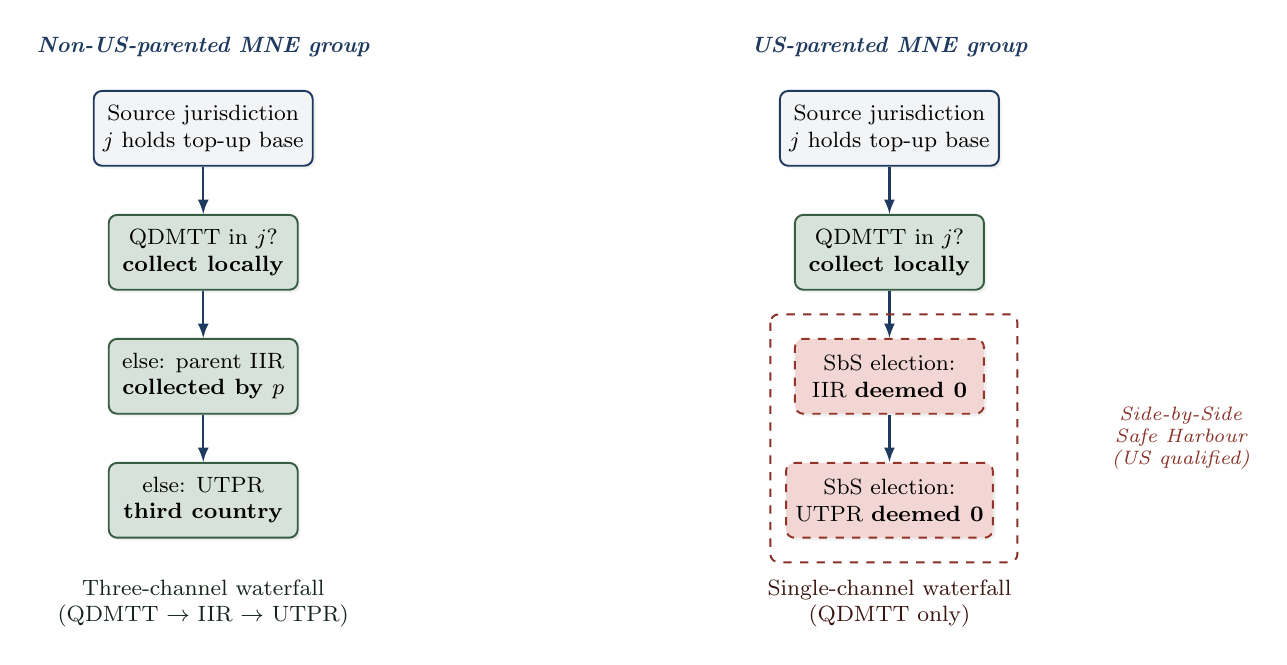
\begin{tikzpicture}[font=\small, node distance=0.6cm,
    rule/.style={draw=thesisNavy, line width=0.7pt, rounded corners=3pt,
                 fill=thesisLight, minimum width=2.4cm, minimum height=0.95cm,
                 align=center, font=\footnotesize,
                 drop shadow={shadow xshift=1pt, shadow yshift=-1pt, opacity=0.12}},
    on/.style={fill=thesisGreen!22, draw=thesisGreen!75!black},
    off/.style={fill=thesisRed!22, draw=thesisRed!75!black, dashed}]

  % Header rows
  \node[font=\footnotesize\itshape, thesisNavy] (h1) {\textbf{Non-US-parented MNE group}};
  \node[font=\footnotesize\itshape, thesisNavy, right=4.6cm of h1] (h2) {\textbf{US-parented MNE group}};

  %  Left column 
  \node[rule, below=0.3cm of h1] (sl) {Source jurisdiction\\$j$ holds top-up base};
  \node[rule, on, below=of sl] (q1) {QDMTT in $j$?\\\textbf{collect locally}};
  \node[rule, on, below=of q1] (i1) {else: parent IIR\\\textbf{collected by $p$}};
  \node[rule, on, below=of i1] (u1) {else: UTPR\\\textbf{third country}};

  %  Right column 
  \node[rule, below=0.3cm of h2] (sr) {Source jurisdiction\\$j$ holds top-up base};
  \node[rule, on, below=of sr] (q2) {QDMTT in $j$?\\\textbf{collect locally}};
  \node[rule, off, below=of q2] (i2) {SbS election:\\IIR \textbf{deemed 0}};
  \node[rule, off, below=of i2] (u2) {SbS election:\\UTPR \textbf{deemed 0}};

  % Arrows
  \foreach \a/\b in {sl/q1, q1/i1, i1/u1} \draw[thesis arrow] (\a) -- (\b);
  \foreach \a/\b in {sr/q2, q2/i2, i2/u2} \draw[thesis arrow] (\a) -- (\b);

  % SbS exemption banner spanning right column
  \draw[thesisRed!70!black, line width=0.7pt, rounded corners=3pt, dashed]
    ([xshift=-0.3cm, yshift=0.3cm]i2.north west) rectangle ([xshift=0.3cm, yshift=-0.3cm]u2.south east);
  \node[font=\scriptsize\itshape, thesisRed!70!black, align=center]
    at ($(i2)!0.5!(u2) + (3.7, 0)$) {Side-by-Side\\Safe Harbour\\(US qualified)};

  % Outcome at the bottom of each column
  \node[below=0.4cm of u1, font=\footnotesize, thesisGreen!30!black, align=center]
    {Three-channel waterfall\\(QDMTT $\to$ IIR $\to$ UTPR)};
  \node[below=0.4cm of u2, font=\footnotesize, thesisRed!30!black, align=center]
    {Single-channel waterfall\\(QDMTT only)};

\end{tikzpicture}
\caption[Allocation rule under the Side-by-Side Safe Harbour.]{Collection waterfall under the original GloBE rule order versus the January 2026 Side-by-Side Safe Harbour. For non-US-parented MNE groups, the QDMTT/IIR/UTPR cascade is unaffected. For US-parented groups, an SbS election sets both IIR and UTPR top-up to zero, leaving QDMTTs as the only operative collection channel. EU Member States that have not implemented a QDMTT therefore lose the residual top-up tax claim against US-owned affiliates, formalised in equation \eqref{eq:sbs_extinguish}.}
\label{fig:sbs_waterfall}
\end{figure}

\subsection{Counterfactual revenue equation}\label{sec:pipeline}

The measured data objects and the behavioural counterfactual combine into one compact equation. Read it from left to right: a euro of corrected profit is multiplied by the share that is low-taxed and the average top-up rate on that slice, then by the fraction not shielded by the SBIE, then by the behavioural liability filter, and finally routed to the country that has the right to collect it.\footnote{The revenue equation decomposition is original to this thesis. The individual components draw on \citet{hugger2026} for the low-taxed-profit measurement, \citet{schjelderup2024} and \citet{devereux2023} for the substance filter, and the panel-estimated semi-elasticities (Section \ref{sec:estimation}) for the behavioural counterfactual. No prior study combines these into a single multiplicative framework that makes the sources of revenue uncertainty simultaneously visible and exactly decomposable.} For each bilateral parent--affiliate cell, the pre-allocation top-up liability is:
\begin{equation}\label{eq:pipeline}
L_{p,j,t} = \underbrace{\ell_{p,j,t} \cdot \bar{\delta}_{j,t}^{\text{top}}}_{\text{ETR measurement}} \times \underbrace{\left(1 - \bar{\phi}_{p,j,t}\right)}_{\text{SBIE measurement}} \times \underbrace{m_{j,t}^{\text{beh}}}_{\text{behavioural counterfactual}}
\end{equation}
where $\ell_{p,j,t} = s_{j,t}^{<T} \cdot \pi_{p,j,t}^{*}$ is low-taxed profit (Section \ref{sec:etr_measurement}), $\bar{\delta}_{j,t}^{\text{top}}$ is the average top-up rate on that low-taxed portion, $\bar{\phi}_{p,j,t}$ is the SBIE shield (Section \ref{sec:SBIE}), and $m_{j,t}^{\text{beh}}$ is the behavioural liability filter defined in \eqref{eq:regime}, with ETR-measurement and semi-elasticity-model superscripts suppressed. The allocation rule then distributes the liability:
\begin{equation}\label{eq:allocation}
R_{s,t}^{(r)} = \sum_p \sum_j a_{s,p,j,t}^{(r)} \cdot L_{p,j,t}
\end{equation}
where $a_{s,p,j,t}^{(r)}$ is the regime-specific allocation weight implied by the QDMTT/IIR/UTPR rule order under policy regime $r$ (Section \ref{sec:sbs}). For UTPR liabilities, $a_{s,p,j,t}^{(r)}$ is the parent-year substance weight in \eqref{eq:utpr_weight}, or the global year-level fallback where no parent-year collector key is available.

Revenue uncertainty compounds across the measured objects and the behavioural counterfactual. A positive ETR-measurement $\times$ SBIE interaction indicates that the distributional approach reveals low-taxed profit concentrated in capital-intensive sectors with high $\phi$, so the expanded base is partially offset by stronger SBIE shielding. The equation identifies which data improvements would most reduce uncertainty: if the ETR measurement dominates variation, within-jurisdiction ETR data are the priority; if the SBIE measurement dominates, better CbCR coverage of tangible assets and payroll matters more.

\subsection{Counterfactual decomposition}\label{sec:decomposition}

Revenue estimates of the GMT in the existing literature are scattered because authors make different modelling choices. The thesis runs the revenue pipeline under every combination of five contested assumptions, observes the resulting revenue number, and attributes the spread to each assumption and to every interaction between them. The purpose is econometric rather than cosmetic. The decomposition asks whether disagreement across revenue estimates comes mainly from measured endowments, especially the volume and composition of low-taxed profit, or from coefficients and rules applied to those endowments, especially behavioural semi-elasticities and legal collection rights. In that sense it parallels the Oaxaca--Blinder split between characteristics and returns \citep{oaxaca1973,blinder1973}. Because the design contains higher-order interactions, it also reports a Shapley-style attribution that allocates each interaction equally across the factors that create it.

\subsubsection{Factor definitions}\label{sec:factors}

Five binary factors drive the variation in GMT revenue estimates. Table \ref{tab:factors} defines each factor and its two levels.

\begin{table}[H]
\centering
\caption{Decomposition factors}
\label{tab:factors}
\small
\begin{tabular}{@{}clp{3.5cm}p{3.5cm}@{}}
\toprule
Factor & Name & Baseline ($x_i = 0$) & Alternative ($x_i = 1$) \\
\midrule
1 & ETR measurement & Jurisdiction-average & Within-jurisdiction percentile approximation (Hugger-style) \\
2 & Substance specification & Aggregate SBIE (preferred public-CbCR estimate) & EU host-country sectoral bridge with SBTI-capacity overlay ($\kappa$) \\
3 & SBIE carve-out rates & Initial (10\%/8\%) & Long-run (5\%/5\%) \\
4 & SbS carve-out & Universal IIR/UTPR & SbS Safe Harbour (US exempt from IIR/UTPR) \\
5 & Behavioural response & None (mechanical) & BIC-preferred panel semi-elasticity + SESH liability filter \\
\bottomrule
\end{tabular}
\end{table}

Each factor maps to one component of the measured or counterfactual revenue equation. Factor 1 switches $s_j^{<T}$ between binary and continuous, so it is an endowment factor: it changes the measured quantity of low-taxed profit. Factor 2 changes $\bar{\phi}_{p,j,t}$ from the aggregate CbCR value to a sectoral host-country bridge with the SBTI-capacity overlay ($\kappa_{j,s,t}$ from equation \ref{eq:sbti_capacity}). This is also an endowment factor, because it changes the measured payroll and tangible-asset shield attached to the same profit base. The sectoral alternative is not the preferred point estimate: FATS is not restricted to Pillar Two in-scope groups, and it contains no ETR information. Its role is to show how sectoral composition would change the substance shield if public EU host-country sector shares are imposed on the aggregate CbCR base. Factor 3 moves from initial to long-run carve-out rates; it is a policy-parameter scenario rather than a statistical error. Factor 4 switches the allocation weight $a_{s,p,j,t}^{(r)}$ between universal and SbS regimes. Under the alternative, IIR and UTPR top-up variables are set to zero for qualified US-parented residual liabilities (equations \ref{eq:iir_sbs}--\ref{eq:sbs_extinguish}). QDMTTs remain fully operational in both scenarios. Factor 5 replaces the mechanical filter with $m_{j,t}^{\text{beh}}$: it applies $1-\hat{\beta}_{j,t}^{e,m}$ below the SESH bandwidth and a zero liability filter inside the bunching band $[T-\eta,T)$. This is the coefficient factor in the Oaxaca--Blinder analogy, because it changes the behavioural parameter applied to the measured tax base rather than the measured base itself.

Revenue is computed under all $2^5 = 32$ factor combinations.\footnote{The application of a full factorial design to GMT revenue estimation is original to this thesis. \citet{barake2022} and \citet{hugger2026} vary parameters one at a time; neither presents a design that makes all factor interactions simultaneously visible and exactly decomposable through orthogonal contrasts.} Let $\mathbf{x} = (x_1, \ldots, x_5) \in \{0, 1\}^5$ denote a configuration. The revenue under configuration $\mathbf{x}$ for EU Member State $j$ in year $t$ is $R_{j,t}(\mathbf{x})$.

The goal here is a statistical split of the revenue disagreement across assumptions. Each of the five modelling choices can be tested on its own, as can their combinations. A classical variance-decomposition identity, specialised to this balanced factorial design, gives an exact allocation of the total revenue spread to each single-factor effect and to every interaction between them. The algebra is the same orthogonal contrast machinery used in an ANOVA table, but the interpretation is structural: each contrast is attached to a named data, policy or behavioural mechanism in equation \eqref{eq:pipeline}. The $2^5$ factorial design permits an additive decomposition of the total sum of squares of revenue estimates into main effects, two-way interactions and higher-order interactions. For $K = 5$ factors the total variation of $R(\mathbf{x})$ across the 32 configurations is:
\begin{equation}\label{eq:anova}
\text{SS}_{\text{total}} = \sum_{i=1}^{5} \text{SS}_i + \sum_{i<k} \text{SS}_{ik} + \sum_{i<k<l} \text{SS}_{ikl} + \cdots + \text{SS}_{12345}
\end{equation}
where $\text{SS}_i$ is the sum of squares attributable to the main effect of factor $i$, $\text{SS}_{ik}$ is the sum of squares attributable to the two-way interaction between factors $i$ and $k$, and so forth. With five binary factors, the decomposition yields 5 main effects, 10 two-way interactions, 10 three-way interactions, 5 four-way interactions, and 1 five-way interaction, totalling $2^5 - 1 = 31$ orthogonal contrasts that exactly exhaust the total variation.

Each effect is computed from the orthogonal contrast in the balanced design. For a main effect of factor $i$:
\begin{equation}\label{eq:main_effect}
\text{SS}_i = \frac{n}{4} \left(\bar{R}_{x_i = 1} - \bar{R}_{x_i = 0}\right)^2
\end{equation}
where $\bar{R}_{x_i = 1}$ and $\bar{R}_{x_i = 0}$ are the mean revenues across all configurations where factor $i$ is at its high and low levels respectively, and $n = 32$ is the total number of configurations. For a two-way interaction:
\begin{equation}\label{eq:interaction_effect}
\text{SS}_{ik} = \frac{n}{16} \left(\bar{R}_{x_i = 1, x_k = 1} - \bar{R}_{x_i = 1, x_k = 0} - \bar{R}_{x_i = 0, x_k = 1} + \bar{R}_{x_i = 0, x_k = 0}\right)^2
\end{equation}
A non-zero two-way interaction $\text{SS}_{ik}$ indicates that the effect of factor $i$ on revenue depends on the level of factor $k$. For instance, a large $\text{SS}_{15}$ (ETR measurement $\times$ behavioural response) would indicate that the distributional ETR approach reveals low-taxed profit concentrated at very low pre-reform ETRs, where the nonlinear behavioural response is strongest, thereby amplifying the revenue difference between the two ETR approaches. A large $\text{SS}_{14}$ (ETR measurement $\times$ SbS regime) has a different economic meaning: it says that the low-taxed profit newly revealed by the distributional measurement is disproportionately attached to US-parented groups in jurisdictions where the SbS Safe Harbour extinguishes IIR and UTPR collection. The interaction is therefore a statement about the geography and ownership of the tax base. 

The share of explained variance attributable to each effect is $\eta_i^2 = \text{SS}_i / \text{SS}_{\text{total}}$. The first table reports the orthogonal contrasts directly. The second table reports a Shapley-style allocation in which each interaction share is divided equally across the factors that enter it. This second presentation answers the policy question, ``which mechanism ultimately accounts for the scenario spread once interactions are fairly attributed?'' The decomposition is performed at three levels: pooled across all 27 EU Member States and years, identifying which factors drive aggregate EU revenue variation, separately for each EU Member State (pooling across years), identifying country-specific dominant factors, and for selected EU Member States of policy interest (the Netherlands, Ireland, Luxembourg, Germany, France).

\subsubsection{Scenario spread versus estimation uncertainty}\label{sec:two_uncertainties}

The factorial design separates two conceptually distinct sources of uncertainty in GMT revenue estimates. \emph{Scenario spread} is the range of revenue estimates across the 32 modelling configurations for a given country--year cell, holding the semi-elasticity coefficients at their point estimates. This spread is driven by modelling assumptions that cannot be settled by the current public data alone: the choice between average and distributional ETR measurement, whether to use aggregate or sectoral SBIE, and whether the SbS regime applies. It is therefore primarily epistemic. \emph{Estimation uncertainty} is the confidence interval around the revenue estimate within a single scenario that would arise from resampling or otherwise propagating the Hines--Rice coefficient variance. It is aleatoric because it reflects statistical noise in the estimated behavioural coefficients.

For each EU Member State $j$ and year $t$, the ratio of scenario spread to estimation uncertainty is:
\begin{equation}\label{eq:spread_ratio}
\Lambda_{j,t} = \frac{\max_{\mathbf{x}} R_{j,t}(\mathbf{x}) - \min_{\mathbf{x}} R_{j,t}(\mathbf{x})}{q_{0.95}(R_{j,t}^{*}) - q_{0.05}(R_{j,t}^{*})}
\end{equation}
where $R_{j,t}^{*}$ denotes the preferred-scenario revenue estimate across coefficient-uncertainty draws once that propagation exercise is run. A ratio $\Lambda > 1$ indicates that the modelling assumptions matter more than the statistical precision of the semi-elasticity estimates. In that case, the debate about \emph{how} to estimate GMT revenue dominates the question of \emph{how precisely} the key behavioural parameter is known. This distinction is directly policy-relevant. If $\Lambda \gg 1$, reducing revenue uncertainty requires better data or institutional knowledge (such as within-jurisdiction ETR microdata), not more observations for the semi-elasticity regression. In the current results, the reported Stage 4.6 tables focus on scenario spread; Stage 1 measurement-error intervals are reported separately where generated, and coefficient bootstrap propagation should be treated as a next implementation step rather than as an already completed result.

\subsection{Hypotheses}\label{sec:hypotheses}

The methodology is now fully specified. Five predictions follow from it, one for each of the central claims the thesis wants to test. Each hypothesis states the a-priori expectation, the null hypothesis against which it is tested, and the test procedure. The five hypotheses map to the three subquestions: H1 addresses SQ1 (semi-elasticity estimation), H2 and H3 address SQ2 (factorial decomposition), and H4 and H5 address SQ3 (January 2026 provisions).

\textbf{H1: The profit-shifting semi-elasticity is nonlinear across the ETR distribution, rising sharply at low ETRs, and the logarithmic functional form captures this nonlinearity better than the linear or quadratic alternatives.}

$H_0$: The semi-elasticity of reported profits with respect to the ETR is constant across the tax rate distribution ($\beta_4 = 0$ in both the quadratic and logarithmic specifications), and the linear model fits the CbCR panel at least as well as the nonlinear alternatives.

\textit{A-priori expectation:} Profit shifting via intellectual property relocation and intra-group lending involves largely fixed set-up costs (legal structures, treaty planning, intercompany agreements). As the ETR approaches zero, these fixed costs become a smaller fraction of the tax saving, so the marginal MNE finds it profitable to shift at increasingly small tax differentials. This produces a convex cost function and a semi-elasticity that rises sharply at low ETRs. \citet{dowd2017} document this on US IRS data: the semi-elasticity at a 5\% statutory rate is 4.7, compared to 0.7 at 30\%. \citet{garcia-bernardo2024} confirm the pattern on a 2017 OECD CbCR cross-section, finding that the logarithmic specification (which allows unbounded semi-elasticity as $\tau \to 0$) dominates the quadratic (which imposes a turning point). The pre-specified expectation is that the logarithmic specification produces the lowest BIC, is preferred by the Vuong test, and yields a panel-estimated semi-elasticity at $\tau = 0.05$ exceeding the meta-regression consensus of 0.8 \citep{heckemeyer2017} by a factor of at least three. The panel structure adds within-pair variation that the cross-section lacks, reducing omitted-variable bias from time-invariant bilateral confounders.

\textbf{H2: The ETR measurement method accounts for the largest share of explained variance in the factorial decomposition of GMT revenue estimates.}

$H_0$: The five main effects contribute equally to the total variance of revenue estimates across the 32 factorial configurations ($\eta_1^2 = \eta_k^2$ for all $k$).

\textit{A-priori expectation:} The ETR measurement factor (jurisdiction-average vs.\ distributional) operates at the base level of the revenue pipeline: it determines $s_{j,t}^{<T}$, the share of profit classified as low-taxed, on which all subsequent components act multiplicatively. \citet{hugger2026} show that 53.2\% of global low-taxed profit lies in jurisdictions with average ETRs above 15\%, implying that the distributional approach approximately doubles the measured GMT base. This base-level doubling is expected to dominate the multiplicative adjustments from the other four factors. The SBIE shields 57\% of GloBE income on average \citep{devereux2023}, so switching from aggregate to sectoral SBIE changes revenue by the difference in $\phi$ across specifications. This is a second-order effect relative to doubling the base. The behavioural response under the linear benchmark implies an 8\% profit reduction at $\tau = 5\%$; even the nonlinear logarithmic response, applied to a fixed base, generates less variation than switching between a base of $X$ and $2X$. A potential rejection arises if the panel-estimated nonlinear semi-elasticities produce behavioural adjustments large enough to rival the base doubling, which would occur if the EU low-tax base is concentrated at near-zero pre-reform ETRs where the logarithmic semi-elasticity is steepest.

\textbf{H3: Factor interactions account for an economically significant share of total revenue variation, implying that one-at-a-time sensitivity analysis understates the true uncertainty range.}

$H_0$: All interaction effects are zero; the total variation is fully explained by the five main effects ($\text{SS}_{\text{interactions}} = 0$).

\textit{A-priori expectation:} Published GMT revenue estimates vary parameters individually: \citet{barake2022} report estimates with and without behavioural responses; \citet{hugger2026} compare average and distributional ETR approaches; \citet{boukal2026} decompose by collection channel. None examines joint variation. The revenue pipeline (equation \ref{eq:pipeline}) is multiplicative, which makes non-zero interactions likely. The behavioural response reduces a \emph{percentage} of the base, so its absolute effect depends on whether the base was measured with the average or distributional approach (the Factor 1 $\times$ Factor 5 interaction). Similarly, the SBIE filter interacts with ETR measurement if the newly revealed low-taxed profit (from the distributional approach) is concentrated in holding/IP entities with low substance, differing from the composition of profit already classified as low-taxed under the average approach. The SbS carve-out (Factor 4) interacts with ETR measurement (Factor 1) if the distributional approach reveals substantial US-parented low-taxed profit in non-QDMTT jurisdictions. The pre-specified expectation is that the total interaction share exceeds 10\%.

\textbf{H4: The SbS Safe Harbour reduces aggregate EU GMT revenue collected through the IIR and UTPR channels, with the revenue loss concentrated in Member States that have not implemented a QDMTT.}

$H_0$: The SbS Safe Harbour has no effect on aggregate EU GMT revenue ($\bar{R}^{\text{SbS}} = \bar{R}^{\text{universal}}$), and the revenue change does not vary with QDMTT implementation status.

\textit{A-priori expectation:} The SbS mechanically eliminates residual IIR and UTPR collection on qualified US-parented MNE groups after any QDMTT has collected first (equations \ref{eq:qdmtt_sbs}--\ref{eq:sbs_extinguish}). QDMTTs remain fully operational. The net effect on a Member State's revenue therefore depends on two quantities: the share of its low-taxed profit attributable to US-parented MNEs, and whether it has implemented a QDMTT. Member States with a QDMTT retain the right to tax US-owned affiliates domestically. Those without one lose the residual IIR or UTPR channel. US-parented MNEs account for approximately 30--40\% of global CbCR profits; the Dutch government projected a \EUR120 million annual reduction from the SbS package \citep{1028}. The pre-specified expectation is that aggregate EU revenue declines significantly, with the decline concentrated in Member States without a QDMTT.

\textbf{H5: The SBTI Safe Harbour reduces the effective tax floor heterogeneously across EU sectors, with the reduction largest in capital-intensive sectors.}

$H_0$: The SBTI-induced reduction in the effective tax floor is uniform across sectors ($\partial \Delta\tau^{\text{floor}} / \partial (A/\pi) = 0$).

\textit{A-priori expectation:} The SBTI allows MNEs to treat qualifying tax incentives as additions to covered taxes, bounded by a Substance Cap tied to payroll and tangible assets (equation \ref{eq:substance_cap}). Capital-intensive sectors benefit doubly: larger SBIE carve-outs \emph{and} higher Substance Caps. \citet{schjelderup2024} predict that the SBIE functions as a \emph{de facto} production subsidy favouring capital-intensive industries; the SBTI amplifies this by adding a second substance-linked benefit. Asset-light sectors (financial services, IP licensing) have Substance Caps approaching zero and therefore cannot utilise the SBTI. \citet{devereux2023} find SBIE-to-profit ratios ranging from below 30\% (financial services) to above 70\% (manufacturing), confirming the sectoral gradient. The countervailing force is that capital-intensive sectors may already face pre-reform ETRs above 15\%, reducing the set of entities for which the SBTI matters. The pre-specified expectation is that the capital-intensity effect dominates, producing a negative coefficient: higher $A/\pi$ is associated with a larger reduction (more negative $\Delta\tau^{\text{floor}}$).

\newpage

\section{Results}\label{sec:results}\label{sec:se_results}

This section reports the empirical results of the five-stage revenue pipeline and the factorial decomposition developed in the Data section \ref{sec:data} and Methodology \ref{sec:methodology}. Two findings define the answer to the research question. First, the choice between jurisdiction-average and within-jurisdiction distributional ETR measurement accounts for 62.2\% of pooled scenario variance in legally allocated EU GMT revenue, confirming that the heterogeneity documented by \citet{hugger2026} is the single largest driver of revenue disagreement. Second, the January 2026 Side-by-Side Safe Harbour accounts for a further 25.4\%, because it extinguishes residual IIR and UTPR collection on US-parented groups in the absence of a QDMTT. Together, these two factors explain 87.6\% of the revenue spread before any interaction term is allocated.

The econometric evidence qualifies the ex-ante expectations in two directions. The 2017--2022 CbCR panel yields a statistically significant linear semi-elasticity of 1.51 (two-way clustered $p = 1.6 \times 10^{-6}$), which exceeds the meta-regression consensus of approximately 0.8 \citep{heckemeyer2017} by a factor of 1.9. The estimate is, however, far below the steep low-rate nonlinearities reported by \citet{dowd2017} on US administrative data, where the semi-elasticity at a 5\% rate reaches 4.7. The BIC selects the linear specification over the logarithmic ($\Delta$BIC = 5.26) and quadratic ($\Delta$BIC = 7.56) alternatives, so the pre-specified expectation that the logarithmic form would dominate (H1) is only partly supported. The behavioural response contributes 3.4\% of pooled variance, and all interaction terms combined contribute 5.3\%, below the 10\% threshold set for H3. In the preferred-core scenario, cumulative EU revenue over 2017--2022 falls from US\$531.6 billion under universal IIR/UTPR collection to US\$362.1 billion under SbS treatment, a reduction of US\$169.5 billion driven entirely by the legal reallocation channel.

The section is organised as follows. Section \ref{sec:results_stage1} reports the measured low-taxed profit base under both ETR approaches. Section \ref{sec:results_stage2} applies the substance exclusion and quantifies the SBTI-capacity gradient across EU sectors. Section \ref{sec:results_stage3} presents the panel semi-elasticity estimates and the IV diagnostics. Section \ref{sec:results_factorial} reports the factorial decomposition of legally allocated revenue. Section \ref{sec:results_sbs} examines country-level heterogeneity under the SbS regime. Section \ref{sec:results_hypotheses} summarises the hypothesis tests.

\subsection{Measured low-taxed profit}\label{sec:results_stage1}

The first empirical step measures the low-taxed profit base before substance exclusions, safe-harbour allocation and behavioural responses are applied. For each parent--affiliate--year cell, Stage 1 computes
\begin{equation}\label{eq:results_stage1_liability}
L_{p,j,t}^{(1),m}
= \pi_{p,j,t}^{*}\, s_{p,j,t}^{<T,m}\, \bar{g}_{p,j,t}^{m},
\end{equation}
where $\pi^{*}$ is corrected positive profit, $T=0.15$ is the GMT threshold, $s^{<T,m}$ is the profit share below the threshold under measurement branch $m$, and $\bar{g}^{m}$ is the profit-weighted average top-up gap on the relevant low-taxed profit mass. The superscript $m$ indexes the ETR measurement branch: under the average branch, $s^{<T,m}$ is a jurisdiction-level binary indicator based on the aggregate CbCR ETR; under the distributional branch, it is the fitted or directly observed within-jurisdiction mass below 15\%. This binary distinction is the core of Factor 1 in the factorial design and captures the measurement problem emphasised by \citet{hugger2026}: a jurisdiction can have an aggregate ETR above 15\% while still containing a substantial mass of subsidiary-level profit taxed below that threshold.

\input{generated/results_tables/stage1_rates.tex}

Table \ref{tab:stage1_rates_updated} reports the economic effect of the ETR measurement choice. In the EU27, the average rule classifies a larger share of profit as low-taxed than the distributional rule in every year, but it attaches a much smaller top-up gap to that profit. In 2022, for example, the average rule records 53.5\% low-taxed profit and a 1.8\% liability rate, while the distributional rule records 43.2\% low-taxed profit and a 3.6\% liability rate. The distributional estimate therefore doubles the 2022 EU liability rate even though it assigns a smaller share of total profit to the low-taxed slice.

The mechanism behind this reversal is as follows. Jurisdiction averages classify entire country cells as either entirely above or entirely below the threshold. When the aggregate ETR is below 15\%, this produces a high low-taxed share, but the cells that are classified as low-taxed sit close to the threshold, generating a small top-up gap. The distributional approach isolates the subsidiary-level profit mass that is genuinely below 15\% and attaches to that mass a deeper gap to the threshold. This is the empirical counterpart of the theoretical prediction in \citet{hugger2026}, who show that 53.2\% of all profit taxed below 15\% is located in jurisdictions whose jurisdiction-average ETR exceeds 15\%. The distributional approach raises the EU27 liability rate relative to the average rule in every year from 2017 to 2022. The pattern is more volatile globally, where the average rule's low-taxed share fluctuates from 30.8\% (2022) to 59.6\% (2018), driven by the changing CbCR reporting sample.

\input{generated/results_tables/stage1_bspi_validation.tex}

Table \ref{tab:stage1_bspi_updated} identifies where the early-year backcast is fragile. Lithuania, Croatia and Greece have total-variation distances of 0.66, 0.56 and 0.42 between the 2019--2020 anchor and the 2021--2022 validation period, and are therefore flagged as unstable. The Netherlands, Luxembourg and Ireland have much lower distances of 0.12, 0.11 and 0.06 respectively. The backcast is consequently strongest for the core conduit and investment-hub jurisdictions that matter most for GMT revenue, and less reliable for smaller EU jurisdictions whose observed low-taxed shares changed sharply after 2020. The three flagged jurisdictions are small-profit cells: their combined share of EU low-taxed profit is below 2\%, so the fragility does not materially affect the aggregate revenue estimates. This evidence supports using the BSPI transport as a necessary bridge for maintaining the pre-2019 factorial structure, not as independent evidence about true pre-2019 subsidiary-level tax distributions.

\input{generated/results_tables/stage1_measurement_error_interval.tex}

Table \ref{tab:stage1_measurement_error_interval} translates the Table I versus Table IV validation residuals into a Stage 1 measurement-error interval for the preferred ETR branch. The exercise holds the preferred ETR measurement, aggregate SBIE and initial-rate scenario fixed, then varies the legal regime and behavioural filter. It is therefore not a second scenario decomposition. It is a direct estimate of how much the imperfect ETR measurement branch alone can move the headline revenue number.

Appendix Section \ref{app:results_stage1} reports the Stage 1 diagnostics that are too granular for the main line of the argument. Appendix Tables \ref{tab:app_stage1_bspi_tv} and \ref{tab:app_stage1_conditioning} document the BSPI validation distribution and the percentile-conditioning filters. Appendix Table \ref{tab:app_stage1_crossval} reports the Table I versus Table IV cross-validation used to discipline the constrained-Beta fallback.

\subsection{Substance exclusion and SBTI capacity}\label{sec:results_stage2}

The second empirical step applies the substance filters that convert the statutory 15\% floor into a lower effective tax floor. The SBIE shields a payroll-and-asset amount from the top-up base, so Stage 2 replaces $L^{(1)}$ by
\begin{equation}\label{eq:results_stage2_liability}
L_{p,j,t}^{(2),m,r}
= L_{p,j,t}^{(1),m}\,(1-\phi_{p,j,t}^{r}),
\end{equation}
where $\phi^{r}$ is the SBIE-to-low-taxed-profit ratio under rate schedule $r$. This is the empirical counterpart of the mechanism discussed by \citet{devereux2023} and \citet{schjelderup2024}: a minimum tax with a substance carve-out raises the tax price of pure profit shifting while preserving a lower effective floor for profits backed by payroll and tangible assets.

\input{generated/results_tables/stage2_aggregate.tex}

Table \ref{tab:stage2_aggregate_updated} quantifies the aggregate shield. Under the EU27 distributional measurement branch, the Stage 1 liability rate is 5.07\%. The initial SBIE rates reduce it to 4.63\%, a decline of 0.44 percentage points, while the long-run 5\%/5\% endpoint raises it back to 4.80\%, recovering roughly half of the initial shield. The same pattern holds globally: the distributional liability rate falls from 4.23\% to 3.81\% under initial rates and to 3.97\% under long-run rates. Two implications follow. First, the SBIE matters, but it moves the liability rate by less than the ETR measurement branch does: the average-to-distributional switch raises the liability rate by 1.8 percentage points, while the SBIE at its most generous reduces it by 0.44 percentage points. Second, the transition schedule compresses the substance shield over time, meaning that GMT revenue will gradually rise as carve-out rates converge to the long-run endpoint. This ranking anticipates the factorial decomposition in Section \ref{sec:results_factorial}.

\input{generated/results_tables/stage2_sectoral_sbti.tex}

Table \ref{tab:stage2_sectoral_sbti} adds the Substance-Based Tax Incentive (SBTI) Safe Harbour capacity to the sectoral matrix. The EU27 profit-weighted effective floor falls from 14.2\% before SBTI to 11.9\% after SBTI, a reduction of 2.3 percentage points. The decline is materially larger in Germany and France, at 3.1 and 3.5 percentage points respectively, than in the Netherlands, Ireland and Luxembourg, where it is at or below 1.0 percentage point. This cross-country gradient reflects the sectoral composition of foreign-controlled activity: Germany and France host more manufacturing and capital-intensive services, which generate larger payroll and tangible-asset bases and therefore higher SBTI Substance Caps under equation \eqref{eq:substance_cap}. This is the pattern predicted by \citet{schjelderup2024}: substance-linked relief is most valuable where the foreign-controlled sectoral structure is more capital-intensive. The table should be read as an upper-bound exposure estimate, because public CbCR does not observe actual SBTI-qualifying incentive claims, safe-harbour elections, or the decomposition of tax credits into qualifying and non-qualifying categories.

\input{generated/results_tables/stage2_h5_regression.tex}

Table \ref{tab:stage2_h5_regression} formalises the sectoral pattern with a country fixed-effect regression of the SBTI-induced effective floor reduction on sectoral capital intensity. The coefficient on tangible-asset intensity (tangible assets per employee) is negative in both the unweighted and profit-weighted specifications and statistically significant under clustered inference. The unweighted coefficient is $-0.00007$ ($p=0.023$), and the profit-weighted coefficient is $-0.00162$ ($p=0.002$). Higher tangible-asset intensity is therefore associated with a larger reduction in the effective tax floor once the SBTI overlay is applied. H5 is supported: the GMT's substance exclusions do create a systematically lower effective floor for capital-intensive sectors, confirming the theoretical prediction that the SBIE and SBTI together function as a production subsidy embedded in the minimum-tax architecture \citep{schjelderup2024}. 

Appendix Section \ref{app:results_stage2} reports the two implementation checks behind the substance layer. Appendix Table \ref{tab:app_stage2_payroll_fallback} documents the wage-source hierarchy used for payroll imputation, while Appendix Table \ref{tab:app_stage2_asset_sensitivity} checks whether the asset leg changes materially when the sectoral asset allocator is varied.


\subsection{Behavioural semi-elasticities}\label{sec:results_stage3}

The third empirical step estimates how much low-taxed profit is reallocated once firms respond to the higher tax floor. The behavioural model is a two-way fixed-effect Hines--Rice regression (equation \ref{eq:panel_linear}) in which the coefficient on the ETR determines the semi-elasticity of reported profit with respect to the tax rate. With $\tau$ expressed as a unit rate, the linear estimate $\hat{\beta}_{\tau}$ maps directly to the semi-elasticity $\hat{\varepsilon}=-\hat{\beta}_{\tau}$, meaning that a one percentage-point increase in the ETR is associated with a $|\hat{\beta}_{\tau}|$\% reduction in reported profit, conditional on pair and year fixed effects. The nonlinear specifications evaluate the corresponding derivative at specific ETRs, which determines how much of the low-taxed base the counterfactual raises to 15\%.

\input{generated/results_tables/stage3_model_comparison.tex}

Table \ref{tab:stage3_model_comparison} gives the model-selection result. All three specifications are estimated on the same 8{,}971 observations and 1{,}936 parent--affiliate pairs over six fiscal years (2017--2022). The linear model has the lowest BIC, with the logarithmic model second ($\Delta$BIC = 5.26) and the quadratic model third ($\Delta$BIC = 7.56). A $\Delta$BIC above 2 is conventionally interpreted as positive evidence against the higher-BIC model \citep{raftery1995}, and a $\Delta$BIC above 6 as strong evidence. The joint Wald test on all tax terms is highly significant in every specification, with two-way clustered $p$-values around $10^{-6}$. The panel therefore contains a robust tax-profit relationship, but the pre-specified expectation that the logarithmic form would dominate the linear alternative (H1) is not supported by the BIC criterion.

\input{generated/results_tables/stage3_regression_table.tex}

Table \ref{tab:stage3_regression_table} presents the coefficient estimates. In the preferred linear specification, the ETR coefficient is $-1.506$ with a two-way clustered standard error of 0.273 ($t = -5.52$). A one percentage-point increase in the ETR is therefore associated with a 1.51\% reduction in reported profit in the affiliate jurisdiction, conditional on parent--affiliate pair fixed effects, year fixed effects, log tangible assets, log payroll proxy, log GDP per capita and log population. The substance controls (tangible assets and payroll) are individually insignificant, reflecting the pair fixed effects' absorption of the cross-sectional variation that drives substance variables in pooled regressions. GDP per capita is highly significant ($0.675$, $p < 0.001$), consistent with the standard Hines--Rice finding that profits correlate with market size conditional on tax incentives.

The sign and magnitude of the semi-elasticity place the estimate squarely between two poles of the existing literature. The meta-regression consensus in \citet{heckemeyer2017} reports a semi-elasticity of approximately 0.8. The present estimate of 1.51 is 89\% larger, consistent with the observation that the 2017--2022 panel captures a period of heightened profit shifting activity documented by \citet{garcia-bernardo2022a}. However, it is far below the steep low-rate nonlinearities in \citet{dowd2017}, who report semi-elasticities reaching 4.7 at 5\% ETRs using US administrative data that can distinguish real from paper profits. The quadratic term ($0.439$, $p = 0.729$) and the logarithmic term ($-0.209$, $p = 0.600$) are individually insignificant once pair fixed effects are imposed. The nonlinear specifications add one parameter but virtually no explanatory power: within $R^2$ rises from 0.0340 to 0.0341 (quadratic) and 0.0344 (logarithmic).

\input{generated/results_tables/stage3_iv_diagnostics.tex}

Table \ref{tab:stage3_iv_diagnostics} addresses the main endogeneity concern: the CbCR ETR uses reported profit in its denominator, so current profit shifting can mechanically change the tax variable. Both tax-code instruments have statistically significant first stages. The OECD simulated fixed-project EATR first-stage coefficient is 0.239 ($F = 11.28$, clustered); the lagged statutory CIT first-stage coefficient is 0.256 ($F = 20.34$, clustered). The lagged CIT instrument passes the \citet{stock2005} weak-instrument threshold of $F > 10$ comfortably; the simulated EATR instrument sits at the boundary. The reduced forms and FE-2SLS estimates are, however, imprecise and statistically insignificant. The simulated EATR FE-2SLS coefficient is $-0.437$ ($p=0.813$), and the lagged statutory CIT FE-2SLS coefficient is $-1.157$ ($p=0.468$).

The IV diagnostics do not overturn the fixed-effect association, but they limit its causal interpretation. The instruments move CbCR ETRs in the expected direction, yet they do not deliver a precise reduced-form profit response in the public panel. Three factors explain this result. First, the 2017--2022 window contains limited policy-driven tax variation after absorbing pair fixed effects. Second, the CbCR aggregation compresses affiliate-level heterogeneity that drives much of the cross-sectional response in \citet{garcia-bernardo2024}. Third, the concentration of profit shifting in a small number of conduit jurisdictions (Ireland, Luxembourg, the Netherlands) means the effective IV sample is driven by a narrow base. The behavioural counterfactual should therefore be read as an internally consistent reduced-form scenario, not as a fully causal micro-elasticity. The additional robustness checks in Appendix Table \ref{tab:app_stage3_robustness} confirm that the linear coefficient is stable across the balanced panel, the non-stale wage subsample, and the COVID-excluded window.

\input{generated/results_tables/stage3_semielasticity.tex}

Table \ref{tab:stage3_semielasticity} translates the coefficients into the reallocation schedule used in the revenue simulation. The preferred linear model gives a constant semi-elasticity of 1.51, implying reallocation shares of 14.0\% at a 5\% ETR and 7.3\% at a 10\% ETR when the effective rate is raised to the 15\% floor. The reallocation share is computed from equation \eqref{eq:beta_aggregated} as $1 - G_{\text{lin}}(\tau)$, where $G_{\text{lin}}(\tau) = \exp[\hat{\beta}_3 (T - \tau)]$. The nonlinear specifications produce somewhat larger low-rate responses: the logarithmic semi-elasticity is 2.02 at 5\% (reallocation share 16.6\%), while the quadratic gives 1.72 at 5\% (reallocation share 15.5\%). The 5\% logarithmic estimate is, however, significant only at the 10\% level ($p=0.081$), and the 5\% quadratic only at the 5\% level ($p=0.034$). The behavioural response is therefore sizeable enough to reduce top-up revenue materially: an aggregate reduction of US\$52.2 billion over the cumulative EU base. But it is too moderate and too weakly nonlinear to dominate the measurement and legal-regime factors.

Appendix Section \ref{app:results_stage3} reports the full behavioural diagnostics. Appendix Tables \ref{tab:app_stage3_sample_summary}, \ref{tab:app_stage3_tax_coefficients}, \ref{tab:app_stage3_specification_tests}, \ref{tab:app_stage3_wald_tests}, \ref{tab:app_stage3_etr_tail_support}, \ref{tab:app_stage3_behaviour_by_year} and \ref{tab:app_stage3_behavioural_design} document the estimation sample, tax coefficients, non-nested tests, joint tests, lower-tail support, year-by-year behavioural filter and identification boundary.

\subsection{Allocation and factorial decomposition}\label{sec:results_factorial}

The fourth empirical step turns liability into country revenue and asks which modelling choices drive the scenario spread. The decomposition is run over the full 32-scenario matrix and pooled across EU27 country-years. The result is clear: uncertainty is dominated by measurement of the low-taxed base and by the legal allocation regime, while the behavioural coefficient is statistically visible but quantitatively secondary.

\input{generated/results_tables/stage4_6_anova.tex}

Table \ref{tab:stage4_6_anova_updated} reports the orthogonal factorial decomposition. ETR measurement explains 62.2\% of pooled variance. The SbS regime explains 25.4\%. Substance specification and behavioural response explain 3.7\% and 3.4\%, respectively, while the SBIE rate endpoint explains only 0.1\%. The largest interaction is ETR measurement $\times$ SbS regime at 2.8\%, followed by ETR measurement $\times$ substance specification at 1.6\%. All interactions together explain 5.3\%, below the 10\% threshold specified in H3. The multiplicative pipeline therefore generates interactions, but the main effects already explain the substantive ordering.

\input{generated/results_tables/stage4_6_shapley_factor_attribution.tex}

Table \ref{tab:stage4_6_shapley_attribution} reallocates the interaction shares equally across the factors that create them. This gives the cleanest economic interpretation of the scenario variance. ETR measurement accounts for 64.7\% of allocated variation after interactions are included. The SbS regime accounts for 26.9\%. Substance specification accounts for 4.5\%, behavioural response for 3.8\%, and the SBIE rate endpoint for 0.1\%. The Shapley-style table therefore confirms the same conclusion as the raw ANOVA: the core uncertainty is epistemic measurement uncertainty and institutional legal-regime uncertainty. Statistical uncertainty in the behavioural coefficient is important for the behavioural scenario, yet it is not the dominant reason why GMT revenue estimates differ.

\input{generated/results_tables/stage4_6_main_effects.tex}

Table \ref{tab:stage4_6_main_effects} translates the variance shares into revenue levels. Moving from jurisdiction-average to distributional ETR measurement raises cumulative EU revenue from US\$195.1 billion to US\$400.7 billion, a main effect of US\$205.6 billion. Moving from universal IIR/UTPR collection to the SbS regime lowers cumulative EU revenue from US\$356.5 billion to US\$239.2 billion, a main effect of US\$117.3 billion. The behavioural response lowers revenue by US\$47.1 billion, and the sectoral SBIE with SBTI overlay lowers revenue by US\$42.6 billion. The behavioural channel therefore matters economically, but it does not rescue H1's stronger claim that the lower-tail semi-elasticity would dominate the revenue answer.

The decomposition changes the interpretation of the thesis relative to the proposal. The proposal expected a sharp nonlinear behavioural response to become the central empirical finding. The realised evidence rejects that stronger version. The linear semi-elasticity is significant and larger than the meta-regression consensus, but the main source of policy uncertainty is the construction of the taxable base and the legal rule that decides who may collect it. That is a stronger policy result than another elasticity estimate, because it tells the reader where better data and clearer guidance would reduce fiscal uncertainty most.


\subsection{SbS allocation and country heterogeneity}\label{sec:results_sbs}

The SbS regime changes EU revenue through the collection channel, not through the existence of low-taxed profit. QDMTTs remain operational, so source jurisdictions that have implemented a QDMTT keep the domestic top-up on US-owned affiliates. The loss appears in residual IIR and UTPR collection, especially where US-parented low-taxed profit would otherwise have been routed through the UTPR.

\input{generated/results_tables/preferred_channel.tex}

Table \ref{tab:preferred_channel_updated} shows the preferred-core channel allocation. Under universal collection, cumulative EU revenue is US\$531.6 billion: US\$201.4 billion through QDMTTs, US\$93.0 billion through the IIR and US\$237.2 billion through the UTPR source proxy. Under SbS, QDMTT and IIR revenue remain unchanged in the preferred core, while UTPR revenue falls to US\$67.8 billion. The implied SbS loss is therefore US\$169.4 billion in the preferred-core mechanical scenario. This is why Factor 4 is the second-largest source of scenario variance.

Appendix Section \ref{app:results_stage45} reports the allocation diagnostics behind the channel totals. Appendix Table \ref{tab:app_stage45_summary} records the Stage 4.5 scenario totals, Appendix Table \ref{tab:app_stage45_sbs_source_exposure} identifies the US-parented exposure affected by SbS, and Appendix Table \ref{tab:app_stage45_h4_regression} reports the country-level H4 regression check.

COUNTRY DECOMPOSITION ADD STILL

\subsection{Hypothesis summary}\label{sec:results_hypotheses}

\input{generated/results_tables/hypothesis_summary.tex}

Table \ref{tab:hypothesis_result_summary} summarises the five hypothesis tests. 


\section{Discussion and conclusion}\label{sec:discussion}

\newpage
\printbibliography[heading=bibintoc]

\newpage
\appendix
\renewcommand{\thesection}{\Alph{section}}
\renewcommand{\theHsection}{appendix.\Alph{section}}
\renewcommand{\theHsubsection}{appendix.\Alph{section}.\arabic{subsection}}
\renewcommand{\theHsubsubsection}{appendix.\Alph{section}.\arabic{subsection}.\arabic{subsubsection}}
\renewcommand{\thetable}{\Alph{section}.\arabic{table}}
\renewcommand{\thefigure}{\Alph{section}.\arabic{figure}}
\renewcommand{\theequation}{\Alph{section}.\arabic{equation}}
\renewcommand{\theHtable}{appendix.\Alph{section}.\arabic{table}}
\renewcommand{\theHfigure}{appendix.\Alph{section}.\arabic{figure}}
\renewcommand{\theHequation}{appendix.\Alph{section}.\arabic{equation}}
\setcounter{table}{0}
\setcounter{figure}{0}
\setcounter{equation}{0}

\section{Data appendix}\label{app:data}

\subsection{Unit of observation}\label{app:unit_obs}

The baseline unit of observation is a parent--affiliate--year cell $(p,j,t)$, where $p$ is the ultimate parent jurisdiction, $j$ is the affiliate jurisdiction, and $t$ is the fiscal year. ETR percentiles are pooled to affiliate-year cells before fitting the within-jurisdiction distribution; FATS shares are country-sector-year objects; implementation variables are jurisdiction-year or parent-year indicators. Table \ref{tab:data_sources_units} records these units explicitly, so that subsequent transformations do not silently mix levels of aggregation.

\begin{table}[H]
\centering
\caption{Data sources, original units, and measurement role}
\label{tab:data_sources_units}
\footnotesize
\begin{tabularx}{\textwidth}{@{}L{2.8cm}L{3.2cm}L{3.2cm}X@{}}
\toprule
Source & Original unit of observation & Main raw variables & Measurement role \\
\midrule
OECD CbCR Table I & Parent jurisdiction $\times$ affiliate jurisdiction $\times$ fiscal year $\times$ profit panel & \code{PROFIT}, \code{PROFIT\_ADJ}, \code{TAX\_ACCRUED}, \code{ASSETS}, \code{EMPLOYEES}, ETR percentiles, business-activity counts & Base bilateral panel, corrected profit, jurisdiction-average ETR, Table I constrained-Beta fit, aggregate SBIE inputs \\
OECD CbCR Table IV & Parent jurisdiction $\times$ affiliate jurisdiction $\times$ fiscal year $\times$ subsidiary-level ETR bracket & Profit, tax, assets, employees and activity counts by ETR bracket, especially \code{RATE\_0-15} & Direct observation of the low-taxed profit bracket and cross-validation of the Table I constrained-Beta fit \\
Eurostat inward FATS & Reporting country $\times$ NACE sector $\times$ controlling country $\times$ year & Employment, turnover, personnel costs, investment and value added & EU host-country sectoral exposure shares for foreign-controlled enterprises; used as a sectoral bridge, not as a Pillar Two population or ETR source \\
EUKLEMS \& INTANProd & Country $\times$ NACE sector $\times$ year & Tangible capital stock, intangible capital stock, value added and labour-account variables & Sectoral tangible-capital shares for decomposing aggregate tangible assets, with intangible-capital measures used only for robustness and interpretation \\
BEA US MNE data & U.S.-parented MOFA country $\times$ industry $\times$ year tables & Property, plant and equipment related series, employment, compensation and value added & External benchmark for U.S.-parented MNE carve-out inputs; direct replacement requires a further BEA-to-CbCR bridge \\
OECD and ILO wage data & Jurisdiction $\times$ year & Annual or monthly earnings, preferably PPP-adjusted USD & Wage benchmark for the payroll proxy $\hat{W}_{p,j,t}=N_{p,j,t}\bar{w}_{j,t}$ \\
OECD statutory CIT rates & Jurisdiction $\times$ year & Combined central and sub-central statutory CIT rate & Benchmark for CbCR ETR plausibility and instrument in IV diagnostics \\
OECD forward-looking ETRs & Jurisdiction $\times$ year $\times$ tax measure $\times$ investment scenario & EATR, EMTR and capital-allowance measures by fixed/composite project scenario & Simulated tax-code EATR instrument for the behavioural IV diagnostic \\
World Bank macro controls & Jurisdiction $\times$ year & GDP per capita and population & Affiliate-market controls in the Hines--Rice panel regressions \\
BEPS and Pillar Two implementation data & Jurisdiction $\times$ policy instrument $\times$ year & CbCR, CFC, interest-limitation, hybrid-mismatch, QDMTT, IIR, UTPR and SbS indicators & Institutional controls and legal allocation variables \\
\bottomrule
\end{tabularx}
\end{table}

\subsection{CbCR panel}\label{app:CbCR}

\subsubsection{Construction of the bilateral CbCR panel}\label{sec:bilateral_panel}

The raw CbCR files are long SDMX tables: each row is a combination of reporting jurisdiction, partner jurisdiction, fiscal year, table type, panel, statistical operation and measure code. The first construction step pivots these rows into a wide parent--affiliate--year panel, with one row per $(p,j,t)$ and one column for each relevant measure. Country-like affiliate observations, regional aggregates and the \code{WXD} aggregate are flagged separately so that world or regional aggregates are not confused with ordinary country-level affiliate cells.

Panel A-I is used for profit-making observations when an ETR denominator is required. Panel A-II and the panel-agnostic aggregate are used only where total real activity is needed, for example for employee counts in the payroll proxy. This separation is important: an ETR is undefined when profit is zero or negative, but employees and tangible assets remain economically meaningful. The measurement panel therefore preserves activity variables for zero-profit cells while excluding or bounding the corresponding ETR observation. 

\subsubsection{Table I: aggregate totals and ETR percentiles}\label{sec:t1_main}

Table I is the starting point for the revenue pipeline. It reports jurisdiction-level financial aggregates for each bilateral parent--affiliate pair, creating a dataset analogous to a trade matrix: each cell represents the total economic activity of all MNEs headquartered in parent jurisdiction $p$ that have constituent entities in affiliate jurisdiction $j$. The financial measures include profit before income tax (\code{PROFIT}), adjusted profit (\code{PROFIT\_ADJ}, available for 2021--2022), income tax accrued (\code{TAX\_ACCRUED}), tangible assets (\code{ASSETS}), employee counts (\code{EMPLOYEES}), and accumulated (retained) earnings (\code{EARNINGS}), among 28 measure codes in total.\footnote{Appendix \ref{app:CbCR} documents the CbCR table structure and the main measure codes used here. Monetary values are denominated in USD. \code{EARNINGS} refers to accumulated (retained) earnings, not current-period payroll. The OECD CbCR template does not contain a payroll variable, so the labour-cost leg of the SBIE must be constructed from \code{EMPLOYEES} and external wage benchmarks (Section \ref{sec:payroll_imputation}).}

Table I is also the only CbCR table that reports moments of the within-jurisdiction ETR distribution, through five bilateral percentiles ($P5, P25, P50, P75, P95$) on the \code{ETR} measure. These percentiles are the empirical input to the distributional measurement developed in Section \ref{sec:distributional}: they are the finest shape information publicly available, and any distributional fit to CbCR data must be anchored on them. Their temporal coverage is tight. The 2017--2020 vintages report no populated percentiles at all. The raw bilateral coverage in 2021--2022 is only 48--51\% on Panel A-I and 59--63\% with the panel-agnostic \code{\_T} fallback. The measurement step does not use single bilateral cells for the fitted distribution. It uses affiliate-year percentiles aggregated across parents. At that level the information loss is much smaller: for 2021 and 2022 together, all 54 EU affiliate-year cells have a complete Panel A-I percentile set, the global sample covers 370 affiliate-years on Panel A-I alone and 410 affiliate-years once an A-I $\rightarrow$ \code{\_T} cascade is allowed, and 239 affiliate-years also carry a usable Table IV validation observation. After requiring positive measurement support and a valid Stage 1 mean anchor, the implemented constrained-Beta object is estimated for 375 affiliate-years, 190 in 2021 and 185 in 2022. Because direct Table IV has priority in the hybrid selector, only the subset not already observed directly enters the selected percentile branch. In the realised bilateral panel this is 820 pair-year cells. Two profit panels are reported: Panel A-I restricts to profit-making entities (positive profit before tax) and is used as the denominator for all ETR calculations; Panel A-II adds loss-makers and is used only where total activity coverage is required. For the EU analysis the affiliate-year coverage of Panel A-I is already complete in 2021--2022, so Panel A-I is the baseline percentile source. The panel-agnostic \code{\_T} series is used only in the non-EU extension and reported as a robustness margin because it mixes profit-makers with loss-makers.

Table I further reports business-activity counts: the number of constituent entities in each bilateral cell classified by primary business activity (holding, IP management, manufacturing, R\&D, finance, and others). The holding-company share (\code{ACT\_HOLDING}/\code{ENTITIES\_COUNT}) is central to the profit-base correction developed in Section \ref{sec:doublecounting}, and the activity composition of the low-tax bracket is an input to the SBIE allocation (Section \ref{sec:sbie_decomp}).

Over the full 2017--2022 panel, Table I spans 58 parent jurisdictions and 240 affiliate jurisdictions. The 2022 vintage contains 54 parent jurisdictions and 221 affiliate jurisdictions. The affiliate dimension includes individual country codes, regional aggregates, and a ``world excluding domestic'' aggregate (\code{WXD}) that captures all foreign affiliate activity.\footnote{Appendix \ref{app:CbCR} documents the full set of aggregate codes. The bilateral structure means that the same affiliate jurisdiction appears in multiple rows, once for each parent jurisdiction that reports MNE activity there.}

\subsubsection{Table IV: subsidiary-level ETR brackets}\label{sec:t4_main}

Table IV partitions all financial variables by 11 ETR brackets at the \emph{subsidiary} level, so the ETR assigned to each observation reflects the individual constituent entity's own jurisdictional effective tax rate, not the MNE group's global average.\footnote{This contrasts with Table III, which assigns ETR brackets at the MNE-group level. \citet{hugger2026} demonstrate that 53.2\% of all low-taxed profit is located in jurisdictions where the \emph{jurisdiction-average} ETR exceeds 15\%, so any aggregation to the jurisdiction mean obscures more than half of the GMT base. Table III's MNE-group aggregation operates on a different axis but raises the same concern; Table IV, which brackets at the subsidiary level, resolves both.} The \code{RATE\_0-15} bracket directly identifies all profit, tangible assets, employees, and tax reported by entities facing an ETR below 15\%: the GMT top-up base without any distributional extrapolation.

Because Table IV observes the quantity that the Table I distributional fit must estimate, it plays two roles in the measurement framework: (i) as the preferred data source inside the hybrid measurement \eqref{eq:hybrid} wherever it is observed, and (ii) as the independent benchmark against which the Table I constrained-Beta fit is cross-validated (Section \ref{sec:crossval}). The second role is what makes the approximation error of the five-percentile fit quantifiable rather than assumed.

Table IV covers 49 parent jurisdictions and 154 affiliate jurisdictions over the full 2017--2022 panel. Annual bilateral coverage is narrower. The reduced affiliate coverage relative to Table I reflects OECD confidentiality thresholds: jurisdictions with too few MNE affiliates are suppressed to prevent identification of individual MNE groups. The bilateral structure of Table IV is only available from 2019 onwards. The 2017--2018 vintages report only the \code{WXD} ``world excluding domestic'' aggregate at the subsidiary level. Individual affiliate jurisdictions are not disaggregated. Bilateral parent--affiliate coverage begins in 2019 and contains 41--45 parent jurisdictions and 142--144 affiliate jurisdictions per year in 2019--2022, including all 27 EU Member States continuously over that window. The restriction is not binding for the bilateral low-taxed-profit measurement over 2019--2022: all 27 EU Member States appear in Table IV across that window, and Table IV is therefore the primary source for the EU sample whenever it is observed. The distributional fit on Table I provides the extension to non-EU affiliates where Table IV is unavailable, and the only within-jurisdiction measurement source at all before 2019.

\subsubsection{Tables II, III, V, and VI}\label{sec:other_tables}

The remaining four tables serve supporting roles. Table II reports interquartile means (IQM) of financial variables, the arithmetic mean computed after excluding the bottom and top quartiles of MNE groups within each bilateral pair. This robust central tendency estimator is less sensitive to the extremely large MNE groups that dominate simple averages; it serves as a cross-check on the aggregate totals in Table I for the SBIE computation. Table III disaggregates observations by ETR bracket at the MNE-group level and is therefore less suitable for direct GMT revenue computation than Table IV, but it provides business-activity counts within each ETR range that are informative about the composition of low-taxed activity. Table V reports the size distribution of MNE groups within each parent jurisdiction through seven percentile points (P5 through P95), enabling characterisation of MNE groups near the \EUR750 million threshold. Table VI, the most recently added dimension, breaks down all financial and activity variables by five MNE group revenue size classes for fiscal year 2022 only.

Table \ref{tab:cbcr_raw_architecture} makes the raw CbCR architecture explicit. The central distinction is whether the table is organised by jurisdiction totals, by ETR brackets, or by MNE size. This determines whether the table can measure the GMT base directly, only approximate it, or only validate a supporting assumption.

\begin{table}[H]
\centering
\caption{Original structure of the six public CbCR tables}
\label{tab:cbcr_raw_architecture}
\footnotesize
\begin{tabularx}{\textwidth}{@{}L{1.25cm}L{3.0cm}L{2.6cm}L{3.2cm}X@{}}
\toprule
Table & Raw partition & ETR concept & Main variables used & Role in this thesis \\
\midrule
I & Parent $\times$ affiliate totals, split by profit panel & Jurisdiction-average ETR and five ETR percentiles & Profit, adjusted profit, tax accrued, assets, employees, activity counts, ETR percentiles & Main bilateral panel; average ETR; distributional fit; aggregate SBIE inputs \\
II & Parent $\times$ affiliate interquartile means & No direct bracket; robust central tendency & IQ means of financial and activity variables & Cross-check on whether Table I totals are dominated by very large MNE groups \\
III & ETR brackets at MNE-group level & Group-level ETR bracket & Bracketed financial variables and activity counts & Descriptive composition check; not the preferred GMT base because low-taxed subsidiaries can be hidden inside high-ETR groups \\
IV & ETR brackets at subsidiary level & Subsidiary-level ETR bracket & Bracketed profit, tax, assets, employees and activity counts & Direct measurement of profit below 15\% and validation benchmark for Table I percentiles \\
V & MNE group size percentiles by parent & No ETR bracket & Size-distribution percentiles & Threshold and representativeness context around the \EUR750 million CbCR population \\
VI & MNE group size classes, 2022 only & No ETR bracket & Financial and activity variables by size class & Descriptive size heterogeneity and robustness context \\
\bottomrule
\end{tabularx}
\end{table}

Table \ref{tab:cleaned_panel_support} records the main coverage and support diagnostics. These figures are descriptive statistics of the constructed analytical panel after country-like affiliate filtering, profit correction flags, wage matching, ETR bounding, and Stage 1 source assignment. The revenue estimates use this cleaned object rather than the full long-form CbCR extract.

\begin{table}[H]
\centering
\caption{Cleaned base panel and implemented measurement support}
\label{tab:cleaned_panel_support}
\footnotesize
\begin{tabularx}{\textwidth}{@{}L{4.7cm}rX@{}}
\toprule
Diagnostic object & Count & Interpretation \\
\midrule
Parent--affiliate--year rows, 2016--2022 & 16{,}915 & Country-like cleaned CbCR panel before restricting to the 2017--2022 main sample \\
Parent jurisdictions & 58 & Reporting ultimate-parent jurisdictions represented in the cleaned panel \\
Affiliate jurisdictions & 228 & Country-like affiliate jurisdictions after excluding regional and world aggregates from ordinary affiliate cells \\
EU27 affiliate rows & 3{,}903 & Cleaned rows where the affiliate jurisdiction is an EU Member State \\
Rows with wage benchmark & 14{,}685 & Rows for which an affiliate-year wage can be matched from the OECD or ILO hierarchy \\
Rows with wage-based payroll proxy & 14{,}610 & Rows with $\hat{W}_{p,j,t}=N_{p,j,t}\bar{w}_{j,t}$ available for SBIE measurement \\
Employee plausibility corrections & 9 & Rows where the employee input is corrected by the implemented plausibility screen \\
Rows with baseline profit correction & 1{,}780 & Rows where $\pi^{*}_{p,j,t}$ differs from reported profit under the preferred correction rule \\
Observed OECD \code{PROFIT\_ADJ} rows & 36 & Direct adjusted-profit observations used as diagnostics rather than as a full backcast model \\
Main analytical pair-year rows, 2017--2022 & 15{,}758 & Pair-year rows that enter Stage 1 branch assignment after excluding the 2016 transition vintage \\
Positive-profit analytical pair-years & 11{,}872 & Pair-year rows with a positive profit base for top-up measurement \\
Behavioural estimation sample & 8{,}971 & Rows used in the preferred Hines--Rice fixed-effect regression after estimation filters \\
Direct Table IV Stage 1 branch & 9{,}395 & Pair-year cells whose distributional low-taxed share is observed directly from subsidiary-level Table IV \\
Constrained-Beta Stage 1 branch & 820 & Pair-year cells whose distributional low-taxed share is supplied by the Table I percentile fit \\
BSPI Stage 1 branch & 3{,}899 & Pair-year cells whose distributional low-taxed share is transported from the 2019--2020 Table IV anchor \\
Average-fallback Stage 1 branch & 1{,}459 & Pair-year cells reduced to the jurisdiction-average fallback after higher-information sources are unavailable \\
No usable Stage 1 source & 185 & Pair-year cells left without a valid source for the distributional branch \\
\bottomrule
\end{tabularx}
\begin{flushleft}
\footnotesize\textit{Source:} Pipeline diagnostics in \path{data/processed/diagnostics/step2_panel_summary.csv}, \path{data/processed/diagnostics/step3_stage1_summary.csv}, and \path{data/processed/diagnostics/step3_stage1_pair_year_branch_by_year.csv}.
\end{flushleft}
\end{table}

\subsection{Sectoral decomposition}\label{app:sector}

The sectoral branch is therefore a formal measurement bridge rather than a choice between three competing datasets. CbCR supplies the country-level liability base. FATS and EUKLEMS supply within-country sectoral allocation shares. BEA supplies an external U.S.-parented benchmark for broad-sector validation, not a replacement for either the CbCR base or the EU sectoral bridge. Table \ref{tab:sectoral_bridge_hierarchy} records the hierarchy used in the code. For each country-year and component, the selected sectoral allocation base is normalised to sum to one across the post-2021 FATS leaf sectors. If a sector cell has no usable primary or fallback activity anchor, the cell remains missing for that component and is counted in the bridge-quality diagnostic, rather than being filled with an unsupported sector value.

\begin{table}[H]
\centering
\caption{Sectoral measurement bridge for the SBIE and SBTI layer}
\label{tab:sectoral_bridge_hierarchy}
\footnotesize
\begin{tabularx}{\textwidth}{@{}L{2.5cm}L{3.2cm}L{3.2cm}X@{}}
\toprule
Component & Preferred variable & Fallback rule & Interpretation \\
\midrule
Liability base & CbCR \code{PROFIT}, \code{PROFIT\_ADJ}, \code{TAX\_ACCRUED}, \code{ASSETS}, \code{EMPLOYEES} & None & CbCR remains the only source used to measure top-up liability; sectoral sources never replace the liability base \\
Payroll share & FATS personnel costs & Employees scaled by observed personnel cost per employee; then turnover scaled by observed personnel-cost-to-turnover ratio & Allocates the wage-based CbCR payroll proxy across EU host-country sectors \\
Asset share & EUKLEMS \code{K\_Tang} tangible capital stock & EUKLEMS stock gap-filled with FATS investment when stock coverage is at least 75\% of FATS turnover; otherwise FATS investment, with activity-scaled suppressed-cell fallback & Allocates the CbCR tangible-asset level across sectors using a stock concept where public coverage is strong enough \\
Profit share & FATS positive gross operating surplus & Positive value added scaled to gross operating surplus; then turnover scaled to gross operating surplus & Allocates the corrected CbCR positive-profit base across sectors for the sectoral effective-floor denominator \\
Validation & BEA employment, compensation, PPE expenditure and total assets & No substitution into the baseline & Tests whether US-parented broad-sector shares are consistent with the FATS/EUKLEMS bridge, especially for the Side-by-Side-relevant US-parent population \\
\bottomrule
\end{tabularx}
\end{table}

A structural break in the FATS data around 2021 complicates the time series. The pre-2021 series uses a single broad activity aggregate and 23 indicators, while the post-2021 series uses 48 NACE-based activity categories and 19 codes. The two halves are not directly comparable. The sectoral estimation therefore uses the post-2021 \code{fats\_activ} data only. Pre-2021 FATS serve as descriptive background. In the 2022 reference matrix the bridge retains 40 non-overlapping FATS leaf sectors for each EU Member State, giving 1{,}080 country-sector cells. The payroll, asset and profit shares each sum to 100\% within every Member State up to numerical precision. Fifteen Member States use EUKLEMS tangible-stock shares for the asset leg, of which seven require within-country investment-based gap-filling for suppressed EUKLEMS cells. Twelve Member States fall back to FATS investment because EUKLEMS tangible-stock coverage does not reach the 75\% turnover threshold. At the level of allocated 2022 sectoral levels, 98.1\% of payroll comes directly from FATS personnel costs, 83.2\% of tangible assets comes from EUKLEMS stock information including gap-filled cells, and 88.2\% of the profit denominator comes from FATS gross operating surplus. Table \ref{tab:fats_raw_structure} records the raw sectoral data structure and its use in the CbCR bridge.

\begin{table}[H]
\centering
\caption{Raw FATS structure and use in the CbCR sectoral bridge}
\label{tab:fats_raw_structure}
\footnotesize
\begin{tabularx}{\textwidth}{@{}L{2.8cm}L{3.2cm}L{3.8cm}X@{}}
\toprule
FATS component & Original partition & Variables used & Measurement implication \\
\midrule
Pre-2021 inward FATS & Reporting economy $\times$ broad activity aggregate $\times$ controlling country $\times$ year & Employment, turnover and personnel-cost indicators in the older \code{fats\_g1b\_08} structure & Used only as descriptive background because the sector taxonomy is not directly comparable with the post-2021 NACE structure \\
Post-2021 inward FATS & Reporting economy $\times$ NACE activity $\times$ controlling country $\times$ year & Personnel costs, employment, turnover, value added and investment in \code{fats\_activ} & EU host-country sectoral shares for foreign-controlled enterprises; payroll-share proxy and sectoral exposure bridge only \\
EUKLEMS \& INTANProd capital module & Country $\times$ NACE activity $\times$ year & Tangible capital stock and intangible capital stock & Preferred public source for sectoral tangible-asset shares; intangibles enter only as a robustness and interpretation layer \\
FATS-to-CbCR bridge & EU affiliate jurisdiction $\times$ NACE sector $\times$ year & FATS sectoral shares applied to CbCR aggregate levels & Converts CbCR country-level payroll and asset proxies into sectoral SBIE ratios, without treating FATS as a tax dataset \\
\bottomrule
\end{tabularx}
\end{table}

\subsection{Measurement framework details}\label{app:measurement_framework}

The measured low-taxed profit base is constructed in a sequence of transparent transformations. A raw CbCR profit observation is first corrected for identifiable double counting, then matched to an ETR measurement, converted into the share and volume of profit below the 15\% threshold, reduced by the measured SBIE shield, and finally linked to legal allocation indicators. 

\subsubsection{Hybrid estimation bracket-share panel imputation}\label{sec:bspi}

The shape-transport branch of \eqref{eq:hybrid} is a direct response to the CbCR's asymmetric temporal coverage. Table IV provides the low-taxed profit share bilaterally for 2019--2022 but is entirely absent at the bilateral level for 2017--2018, and Table I supplies no within-jurisdiction heterogeneity until 2021. A jurisdiction-average collapse across the four pre-2019 fiscal years would mechanically truncate Factor 1 to a single level for more than half of the panel, defeating the factorial comparison that drives the decomposition in Section \ref{sec:decomposition}. BSPI instead borrows the short-run stable component of the Table IV profile: for every EU affiliate $j$ with a positive-profit Table IV observation pooled across parents in the anchor window $A = \{2019, 2020\}$, define the anchor bracket-share vector
\begin{equation}\label{eq:bspi_anchor}
\omega_{j,b}^{\text{anchor}} = \frac{\sum_{t \in A}\pi_{j,t,b}^{\text{IV}}}{\sum_{t \in A}\sum_{b' \in \mathcal{B}^{+}}\pi_{j,t,b'}^{\text{IV}}}, \quad b \in \mathcal{B}^{+},
\end{equation}
where $\mathcal{B}^{+} = \{\code{RATE\_0\text{-}15},\code{RATE\_15},\code{RATE\_20\text{-}30},\code{RATE\_30}\}$ is the positive-profit partition. The BSPI low-taxed share for $t \in I = \{2017, 2018\}$ is the transported bracket mass on $[0, 15\%)$:
\begin{equation}\label{eq:bspi}
\bar{s}_{j}^{<T,\text{BSPI}} = \omega_{j,\code{RATE\_0\text{-}15}}^{\text{anchor}}.
\end{equation}
The transported object is a scalar share rather than a full distribution because the 2019--2022 bilateral Table IV partition is populated essentially only in the two brackets straddling the 15\% floor: \code{RATE\_0-15} and \code{RATE\_15} jointly account for every positive-profit observation in the EU slice of the anchor window, and the higher-rate brackets exist in the partition but carry no bilateral EU data. BSPI's informational content therefore reduces to the low-taxed share, which is precisely what \eqref{eq:lowtax_share} measures and what the SBIE and behavioural steps need as input.

The backcast assumes that the short-run within-affiliate bracket shape is stable enough that the 2019--2020 anchor is informative for 2017--2018. This is not a free assumption and is tested out-of-sample on the 2021--2022 hold-out window. Define the validation profile $\omega_{j,b}^{\text{valid}}$ analogously to \eqref{eq:bspi_anchor} over $V = \{2021, 2022\}$, and compute the per-affiliate total variation distance
\begin{equation}\label{eq:bspi_tv}
\text{TV}_{j}^{\text{BSPI}} = \tfrac{1}{2}\sum_{b \in \mathcal{B}^{+}}\left|\omega_{j,b}^{\text{anchor}} - \omega_{j,b}^{\text{valid}}\right|.
\end{equation}
A small TV distance is the empirical warrant that the bracket shape is approximately time-invariant at the two-year horizon; a large TV distance indicates regime change within the anchor-validation span (an ATAD transposition cliff, a statutory-rate reform, or a structural break in the affiliate's Table IV footprint). The anchor-validation separation matters: backcasting from 2021 rather than 2019--2020 would span a three- to four-year window across the ATAD I/II entry into force and the TCJA transitional period, whereas a 2019--2020 anchor tested against a 2021--2022 validation keeps the implied backcast within a two-year horizon on either side of the anchor midpoint. For the EU27, the median $\text{TV}_{j}^{\text{BSPI}}$ is $0.09$, the 75th percentile is $0.20$, the 90th percentile is $0.36$, and the maximum is $0.67$ (Lithuania). The conduit jurisdictions that dominate profit-shifting volumes pass the test comfortably: Cyprus $0.01$, Czechia $0.02$, Germany $0.02$, Malta $0.02$, Ireland $0.06$, France $0.07$, Luxembourg $0.11$, and the Netherlands $0.12$. Three EU affiliates exceed $\text{TV}_{j}^{\text{BSPI}} > 0.39$: Lithuania ($0.67$), Croatia ($0.56$), and Greece ($0.42$). These are small-profit jurisdictions where the anchor-to-validation shift reflects a genuine change in within-jurisdiction ETR composition rather than sampling noise; for these three affiliates the BSPI observation is flagged in the base panel so that the robustness check in Section \ref{sec:decomposition} can re-estimate Factor 1 under the jurisdiction-average fallback for those cells. At the global level, 13 of the 117 affiliates with a validated anchor exceed the threshold, so the strict variant reassigns 26 shape-transport affiliate-years to the jurisdiction-average fallback.

The design choice is a deliberate departure from a naive pooled-panel imputation. A standard panel-regression imputation (for example, affiliate and year fixed effects with a linear trend) would assume a smoothly time-varying low-taxed share and extrapolate the 2019--2022 trend backward. That approach is dominated here on two grounds. First, the policy-relevant variation in Factor 1 is within-affiliate level, not trend: the semi-elasticity estimation in Section \ref{sec:hines_rice} identifies the response to local ETR changes, and the measured low-taxed share enters multiplicatively with the SBIE shield and the behavioural response. A trend-extrapolation backcast would push low-tax affiliates further away from 15\% in 2017 than in the anchor window, which is the opposite of the economically conservative default. Second, BSPI's validation test is genuinely out-of-sample: the 2021--2022 hold-out is never used to set the backcast, only to gate the assumption. A trend-extrapolation model using the full 2019--2022 sample for fitting would have no analogous hold-out and the ATAD/TCJA structural break would enter the fitted trend rather than being diagnosed by it. BSPI therefore trades some potential efficiency for a transparent falsifiability criterion on the very assumption that keeps the 2017--2018 slice of the factorial meaningful.

\paragraph{Cross-validation tests.}\label{sec:crossval_tests}
Three tests are run on the overlapping sample where Table I percentiles and Table IV brackets are both observed (2021--2022). First, for each $(j, t)$ cell observed in both tables, the low-taxed share from Table I (equation \ref{eq:lowtax_share}) is compared against the Table IV direct share. A Wilcoxon signed-rank test assesses $H_0\colon \text{median}(s^{<T,\text{I}} - s^{<T,\text{IV}}) = 0$. It is preferred over a paired $t$-test because the differences are bounded on $[-1, 1]$ and will not be normally distributed. A systematic positive difference indicates that the constrained-Beta fit overstates the low-taxed share relative to the direct bracket observation. A negative difference indicates that the smooth parametric fit compresses low-taxed mass.

Second, Table IV reports profit volumes in discrete ETR brackets (\code{RATE\_0-15}, \code{RATE\_15}, \code{RATE\_20-30}, \code{RATE\_30}, and the negative-profit categories). Evaluating the Beta CDF \eqref{eq:beta_cdf} at the bracket boundaries produces a predicted profit share for each bracket. For each $(j, t)$ cell the fit is measured by the total variation distance:
\begin{equation}\label{eq:chisq_crossval}
\text{TV}_{j,t} = \tfrac{1}{2}\sum_{b=1}^{B} \left|\hat{\omega}_{j,t,b}^{\text{I}} - \omega_{j,t,b}^{\text{IV}}\right|,
\end{equation}
where $\omega_{j,t,b}^{\text{IV}}$ is the observed profit share in bracket $b$ and $\hat{\omega}_{j,t,b}^{\text{I}}$ is the Table I prediction.\footnote{Total variation is preferred to a chi-square metric because the objects being compared are profit shares (bounded on $[0, 1]$, potentially zero in empty brackets), not multinomial counts with a natural denominator. $\text{TV}_{j,t} \in [0, 1]$ has a direct interpretation as the minimum share of mass that must be reallocated across brackets to match the observed distribution.} High-$\text{TV}_{j,t}$ cells are flagged and their concentration in conduit jurisdictions versus the broader EU indicates whether the approximation error is structural (bimodality-driven) or idiosyncratic.

Third, the overlap is used as a direct calibration test rather than only as a difference table. The direct Table IV low-taxed share is regressed on the fitted Table I low-taxed share and year fixed effects:
\begin{equation}\label{eq:crossval_calibration}
s_{j,t}^{<T,\text{IV}} = a + b\,s_{j,t}^{<T,\text{I}} + \gamma_t + u_{j,t}.
\end{equation}
A slope near one and a high $R^2$ would support using the percentile branch as a main measurement object where Table IV is absent. A low slope or weak fit indicates that the percentile branch is informative but too noisy to discipline the direct Table IV branch. The diagnostics also report the Spearman rank correlation and the 90th percentile absolute error, because policy use depends on whether the fitted branch ranks high-risk jurisdictions correctly and how large the upper-tail error is.

The earlier IQR-error regression is retained only as a secondary diagnostic. For each overlap cell, the code computes two pre-SBIE liability estimates (Table I and IV) holding all other measurement and counterfactual choices constant. The percentage revenue difference is regressed on the within-jurisdiction ETR interquartile range from Table I:
\begin{equation}\label{eq:crossval_regression}
\frac{R_{j,t}^{\text{I}} - R_{j,t}^{\text{IV}}}{R_{j,t}^{\text{IV}}} = \alpha + \delta \cdot \text{IQR}_{j,t}^{\text{ETR}} + \gamma_t + \varepsilon_{j,t},
\end{equation}
where $\gamma_t$ are year fixed effects absorbing vintage changes in CbCR coverage. $\hat{\delta}$ tests whether greater within-jurisdiction ETR dispersion also predicts measurement error in the distributional approach. A significant and stable $\hat{\delta}$ could support a correction factor for non-EU jurisdictions where Table IV is unavailable. In the current results it is weak, so no IQR correction is applied.

\section{Methodology additional calculations}

\subsubsection{Uncertainty quantification}\label{sec:beta_uncertainty}

The headline revenue number hides three different kinds of imprecision. The reallocation factor $\hat{\beta}_{j,t}^{e,m}$ is a nonlinear transformation of estimated tax coefficients, the selected functional form, the Stage 1 top-up rate and the SESH bandwidth. These channels should not be collapsed into a single uncertainty object. Following the standard distinction between aleatoric and epistemic uncertainty \citep{hullermeier2021}, the thesis treats coefficient sampling error as aleatoric and the choice of measurement or policy scenario as epistemic or institutional.

Sampling uncertainty enters through $(\hat{\beta}_3,\hat{\beta}_4)$ in the Hines--Rice model. The current pipeline reports this uncertainty through cluster-robust standard errors and joint tax-term tests in Stage 3. A full propagation exercise would draw affiliate-jurisdiction clusters with replacement, re-estimate the semi-elasticity coefficients, recompute \eqref{eq:cf_linear}--\eqref{eq:cf_log}, and rerun the revenue allocation. That object would be a confidence interval around a single scenario, not an additional factorial factor. The factorial contrast between ``mechanical'' and ``behavioural'' scenarios is therefore not itself aleatoric; it is the revenue consequence of applying the point-estimated behavioural coefficient rather than setting it to zero.

The ETR measurement factor, the aggregate-versus-sectoral substance factor and the SbS regime factor represent modelling and institutional uncertainty. These are not sampling errors that vanish with a larger CbCR panel. They arise because public data do not reveal the true within-jurisdiction low-taxed profit distribution, the true sectoral composition of the GloBE substance shield, or the final legal perimeter of safe-harbour implementation. The scenario spread from these factors should therefore be read as an epistemic range around the data-generating and legal environment.

The BIC and Vuong test identify a preferred specification, but preference is not uniqueness. The quadratic and logarithmic specifications predict semi-elasticities that rise sharply below the lowest ETR observed in the estimation sample. A \emph{no-extrapolation} variant would cap $\hat{\varepsilon}(\tau)$ at $\hat{\varepsilon}(\tau_{\min})$ for all $\tau < \tau_{\min}$, where $\tau_{\min}$ is the 5th percentile of observed affiliate-level ETRs. The gap between the main and no-extrapolation estimates quantifies dependence on out-of-sample functional-form assumptions. In the present results, this is reported as a sensitivity margin rather than as the preferred estimand.

\end{document}
